%! Author = Tim Häberlein
%! Organisation = Technische Universität Dresden, Professur Fahrzeugmechatronik
%! Date = 15.03.2024


% Preamble
%\documentclass[]{tudscrartcl}
\documentclass[class=tudscrartcl, crop=false, cdfont=false, cd=true]{standalone}

% Packages
\usepackage{../packages}

\usepackage{xspace}
\usepackage{xcolor}

\usepackage{pgfplots}
\usepackage{pgf}
\pgfplotsset{compat=1.18}

\def\mathdefault#1{#1}
\everymath=\expandafter{\the\everymath\displaystyle}

\makeatletter\@ifpackageloaded{underscore}{}{\usepackage[strings]{underscore}}\makeatother
% logical markups
\newcommand*{\python}{\mbox{\textsc{Python}}\xspace}
\newcommand*{\matplotlib}{\mbox{\texttt{Matplotlib}}\xspace}

% listings styles
\lstdefinestyle{latexstyle}{
    basicstyle=\ttfamily\footnotesize,
    numbers=left,
    numberstyle=\tiny\color{gray},
    stepnumber=1,
    numbersep=1em,
    tabsize=1,
    extendedchars=true,
    breaklines=true,
    keywordstyle=\color{cdblue},
    stringstyle=\color{red},
    identifierstyle=\color{black},
    commentstyle=\color{cdgreen},
    showspaces=false,
    showstringspaces=false,
    captionpos=b,
    frame=lines,
    rulecolor=\color{cdgrey},
    xleftmargin=4em,
    xrightmargin=2em,
    framexleftmargin=2em,
    aboveskip=1em,  % Abstand vor dem Codeblock
    belowskip=1em,  % Abstand nach dem Codeblock
}

\lstdefinestyle{pythonstyle}{
    backgroundcolor=\color{cdgrey!10},
    commentstyle=\color{cddarkgreen},
    keywordstyle=\color{cdpurple},
    numberstyle=\tiny\color{cdgrey},
    stringstyle=\color{cdgreen},
    basicstyle=\ttfamily\footnotesize,
    breakatwhitespace=false,
    breaklines=true,
    captionpos=b,
    keepspaces=true,
    numbers=left,
    numbersep=1em,
    showspaces=false,
    showstringspaces=false,
    showtabs=false,
    tabsize=1,
    xleftmargin=4em,                     % Einrückung von links
    %frame=l,                            % Rahmen auf der linken Seite des Listings
    %framesep=5em,                       % Abstand zwischen Rahmen und Text
    framexleftmargin=2em,             % Abstand des Rahmens zur tatsächlichen Einrückung
    xrightmargin=2em,
    aboveskip=1em,  % Abstand vor dem Codeblock
    belowskip=1em,  % Abstand nach dem Codeblock
}

% Document
\begin{document}
    \section{Import von mit Matplotlib gespeicherten Figures}\label{sec:import-von-mit-matplotlib-gespeicherten-figures}

    Im folgenden Abschnitt werden verschiedene Möglichkeiten gezeigt, wie mit \matplotlib erstellte Plots in \LaTeX{} eingebunden werden können.
    Dabei können grundsätzlich 3 Varianten unterschieden werden, wie die figures mit \matplotlib gespeichert werden können:
    \begin{itemize}
        \item pgf
        \item pdf
        \item svg oder png
    \end{itemize}

    Die erste Variante hat den Vorteil, dass die pgf-Datei direkt als Code in \LaTeX{} eingebunden werden kann.
    Das bedeutet, dieser wird zur Laufzeit übersetzt und z.\@\,B.\@ die Schrift mit verändert.
    Die Schriftgröße und die Bildbreite müssen jedoch fix eingestellt oder von Hand im exportierten Code abgeändert werden.

    Die zweite Variante kann zwar skaliert werden, jedoch wird hier der Text nicht mit skaliert.
    Das bedeutet, dass selbst bei einer kleinen Änderung (wie z.\@\,B.\@ der Schriftart oder des Textlayouts) das Bild neu exportiert werden muss.

    Bei der dritten Variante wird das Bild als Vektorgrafik gespeichert und kann somit auch beliebig skaliert werden.
    Um die Schrift unabhängig zur Laufzeut wie bei pgf in \LaTeX zu übersetzten, gibt es die Möglichkeit die .svg-Datei in \href{https://inkscape.org/de/}{\textsc{Inkscape}} zu importieren und getrennt wieder zu exportieren.
    Da diese Variante den Aufwand bei weitem übersteigt und sonst ähnlich zu pdf ist, wird im Folgenden nicht näher darauf eingegangen.

    
    \subsection{Vorbereitung in \LaTeX}\label{subsec:vorbereitung-in-latex}
    Zur Bestimmung der Grafikbreite muss zuerst die Breite des Textes bestimmt werden.
    In \LaTeX{} sind dazu die Befehle \texttt{\textbackslash{}textwidth} und/oder \texttt{\textbackslash{}columnwidth} definiert.
    Um die Breite auszulesen kann folgender Code in das relevante \LaTeX{}-Dokument eingefügt werden:

\begin{lstlisting}[language=TeX,label={lst:read-textwidth}, style=latexstyle, caption= Read textwidth in \LaTeX{}]
% Ausgabe von textwidth in der Kommandoeile
\typeout {textwidth ist: \the\textwidth}
\end{lstlisting}
    Der Wert wird dann in der \texttt{.log}-Datei ausgegeben.
    Alternativ kann auch der Wert direkt in das Dokument geschrieben werden:

\begin{lstlisting}[language=TeX,label={lst:write-textwidth}, style=latexstyle]
% ausgabe von textwidth im Dokument
Der aktuelle Wert von \textbackslash textwidth ist \the\textwidth .
\end{lstlisting}
    erzeugt den direkt im Dokument: Der aktuelle Wert von \textbackslash textwidth ist \the\textwidth .

    \subsection{Vorbereitungen in \python}\label{subsec:vorbereitungen-in-python}
    Um das PGF Backend nutzen zu können, muss zunächst in \python die \matplotlib-Bibliothek eingebunden werden:

\begin{lstlisting}[language=Python,label={lst:import-pgf}, style=pythonstyle, caption=import \matplotlib]
# import matplotlib as mpl and set pgf as backend
import matplotlib as mpl
mpl.use('pgf')

# import pyplot from matplotlib
import matplotlib.pyplot as plt
\end{lstlisting}

    Danach kann der Plot mit \lstinline[language=Python, style=pythonstyle]|plt.savefig('figure.pgf')| oder
    \lstinline[language=Python, style=pythonstyle]|plt.savefig('figure.pdf')| je nach gewünschtem Format gespeichert werden.
    Die explizite Anweisung \lstinline[language=Python, style=pythonstyle]|plt.savefig('figure.pdf', backend='pgf')|
    während des Speichern schaltet das pfg-Backend im Rahmen dieses Aufrufs einmalig frei.
    Der Schalter \lstinline[language=Python, style=pythonstyle]|mpl.use('pgf')| nach dem Import wird damit überflüssig.

    Mit \texttt{rcParams} kann das Verhalten des pfg-Backends konfiguriert werden:
    \begin{table}[htp!]
        %\small
        %\footnotesize
        %\sloppy
        \centering
        %\begin{flushleft}
        %\renewcommand{\arraystretch}{1.4}
        %\caption{test}
        \caption{\texttt{rcParams} für \matplotlib-Plots in \LaTeX}
        \label{tab:rcparams}
        \begin{tabularx}{0.8\textwidth}{lX}
            \toprule
            Parameter & Beschreibung \tabularnewline
            %\cline{2-3}\cline{3-6}
            \midrule
            pfg.preample & spezifische Pakete, die in die Präample aufgenommen werden sollen\tabularnewline
            pgf.rcfonts & Schriftart \tabularnewline
            pgf.texsystem & "`xelatex"' (voreingestellt), \enquote{lualatex} oder \enquote{pdflatex} \tabularnewline
            \bottomrule
        \end{tabularx}
        %\end{flushleft}
        %\renewcommand{\arraystretch}{1}
    \end{table}

    Die Parameter können über das plt-Objekt wie folgt angepasst werden.
    Eine Übergabe spezieller Präambel-Pakete ist aufgrund der späteren Latex-Einbindung unter Verwendung von pgf nicht notwendig, bei pdf jedoch obligatorisch.

\begin{lstlisting}[language=Python,label={lst:rcparams}, style=pythonstyle, caption=set rcParams]
import matplotlib.pyplot as plt
plt.rcParams.update({
    "pgf.texsystem": "pdflatex",  # use pdflatex backend - usually the case
    "font.family": "serif",  # use serif/main font for text elements
    "text.usetex": True,     # use inline math for ticks
    "pgf.rcfonts": False,    # don't setup fonts from rc parameters
    ## You can change the font size of individual items with:
    # "font.size": 11,
    # "axes.titlesize": 11,
    # "legend.fontsize": 11,
    # "axes.labelsize": 11,
    ## optional preamble setup
    # "pgf.preamble": "\n".join([
    #      r"\usepackage{url}",            # load additional packages
    #      r"\usepackage{unicode-math}",   # unicode math setup
    #      r"\setmainfont{DejaVu Serif}",  # serif font via preamble
    # ])
})
\end{lstlisting}

    \subsection{Bestimmung der Bildgröße}\label{subsec:bestimmung-der-bildgroesse}
    Zur Bestimmung des Höhen-Breiten-Verhältnisses kann der goldene Schnitt ($\Phi>$) verwendet werden.
    Das Verhältnis ist rund 1:1,618.
    Wobei die genaue Formel (\autoref{eq:golden-ratio}) lautet:
    \begin{align}
        \label{eq:golden-ratio}
        \Phi = \frac{a}{b} = \frac{a + b}{a} = \frac{1 + \sqrt{5}}{2} \approx 1,6180339887
    \end{align}

    Mit der Angabe der Zeilenbreite aus Latex (s. \autoref{lst:read-textwidth}) kann sowohl Höhe und Breite des plots mit dem folgendne Code berechnet werden.
\begin{lstlisting}[language=Python,label={lst:golden-ratio}, style=pythonstyle, caption=calculate golden ratio]
def calc_figsize(width_pt, subplots=(1, 1)):
    """Set figure dimensions to sit nicely in our document.

    Args:
        width_pt (float): Document width in points (1 inch = 72.27 points)
        subplots (tuple): Number of rows and columns of subplots.

    Returns:
        tuple: Figure dimensions in inches.
    """
    ## Variablen
    inches_per_pt = 1 / 72.27
    # Golden ratio to set aesthetic figure height
    golden_ratio = (5**.5 - 1) / 2

    ## Berechnung
    # Figure width in inches
    fig_width = width_pt * inches_per_pt
    # Figure height in inches
    fig_height = fig_width * golden_ratio * (subplots[0] / subplots[1])

    ## Rueckgabe
    return fig_width, fig_height
\end{lstlisting}

    \subsection{Einbindung in \LaTeX}\label{subsec:einbindung-in-latex}
    Die Einbindung in ein \LaTeX{}-Dokument wird im Abschnitt \autoref{sec:vergleich-von-pgf-und-pdf} in \autoref{lst:include-pgf} folgt erfolgen.


    \subsection{Verweise}\label{subsec:verweise}
    Die Informationen wurden folgenden Quellen entnommen:
    \begin{itemize}
        \item \href{https://blog.timodenk.com/exporting-matplotlib-plots-to-latex/}{Exporting Matplotlib Plots to LaTeX}
            beschreibt die Einbindung anhand eines einfachen Beispiels.

        \item \href{https://tex.stackexchange.com/questions/16693/what-do-different-widths-of-textwidth-mean}{Matplotlib plots for LaTeX with PGF}
            beschreibt die Einbindung anhand eines einfachen Beispiels und zeigt die Funktion zur Berechnung des goldenen Schnitts.
        \item \href{https://matplotlib.org/stable/users/explain/text/pgf.html}{offizielle \matplotlib-Seite}
            beschreibt die Einbindung anhand eines einfachen Beispiels und zeigt die Funktion zur Berechnung des goldenen Schnitts.
    \end{itemize}

    \section{Vergleich von PGF und PDF aus Matplotlib}\label{sec:vergleich-von-pgf-und-pdf}
    Mit folgendem Code wurde ein Plot erstellt und in beiden Formaten gespeichert. Der \python-Code ist ebenfalls
    als \textsc{jupyter}-Notebook verfügbar.
\begin{lstlisting}[language=Python, style=pythonstyle, caption={Plot Code}, label={lst:plot-code}]
from PlotBase import *
fig, ax = plt.subplots(figsize=calc_figsize(0.8*textwidth))
x = np.linspace(-2*np.pi, 2*np.pi, 100)
y = np.sin(x)

ax.plot(x, y, label=r'$f(x) = sin(x)$', color=tudcolors.cddarkblue().rgb_values)
ax.set_title('Sinus-Funktion', pad=20)
ax.grid(True)  # Ensure grid is visible

# Adjusting axis labels to be closer to the arrows
# ax.set_xlabel('x', labelpad=10, loc='right')  # Positioning label at the end
# ax.set_ylabel('y', labelpad=25, loc='top', rotation=0)  # Positioning label at the end and rotating

# Using text objects for axis labels
ax.text(1.1 * np.max(x), -0.15, 'x', ha='right', va='center')  # X-Achsenbeschriftung
ax.text(0.3, 1.1 * np.max(y), 'y', ha='left', va='center', rotation=0)  # Y-Achsenbeschriftung

# Add the legend at the top right
plt.legend(loc='upper right')

# Adjusting the tick positions
ax.spines['left'].set_position(('data', 0))
ax.spines['left'].set_color(tudcolors.cdgray().rgb_values)
ax.spines['bottom'].set_position(('data', 0))
ax.spines['bottom'].set_color(tudcolors.cdgray().rgb_values)
ax.spines['right'].set_color('none')
ax.spines['top'].set_color('none')

# Adding arrows
ax.plot((1), (0), ls="", marker=">", ms=10, color=tudcolors.cdgray().rgb_values, transform=ax.get_yaxis_transform(), clip_on=False)
ax.plot((0), (1), ls="", marker="^", ms=10, color=tudcolors.cdgray().rgb_values, transform=ax.get_xaxis_transform(), clip_on=False)

# Adjust tick positions to the left and bottom
ax.yaxis.set_ticks_position('left')
ax.xaxis.set_ticks_position('bottom')
# Die Farbe der Tick-Labels an den Achsen aendern
ax.tick_params(axis='x', colors=tudcolors.cdgray().rgb_values)  # Farbe der X-Achsen-Ticks
ax.tick_params(axis='y', colors=tudcolors.cdgray().rgb_values)  # Farbe der Y-Achsen-Ticks

# Set x ticks at multiples of pi and apply the custom formatter
ax.xaxis.set_major_locator(ticker.MultipleLocator(base=np.pi))
ax.xaxis.set_major_formatter(ticker.FuncFormatter(format_func))

fig.tight_layout()

# Saving the plots
fig.savefig('sinus.pgf')
fig.savefig('sinus.pdf')
\end{lstlisting}

    \subsection{PGF-Plot}\label{subsec:pgf-plot}
    Im folgenden Abschnitt wird der Plot aus \autoref{lst:plot-code} als PGF-Plot eingebunden und ist in \autoref{fig:pgf-plot} dargestellt.

    \begin{figure}[htp!]
        \begin{minipage}{\textwidth}
            \centering
            %\resizebox{0.8\textwidth}{!}{%% Creator: Matplotlib, PGF backend
%%
%% To include the figure in your LaTeX document, write
%%   \input{<filename>.pgf}
%%
%% Make sure the required packages are loaded in your preamble
%%   \usepackage{pgf}
%%
%% Also ensure that all the required font packages are loaded; for instance,
%% the lmodern package is sometimes necessary when using math font.
%%   \usepackage{lmodern}
%%
%% Figures using additional raster images can only be included by \input if
%% they are in the same directory as the main LaTeX file. For loading figures
%% from other directories you can use the `import` package
%%   \usepackage{import}
%%
%% and then include the figures with
%%   \import{<path to file>}{<filename>.pgf}
%%
%% Matplotlib used the following preamble
%%   \def\mathdefault#1{#1}
%%   \everymath=\expandafter{\the\everymath\displaystyle}
%%   
%%   \makeatletter\@ifpackageloaded{underscore}{}{\usepackage[strings]{underscore}}\makeatother
%%
\begingroup%
\makeatletter%
\begin{pgfpicture}%
\pgfpathrectangle{\pgfpointorigin}{\pgfqpoint{4.629922in}{2.861449in}}%
\pgfusepath{use as bounding box, clip}%
\begin{pgfscope}%
\pgfsetbuttcap%
\pgfsetmiterjoin%
\definecolor{currentfill}{rgb}{1.000000,1.000000,1.000000}%
\pgfsetfillcolor{currentfill}%
\pgfsetlinewidth{0.000000pt}%
\definecolor{currentstroke}{rgb}{1.000000,1.000000,1.000000}%
\pgfsetstrokecolor{currentstroke}%
\pgfsetdash{}{0pt}%
\pgfpathmoveto{\pgfqpoint{0.000000in}{0.000000in}}%
\pgfpathlineto{\pgfqpoint{4.629922in}{0.000000in}}%
\pgfpathlineto{\pgfqpoint{4.629922in}{2.861449in}}%
\pgfpathlineto{\pgfqpoint{0.000000in}{2.861449in}}%
\pgfpathlineto{\pgfqpoint{0.000000in}{0.000000in}}%
\pgfpathclose%
\pgfusepath{fill}%
\end{pgfscope}%
\begin{pgfscope}%
\pgfsetbuttcap%
\pgfsetmiterjoin%
\definecolor{currentfill}{rgb}{1.000000,1.000000,1.000000}%
\pgfsetfillcolor{currentfill}%
\pgfsetlinewidth{0.000000pt}%
\definecolor{currentstroke}{rgb}{0.000000,0.000000,0.000000}%
\pgfsetstrokecolor{currentstroke}%
\pgfsetstrokeopacity{0.000000}%
\pgfsetdash{}{0pt}%
\pgfpathmoveto{\pgfqpoint{0.150000in}{0.150000in}}%
\pgfpathlineto{\pgfqpoint{4.410477in}{0.150000in}}%
\pgfpathlineto{\pgfqpoint{4.410477in}{2.317931in}}%
\pgfpathlineto{\pgfqpoint{0.150000in}{2.317931in}}%
\pgfpathlineto{\pgfqpoint{0.150000in}{0.150000in}}%
\pgfpathclose%
\pgfusepath{fill}%
\end{pgfscope}%
\begin{pgfscope}%
\pgfpathrectangle{\pgfqpoint{0.150000in}{0.150000in}}{\pgfqpoint{4.260477in}{2.167931in}}%
\pgfusepath{clip}%
\pgfsetrectcap%
\pgfsetroundjoin%
\pgfsetlinewidth{0.803000pt}%
\definecolor{currentstroke}{rgb}{0.690196,0.690196,0.690196}%
\pgfsetstrokecolor{currentstroke}%
\pgfsetdash{}{0pt}%
\pgfpathmoveto{\pgfqpoint{0.343658in}{0.150000in}}%
\pgfpathlineto{\pgfqpoint{0.343658in}{2.317931in}}%
\pgfusepath{stroke}%
\end{pgfscope}%
\begin{pgfscope}%
\pgfsetbuttcap%
\pgfsetroundjoin%
\definecolor{currentfill}{rgb}{0.447059,0.470588,0.474510}%
\pgfsetfillcolor{currentfill}%
\pgfsetlinewidth{0.803000pt}%
\definecolor{currentstroke}{rgb}{0.447059,0.470588,0.474510}%
\pgfsetstrokecolor{currentstroke}%
\pgfsetdash{}{0pt}%
\pgfsys@defobject{currentmarker}{\pgfqpoint{0.000000in}{-0.048611in}}{\pgfqpoint{0.000000in}{0.000000in}}{%
\pgfpathmoveto{\pgfqpoint{0.000000in}{0.000000in}}%
\pgfpathlineto{\pgfqpoint{0.000000in}{-0.048611in}}%
\pgfusepath{stroke,fill}%
}%
\begin{pgfscope}%
\pgfsys@transformshift{0.343658in}{1.233965in}%
\pgfsys@useobject{currentmarker}{}%
\end{pgfscope}%
\end{pgfscope}%
\begin{pgfscope}%
\definecolor{textcolor}{rgb}{0.447059,0.470588,0.474510}%
\pgfsetstrokecolor{textcolor}%
\pgfsetfillcolor{textcolor}%
\pgftext[x=0.343658in,y=1.136743in,,top]{\color{textcolor}{\rmfamily\fontsize{10.000000}{12.000000}\selectfont\catcode`\^=\active\def^{\ifmmode\sp\else\^{}\fi}\catcode`\%=\active\def%{\%}$-2\pi$}}%
\end{pgfscope}%
\begin{pgfscope}%
\pgfpathrectangle{\pgfqpoint{0.150000in}{0.150000in}}{\pgfqpoint{4.260477in}{2.167931in}}%
\pgfusepath{clip}%
\pgfsetrectcap%
\pgfsetroundjoin%
\pgfsetlinewidth{0.803000pt}%
\definecolor{currentstroke}{rgb}{0.690196,0.690196,0.690196}%
\pgfsetstrokecolor{currentstroke}%
\pgfsetdash{}{0pt}%
\pgfpathmoveto{\pgfqpoint{1.311948in}{0.150000in}}%
\pgfpathlineto{\pgfqpoint{1.311948in}{2.317931in}}%
\pgfusepath{stroke}%
\end{pgfscope}%
\begin{pgfscope}%
\pgfsetbuttcap%
\pgfsetroundjoin%
\definecolor{currentfill}{rgb}{0.447059,0.470588,0.474510}%
\pgfsetfillcolor{currentfill}%
\pgfsetlinewidth{0.803000pt}%
\definecolor{currentstroke}{rgb}{0.447059,0.470588,0.474510}%
\pgfsetstrokecolor{currentstroke}%
\pgfsetdash{}{0pt}%
\pgfsys@defobject{currentmarker}{\pgfqpoint{0.000000in}{-0.048611in}}{\pgfqpoint{0.000000in}{0.000000in}}{%
\pgfpathmoveto{\pgfqpoint{0.000000in}{0.000000in}}%
\pgfpathlineto{\pgfqpoint{0.000000in}{-0.048611in}}%
\pgfusepath{stroke,fill}%
}%
\begin{pgfscope}%
\pgfsys@transformshift{1.311948in}{1.233965in}%
\pgfsys@useobject{currentmarker}{}%
\end{pgfscope}%
\end{pgfscope}%
\begin{pgfscope}%
\definecolor{textcolor}{rgb}{0.447059,0.470588,0.474510}%
\pgfsetstrokecolor{textcolor}%
\pgfsetfillcolor{textcolor}%
\pgftext[x=1.311948in,y=1.136743in,,top]{\color{textcolor}{\rmfamily\fontsize{10.000000}{12.000000}\selectfont\catcode`\^=\active\def^{\ifmmode\sp\else\^{}\fi}\catcode`\%=\active\def%{\%}-$\pi$}}%
\end{pgfscope}%
\begin{pgfscope}%
\pgfpathrectangle{\pgfqpoint{0.150000in}{0.150000in}}{\pgfqpoint{4.260477in}{2.167931in}}%
\pgfusepath{clip}%
\pgfsetrectcap%
\pgfsetroundjoin%
\pgfsetlinewidth{0.803000pt}%
\definecolor{currentstroke}{rgb}{0.690196,0.690196,0.690196}%
\pgfsetstrokecolor{currentstroke}%
\pgfsetdash{}{0pt}%
\pgfpathmoveto{\pgfqpoint{2.280239in}{0.150000in}}%
\pgfpathlineto{\pgfqpoint{2.280239in}{2.317931in}}%
\pgfusepath{stroke}%
\end{pgfscope}%
\begin{pgfscope}%
\pgfsetbuttcap%
\pgfsetroundjoin%
\definecolor{currentfill}{rgb}{0.447059,0.470588,0.474510}%
\pgfsetfillcolor{currentfill}%
\pgfsetlinewidth{0.803000pt}%
\definecolor{currentstroke}{rgb}{0.447059,0.470588,0.474510}%
\pgfsetstrokecolor{currentstroke}%
\pgfsetdash{}{0pt}%
\pgfsys@defobject{currentmarker}{\pgfqpoint{0.000000in}{-0.048611in}}{\pgfqpoint{0.000000in}{0.000000in}}{%
\pgfpathmoveto{\pgfqpoint{0.000000in}{0.000000in}}%
\pgfpathlineto{\pgfqpoint{0.000000in}{-0.048611in}}%
\pgfusepath{stroke,fill}%
}%
\begin{pgfscope}%
\pgfsys@transformshift{2.280239in}{1.233965in}%
\pgfsys@useobject{currentmarker}{}%
\end{pgfscope}%
\end{pgfscope}%
\begin{pgfscope}%
\definecolor{textcolor}{rgb}{0.447059,0.470588,0.474510}%
\pgfsetstrokecolor{textcolor}%
\pgfsetfillcolor{textcolor}%
\pgftext[x=2.280239in,y=1.136743in,,top]{\color{textcolor}{\rmfamily\fontsize{10.000000}{12.000000}\selectfont\catcode`\^=\active\def^{\ifmmode\sp\else\^{}\fi}\catcode`\%=\active\def%{\%}0}}%
\end{pgfscope}%
\begin{pgfscope}%
\pgfpathrectangle{\pgfqpoint{0.150000in}{0.150000in}}{\pgfqpoint{4.260477in}{2.167931in}}%
\pgfusepath{clip}%
\pgfsetrectcap%
\pgfsetroundjoin%
\pgfsetlinewidth{0.803000pt}%
\definecolor{currentstroke}{rgb}{0.690196,0.690196,0.690196}%
\pgfsetstrokecolor{currentstroke}%
\pgfsetdash{}{0pt}%
\pgfpathmoveto{\pgfqpoint{3.248529in}{0.150000in}}%
\pgfpathlineto{\pgfqpoint{3.248529in}{2.317931in}}%
\pgfusepath{stroke}%
\end{pgfscope}%
\begin{pgfscope}%
\pgfsetbuttcap%
\pgfsetroundjoin%
\definecolor{currentfill}{rgb}{0.447059,0.470588,0.474510}%
\pgfsetfillcolor{currentfill}%
\pgfsetlinewidth{0.803000pt}%
\definecolor{currentstroke}{rgb}{0.447059,0.470588,0.474510}%
\pgfsetstrokecolor{currentstroke}%
\pgfsetdash{}{0pt}%
\pgfsys@defobject{currentmarker}{\pgfqpoint{0.000000in}{-0.048611in}}{\pgfqpoint{0.000000in}{0.000000in}}{%
\pgfpathmoveto{\pgfqpoint{0.000000in}{0.000000in}}%
\pgfpathlineto{\pgfqpoint{0.000000in}{-0.048611in}}%
\pgfusepath{stroke,fill}%
}%
\begin{pgfscope}%
\pgfsys@transformshift{3.248529in}{1.233965in}%
\pgfsys@useobject{currentmarker}{}%
\end{pgfscope}%
\end{pgfscope}%
\begin{pgfscope}%
\definecolor{textcolor}{rgb}{0.447059,0.470588,0.474510}%
\pgfsetstrokecolor{textcolor}%
\pgfsetfillcolor{textcolor}%
\pgftext[x=3.248529in,y=1.136743in,,top]{\color{textcolor}{\rmfamily\fontsize{10.000000}{12.000000}\selectfont\catcode`\^=\active\def^{\ifmmode\sp\else\^{}\fi}\catcode`\%=\active\def%{\%}$\pi$}}%
\end{pgfscope}%
\begin{pgfscope}%
\pgfpathrectangle{\pgfqpoint{0.150000in}{0.150000in}}{\pgfqpoint{4.260477in}{2.167931in}}%
\pgfusepath{clip}%
\pgfsetrectcap%
\pgfsetroundjoin%
\pgfsetlinewidth{0.803000pt}%
\definecolor{currentstroke}{rgb}{0.690196,0.690196,0.690196}%
\pgfsetstrokecolor{currentstroke}%
\pgfsetdash{}{0pt}%
\pgfpathmoveto{\pgfqpoint{4.216819in}{0.150000in}}%
\pgfpathlineto{\pgfqpoint{4.216819in}{2.317931in}}%
\pgfusepath{stroke}%
\end{pgfscope}%
\begin{pgfscope}%
\pgfsetbuttcap%
\pgfsetroundjoin%
\definecolor{currentfill}{rgb}{0.447059,0.470588,0.474510}%
\pgfsetfillcolor{currentfill}%
\pgfsetlinewidth{0.803000pt}%
\definecolor{currentstroke}{rgb}{0.447059,0.470588,0.474510}%
\pgfsetstrokecolor{currentstroke}%
\pgfsetdash{}{0pt}%
\pgfsys@defobject{currentmarker}{\pgfqpoint{0.000000in}{-0.048611in}}{\pgfqpoint{0.000000in}{0.000000in}}{%
\pgfpathmoveto{\pgfqpoint{0.000000in}{0.000000in}}%
\pgfpathlineto{\pgfqpoint{0.000000in}{-0.048611in}}%
\pgfusepath{stroke,fill}%
}%
\begin{pgfscope}%
\pgfsys@transformshift{4.216819in}{1.233965in}%
\pgfsys@useobject{currentmarker}{}%
\end{pgfscope}%
\end{pgfscope}%
\begin{pgfscope}%
\definecolor{textcolor}{rgb}{0.447059,0.470588,0.474510}%
\pgfsetstrokecolor{textcolor}%
\pgfsetfillcolor{textcolor}%
\pgftext[x=4.216819in,y=1.136743in,,top]{\color{textcolor}{\rmfamily\fontsize{10.000000}{12.000000}\selectfont\catcode`\^=\active\def^{\ifmmode\sp\else\^{}\fi}\catcode`\%=\active\def%{\%}$2\pi$}}%
\end{pgfscope}%
\begin{pgfscope}%
\pgfpathrectangle{\pgfqpoint{0.150000in}{0.150000in}}{\pgfqpoint{4.260477in}{2.167931in}}%
\pgfusepath{clip}%
\pgfsetrectcap%
\pgfsetroundjoin%
\pgfsetlinewidth{0.803000pt}%
\definecolor{currentstroke}{rgb}{0.690196,0.690196,0.690196}%
\pgfsetstrokecolor{currentstroke}%
\pgfsetdash{}{0pt}%
\pgfpathmoveto{\pgfqpoint{0.150000in}{0.248418in}}%
\pgfpathlineto{\pgfqpoint{4.410477in}{0.248418in}}%
\pgfusepath{stroke}%
\end{pgfscope}%
\begin{pgfscope}%
\pgfsetbuttcap%
\pgfsetroundjoin%
\definecolor{currentfill}{rgb}{0.447059,0.470588,0.474510}%
\pgfsetfillcolor{currentfill}%
\pgfsetlinewidth{0.803000pt}%
\definecolor{currentstroke}{rgb}{0.447059,0.470588,0.474510}%
\pgfsetstrokecolor{currentstroke}%
\pgfsetdash{}{0pt}%
\pgfsys@defobject{currentmarker}{\pgfqpoint{-0.048611in}{0.000000in}}{\pgfqpoint{-0.000000in}{0.000000in}}{%
\pgfpathmoveto{\pgfqpoint{-0.000000in}{0.000000in}}%
\pgfpathlineto{\pgfqpoint{-0.048611in}{0.000000in}}%
\pgfusepath{stroke,fill}%
}%
\begin{pgfscope}%
\pgfsys@transformshift{2.280239in}{0.248418in}%
\pgfsys@useobject{currentmarker}{}%
\end{pgfscope}%
\end{pgfscope}%
\begin{pgfscope}%
\definecolor{textcolor}{rgb}{0.447059,0.470588,0.474510}%
\pgfsetstrokecolor{textcolor}%
\pgfsetfillcolor{textcolor}%
\pgftext[x=1.897522in, y=0.200193in, left, base]{\color{textcolor}{\rmfamily\fontsize{10.000000}{12.000000}\selectfont\catcode`\^=\active\def^{\ifmmode\sp\else\^{}\fi}\catcode`\%=\active\def%{\%}$\mathdefault{\ensuremath{-}1.0}$}}%
\end{pgfscope}%
\begin{pgfscope}%
\pgfpathrectangle{\pgfqpoint{0.150000in}{0.150000in}}{\pgfqpoint{4.260477in}{2.167931in}}%
\pgfusepath{clip}%
\pgfsetrectcap%
\pgfsetroundjoin%
\pgfsetlinewidth{0.803000pt}%
\definecolor{currentstroke}{rgb}{0.690196,0.690196,0.690196}%
\pgfsetstrokecolor{currentstroke}%
\pgfsetdash{}{0pt}%
\pgfpathmoveto{\pgfqpoint{0.150000in}{0.741192in}}%
\pgfpathlineto{\pgfqpoint{4.410477in}{0.741192in}}%
\pgfusepath{stroke}%
\end{pgfscope}%
\begin{pgfscope}%
\pgfsetbuttcap%
\pgfsetroundjoin%
\definecolor{currentfill}{rgb}{0.447059,0.470588,0.474510}%
\pgfsetfillcolor{currentfill}%
\pgfsetlinewidth{0.803000pt}%
\definecolor{currentstroke}{rgb}{0.447059,0.470588,0.474510}%
\pgfsetstrokecolor{currentstroke}%
\pgfsetdash{}{0pt}%
\pgfsys@defobject{currentmarker}{\pgfqpoint{-0.048611in}{0.000000in}}{\pgfqpoint{-0.000000in}{0.000000in}}{%
\pgfpathmoveto{\pgfqpoint{-0.000000in}{0.000000in}}%
\pgfpathlineto{\pgfqpoint{-0.048611in}{0.000000in}}%
\pgfusepath{stroke,fill}%
}%
\begin{pgfscope}%
\pgfsys@transformshift{2.280239in}{0.741192in}%
\pgfsys@useobject{currentmarker}{}%
\end{pgfscope}%
\end{pgfscope}%
\begin{pgfscope}%
\definecolor{textcolor}{rgb}{0.447059,0.470588,0.474510}%
\pgfsetstrokecolor{textcolor}%
\pgfsetfillcolor{textcolor}%
\pgftext[x=1.897522in, y=0.692967in, left, base]{\color{textcolor}{\rmfamily\fontsize{10.000000}{12.000000}\selectfont\catcode`\^=\active\def^{\ifmmode\sp\else\^{}\fi}\catcode`\%=\active\def%{\%}$\mathdefault{\ensuremath{-}0.5}$}}%
\end{pgfscope}%
\begin{pgfscope}%
\pgfpathrectangle{\pgfqpoint{0.150000in}{0.150000in}}{\pgfqpoint{4.260477in}{2.167931in}}%
\pgfusepath{clip}%
\pgfsetrectcap%
\pgfsetroundjoin%
\pgfsetlinewidth{0.803000pt}%
\definecolor{currentstroke}{rgb}{0.690196,0.690196,0.690196}%
\pgfsetstrokecolor{currentstroke}%
\pgfsetdash{}{0pt}%
\pgfpathmoveto{\pgfqpoint{0.150000in}{1.233965in}}%
\pgfpathlineto{\pgfqpoint{4.410477in}{1.233965in}}%
\pgfusepath{stroke}%
\end{pgfscope}%
\begin{pgfscope}%
\pgfsetbuttcap%
\pgfsetroundjoin%
\definecolor{currentfill}{rgb}{0.447059,0.470588,0.474510}%
\pgfsetfillcolor{currentfill}%
\pgfsetlinewidth{0.803000pt}%
\definecolor{currentstroke}{rgb}{0.447059,0.470588,0.474510}%
\pgfsetstrokecolor{currentstroke}%
\pgfsetdash{}{0pt}%
\pgfsys@defobject{currentmarker}{\pgfqpoint{-0.048611in}{0.000000in}}{\pgfqpoint{-0.000000in}{0.000000in}}{%
\pgfpathmoveto{\pgfqpoint{-0.000000in}{0.000000in}}%
\pgfpathlineto{\pgfqpoint{-0.048611in}{0.000000in}}%
\pgfusepath{stroke,fill}%
}%
\begin{pgfscope}%
\pgfsys@transformshift{2.280239in}{1.233965in}%
\pgfsys@useobject{currentmarker}{}%
\end{pgfscope}%
\end{pgfscope}%
\begin{pgfscope}%
\definecolor{textcolor}{rgb}{0.447059,0.470588,0.474510}%
\pgfsetstrokecolor{textcolor}%
\pgfsetfillcolor{textcolor}%
\pgftext[x=2.005547in, y=1.185740in, left, base]{\color{textcolor}{\rmfamily\fontsize{10.000000}{12.000000}\selectfont\catcode`\^=\active\def^{\ifmmode\sp\else\^{}\fi}\catcode`\%=\active\def%{\%}$\mathdefault{0.0}$}}%
\end{pgfscope}%
\begin{pgfscope}%
\pgfpathrectangle{\pgfqpoint{0.150000in}{0.150000in}}{\pgfqpoint{4.260477in}{2.167931in}}%
\pgfusepath{clip}%
\pgfsetrectcap%
\pgfsetroundjoin%
\pgfsetlinewidth{0.803000pt}%
\definecolor{currentstroke}{rgb}{0.690196,0.690196,0.690196}%
\pgfsetstrokecolor{currentstroke}%
\pgfsetdash{}{0pt}%
\pgfpathmoveto{\pgfqpoint{0.150000in}{1.726739in}}%
\pgfpathlineto{\pgfqpoint{4.410477in}{1.726739in}}%
\pgfusepath{stroke}%
\end{pgfscope}%
\begin{pgfscope}%
\pgfsetbuttcap%
\pgfsetroundjoin%
\definecolor{currentfill}{rgb}{0.447059,0.470588,0.474510}%
\pgfsetfillcolor{currentfill}%
\pgfsetlinewidth{0.803000pt}%
\definecolor{currentstroke}{rgb}{0.447059,0.470588,0.474510}%
\pgfsetstrokecolor{currentstroke}%
\pgfsetdash{}{0pt}%
\pgfsys@defobject{currentmarker}{\pgfqpoint{-0.048611in}{0.000000in}}{\pgfqpoint{-0.000000in}{0.000000in}}{%
\pgfpathmoveto{\pgfqpoint{-0.000000in}{0.000000in}}%
\pgfpathlineto{\pgfqpoint{-0.048611in}{0.000000in}}%
\pgfusepath{stroke,fill}%
}%
\begin{pgfscope}%
\pgfsys@transformshift{2.280239in}{1.726739in}%
\pgfsys@useobject{currentmarker}{}%
\end{pgfscope}%
\end{pgfscope}%
\begin{pgfscope}%
\definecolor{textcolor}{rgb}{0.447059,0.470588,0.474510}%
\pgfsetstrokecolor{textcolor}%
\pgfsetfillcolor{textcolor}%
\pgftext[x=2.005547in, y=1.678514in, left, base]{\color{textcolor}{\rmfamily\fontsize{10.000000}{12.000000}\selectfont\catcode`\^=\active\def^{\ifmmode\sp\else\^{}\fi}\catcode`\%=\active\def%{\%}$\mathdefault{0.5}$}}%
\end{pgfscope}%
\begin{pgfscope}%
\pgfpathrectangle{\pgfqpoint{0.150000in}{0.150000in}}{\pgfqpoint{4.260477in}{2.167931in}}%
\pgfusepath{clip}%
\pgfsetrectcap%
\pgfsetroundjoin%
\pgfsetlinewidth{0.803000pt}%
\definecolor{currentstroke}{rgb}{0.690196,0.690196,0.690196}%
\pgfsetstrokecolor{currentstroke}%
\pgfsetdash{}{0pt}%
\pgfpathmoveto{\pgfqpoint{0.150000in}{2.219513in}}%
\pgfpathlineto{\pgfqpoint{4.410477in}{2.219513in}}%
\pgfusepath{stroke}%
\end{pgfscope}%
\begin{pgfscope}%
\pgfsetbuttcap%
\pgfsetroundjoin%
\definecolor{currentfill}{rgb}{0.447059,0.470588,0.474510}%
\pgfsetfillcolor{currentfill}%
\pgfsetlinewidth{0.803000pt}%
\definecolor{currentstroke}{rgb}{0.447059,0.470588,0.474510}%
\pgfsetstrokecolor{currentstroke}%
\pgfsetdash{}{0pt}%
\pgfsys@defobject{currentmarker}{\pgfqpoint{-0.048611in}{0.000000in}}{\pgfqpoint{-0.000000in}{0.000000in}}{%
\pgfpathmoveto{\pgfqpoint{-0.000000in}{0.000000in}}%
\pgfpathlineto{\pgfqpoint{-0.048611in}{0.000000in}}%
\pgfusepath{stroke,fill}%
}%
\begin{pgfscope}%
\pgfsys@transformshift{2.280239in}{2.219513in}%
\pgfsys@useobject{currentmarker}{}%
\end{pgfscope}%
\end{pgfscope}%
\begin{pgfscope}%
\definecolor{textcolor}{rgb}{0.447059,0.470588,0.474510}%
\pgfsetstrokecolor{textcolor}%
\pgfsetfillcolor{textcolor}%
\pgftext[x=2.005547in, y=2.171287in, left, base]{\color{textcolor}{\rmfamily\fontsize{10.000000}{12.000000}\selectfont\catcode`\^=\active\def^{\ifmmode\sp\else\^{}\fi}\catcode`\%=\active\def%{\%}$\mathdefault{1.0}$}}%
\end{pgfscope}%
\begin{pgfscope}%
\pgfpathrectangle{\pgfqpoint{0.150000in}{0.150000in}}{\pgfqpoint{4.260477in}{2.167931in}}%
\pgfusepath{clip}%
\pgfsetrectcap%
\pgfsetroundjoin%
\pgfsetlinewidth{1.505625pt}%
\definecolor{currentstroke}{rgb}{0.000000,0.188235,0.368627}%
\pgfsetstrokecolor{currentstroke}%
\pgfsetdash{}{0pt}%
\pgfpathmoveto{\pgfqpoint{0.343658in}{1.233965in}}%
\pgfpathlineto{\pgfqpoint{0.382781in}{1.358728in}}%
\pgfpathlineto{\pgfqpoint{0.421904in}{1.481484in}}%
\pgfpathlineto{\pgfqpoint{0.461027in}{1.600256in}}%
\pgfpathlineto{\pgfqpoint{0.500149in}{1.713135in}}%
\pgfpathlineto{\pgfqpoint{0.539272in}{1.818304in}}%
\pgfpathlineto{\pgfqpoint{0.578395in}{1.914071in}}%
\pgfpathlineto{\pgfqpoint{0.617518in}{1.998894in}}%
\pgfpathlineto{\pgfqpoint{0.656641in}{2.071410in}}%
\pgfpathlineto{\pgfqpoint{0.695764in}{2.130451in}}%
\pgfpathlineto{\pgfqpoint{0.734886in}{2.175067in}}%
\pgfpathlineto{\pgfqpoint{0.774009in}{2.204540in}}%
\pgfpathlineto{\pgfqpoint{0.813132in}{2.218396in}}%
\pgfpathlineto{\pgfqpoint{0.852255in}{2.216413in}}%
\pgfpathlineto{\pgfqpoint{0.891378in}{2.198621in}}%
\pgfpathlineto{\pgfqpoint{0.930501in}{2.165308in}}%
\pgfpathlineto{\pgfqpoint{0.969623in}{2.117009in}}%
\pgfpathlineto{\pgfqpoint{1.008746in}{2.054502in}}%
\pgfpathlineto{\pgfqpoint{1.047869in}{1.978792in}}%
\pgfpathlineto{\pgfqpoint{1.086992in}{1.891098in}}%
\pgfpathlineto{\pgfqpoint{1.126115in}{1.792830in}}%
\pgfpathlineto{\pgfqpoint{1.165238in}{1.685569in}}%
\pgfpathlineto{\pgfqpoint{1.204361in}{1.571042in}}%
\pgfpathlineto{\pgfqpoint{1.243483in}{1.451092in}}%
\pgfpathlineto{\pgfqpoint{1.282606in}{1.327648in}}%
\pgfpathlineto{\pgfqpoint{1.321729in}{1.202696in}}%
\pgfpathlineto{\pgfqpoint{1.360852in}{1.078248in}}%
\pgfpathlineto{\pgfqpoint{1.399975in}{0.956305in}}%
\pgfpathlineto{\pgfqpoint{1.439098in}{0.838829in}}%
\pgfpathlineto{\pgfqpoint{1.478220in}{0.727712in}}%
\pgfpathlineto{\pgfqpoint{1.517343in}{0.624741in}}%
\pgfpathlineto{\pgfqpoint{1.556466in}{0.531572in}}%
\pgfpathlineto{\pgfqpoint{1.595589in}{0.449705in}}%
\pgfpathlineto{\pgfqpoint{1.634712in}{0.380457in}}%
\pgfpathlineto{\pgfqpoint{1.673835in}{0.324942in}}%
\pgfpathlineto{\pgfqpoint{1.712957in}{0.284054in}}%
\pgfpathlineto{\pgfqpoint{1.752080in}{0.258450in}}%
\pgfpathlineto{\pgfqpoint{1.791203in}{0.248542in}}%
\pgfpathlineto{\pgfqpoint{1.830326in}{0.254491in}}%
\pgfpathlineto{\pgfqpoint{1.869449in}{0.276199in}}%
\pgfpathlineto{\pgfqpoint{1.908572in}{0.313319in}}%
\pgfpathlineto{\pgfqpoint{1.947694in}{0.365252in}}%
\pgfpathlineto{\pgfqpoint{1.986817in}{0.431162in}}%
\pgfpathlineto{\pgfqpoint{2.025940in}{0.509991in}}%
\pgfpathlineto{\pgfqpoint{2.065063in}{0.600468in}}%
\pgfpathlineto{\pgfqpoint{2.104186in}{0.701138in}}%
\pgfpathlineto{\pgfqpoint{2.143309in}{0.810382in}}%
\pgfpathlineto{\pgfqpoint{2.182432in}{0.926442in}}%
\pgfpathlineto{\pgfqpoint{2.221554in}{1.047449in}}%
\pgfpathlineto{\pgfqpoint{2.260677in}{1.171458in}}%
\pgfpathlineto{\pgfqpoint{2.299800in}{1.296473in}}%
\pgfpathlineto{\pgfqpoint{2.338923in}{1.420481in}}%
\pgfpathlineto{\pgfqpoint{2.378046in}{1.541489in}}%
\pgfpathlineto{\pgfqpoint{2.417169in}{1.657549in}}%
\pgfpathlineto{\pgfqpoint{2.456291in}{1.766792in}}%
\pgfpathlineto{\pgfqpoint{2.495414in}{1.867463in}}%
\pgfpathlineto{\pgfqpoint{2.534537in}{1.957940in}}%
\pgfpathlineto{\pgfqpoint{2.573660in}{2.036768in}}%
\pgfpathlineto{\pgfqpoint{2.612783in}{2.102679in}}%
\pgfpathlineto{\pgfqpoint{2.651906in}{2.154612in}}%
\pgfpathlineto{\pgfqpoint{2.691028in}{2.191731in}}%
\pgfpathlineto{\pgfqpoint{2.730151in}{2.213440in}}%
\pgfpathlineto{\pgfqpoint{2.769274in}{2.219388in}}%
\pgfpathlineto{\pgfqpoint{2.808397in}{2.209481in}}%
\pgfpathlineto{\pgfqpoint{2.847520in}{2.183877in}}%
\pgfpathlineto{\pgfqpoint{2.886643in}{2.142989in}}%
\pgfpathlineto{\pgfqpoint{2.925765in}{2.087474in}}%
\pgfpathlineto{\pgfqpoint{2.964888in}{2.018226in}}%
\pgfpathlineto{\pgfqpoint{3.004011in}{1.936359in}}%
\pgfpathlineto{\pgfqpoint{3.043134in}{1.843190in}}%
\pgfpathlineto{\pgfqpoint{3.082257in}{1.740219in}}%
\pgfpathlineto{\pgfqpoint{3.121380in}{1.629101in}}%
\pgfpathlineto{\pgfqpoint{3.160503in}{1.511626in}}%
\pgfpathlineto{\pgfqpoint{3.199625in}{1.389683in}}%
\pgfpathlineto{\pgfqpoint{3.238748in}{1.265235in}}%
\pgfpathlineto{\pgfqpoint{3.277871in}{1.140283in}}%
\pgfpathlineto{\pgfqpoint{3.316994in}{1.016839in}}%
\pgfpathlineto{\pgfqpoint{3.356117in}{0.896888in}}%
\pgfpathlineto{\pgfqpoint{3.395240in}{0.782362in}}%
\pgfpathlineto{\pgfqpoint{3.434362in}{0.675101in}}%
\pgfpathlineto{\pgfqpoint{3.473485in}{0.576833in}}%
\pgfpathlineto{\pgfqpoint{3.512608in}{0.489139in}}%
\pgfpathlineto{\pgfqpoint{3.551731in}{0.413429in}}%
\pgfpathlineto{\pgfqpoint{3.590854in}{0.350921in}}%
\pgfpathlineto{\pgfqpoint{3.629977in}{0.302623in}}%
\pgfpathlineto{\pgfqpoint{3.669099in}{0.269309in}}%
\pgfpathlineto{\pgfqpoint{3.708222in}{0.251518in}}%
\pgfpathlineto{\pgfqpoint{3.747345in}{0.249535in}}%
\pgfpathlineto{\pgfqpoint{3.786468in}{0.263391in}}%
\pgfpathlineto{\pgfqpoint{3.825591in}{0.292864in}}%
\pgfpathlineto{\pgfqpoint{3.864714in}{0.337480in}}%
\pgfpathlineto{\pgfqpoint{3.903836in}{0.396521in}}%
\pgfpathlineto{\pgfqpoint{3.942959in}{0.469036in}}%
\pgfpathlineto{\pgfqpoint{3.982082in}{0.553860in}}%
\pgfpathlineto{\pgfqpoint{4.021205in}{0.649627in}}%
\pgfpathlineto{\pgfqpoint{4.060328in}{0.754796in}}%
\pgfpathlineto{\pgfqpoint{4.099451in}{0.867675in}}%
\pgfpathlineto{\pgfqpoint{4.138574in}{0.986447in}}%
\pgfpathlineto{\pgfqpoint{4.177696in}{1.109203in}}%
\pgfpathlineto{\pgfqpoint{4.216819in}{1.233965in}}%
\pgfusepath{stroke}%
\end{pgfscope}%
\begin{pgfscope}%
\pgfsetbuttcap%
\pgfsetmiterjoin%
\definecolor{currentfill}{rgb}{0.447059,0.470588,0.474510}%
\pgfsetfillcolor{currentfill}%
\pgfsetlinewidth{1.003750pt}%
\definecolor{currentstroke}{rgb}{0.447059,0.470588,0.474510}%
\pgfsetstrokecolor{currentstroke}%
\pgfsetdash{}{0pt}%
\pgfsys@defobject{currentmarker}{\pgfqpoint{-0.069444in}{-0.069444in}}{\pgfqpoint{0.069444in}{0.069444in}}{%
\pgfpathmoveto{\pgfqpoint{0.069444in}{-0.000000in}}%
\pgfpathlineto{\pgfqpoint{-0.069444in}{0.069444in}}%
\pgfpathlineto{\pgfqpoint{-0.069444in}{-0.069444in}}%
\pgfpathlineto{\pgfqpoint{0.069444in}{-0.000000in}}%
\pgfpathclose%
\pgfusepath{stroke,fill}%
}%
\begin{pgfscope}%
\pgfsys@transformshift{4.410477in}{1.233965in}%
\pgfsys@useobject{currentmarker}{}%
\end{pgfscope}%
\end{pgfscope}%
\begin{pgfscope}%
\pgfsetbuttcap%
\pgfsetmiterjoin%
\definecolor{currentfill}{rgb}{0.447059,0.470588,0.474510}%
\pgfsetfillcolor{currentfill}%
\pgfsetlinewidth{1.003750pt}%
\definecolor{currentstroke}{rgb}{0.447059,0.470588,0.474510}%
\pgfsetstrokecolor{currentstroke}%
\pgfsetdash{}{0pt}%
\pgfsys@defobject{currentmarker}{\pgfqpoint{-0.069444in}{-0.069444in}}{\pgfqpoint{0.069444in}{0.069444in}}{%
\pgfpathmoveto{\pgfqpoint{0.000000in}{0.069444in}}%
\pgfpathlineto{\pgfqpoint{-0.069444in}{-0.069444in}}%
\pgfpathlineto{\pgfqpoint{0.069444in}{-0.069444in}}%
\pgfpathlineto{\pgfqpoint{0.000000in}{0.069444in}}%
\pgfpathclose%
\pgfusepath{stroke,fill}%
}%
\begin{pgfscope}%
\pgfsys@transformshift{2.280239in}{2.317931in}%
\pgfsys@useobject{currentmarker}{}%
\end{pgfscope}%
\end{pgfscope}%
\begin{pgfscope}%
\pgfsetrectcap%
\pgfsetmiterjoin%
\pgfsetlinewidth{0.803000pt}%
\definecolor{currentstroke}{rgb}{0.447059,0.470588,0.474510}%
\pgfsetstrokecolor{currentstroke}%
\pgfsetdash{}{0pt}%
\pgfpathmoveto{\pgfqpoint{2.280239in}{0.150000in}}%
\pgfpathlineto{\pgfqpoint{2.280239in}{2.317931in}}%
\pgfusepath{stroke}%
\end{pgfscope}%
\begin{pgfscope}%
\pgfsetrectcap%
\pgfsetmiterjoin%
\pgfsetlinewidth{0.000000pt}%
\definecolor{currentstroke}{rgb}{0.000000,0.000000,0.000000}%
\pgfsetstrokecolor{currentstroke}%
\pgfsetstrokeopacity{0.000000}%
\pgfsetdash{}{0pt}%
\pgfpathmoveto{\pgfqpoint{4.410477in}{0.150000in}}%
\pgfpathlineto{\pgfqpoint{4.410477in}{2.317931in}}%
\pgfusepath{}%
\end{pgfscope}%
\begin{pgfscope}%
\pgfsetrectcap%
\pgfsetmiterjoin%
\pgfsetlinewidth{0.803000pt}%
\definecolor{currentstroke}{rgb}{0.447059,0.470588,0.474510}%
\pgfsetstrokecolor{currentstroke}%
\pgfsetdash{}{0pt}%
\pgfpathmoveto{\pgfqpoint{0.150000in}{1.233965in}}%
\pgfpathlineto{\pgfqpoint{4.410477in}{1.233965in}}%
\pgfusepath{stroke}%
\end{pgfscope}%
\begin{pgfscope}%
\pgfsetrectcap%
\pgfsetmiterjoin%
\pgfsetlinewidth{0.000000pt}%
\definecolor{currentstroke}{rgb}{0.000000,0.000000,0.000000}%
\pgfsetstrokecolor{currentstroke}%
\pgfsetstrokeopacity{0.000000}%
\pgfsetdash{}{0pt}%
\pgfpathmoveto{\pgfqpoint{0.150000in}{2.317931in}}%
\pgfpathlineto{\pgfqpoint{4.410477in}{2.317931in}}%
\pgfusepath{}%
\end{pgfscope}%
\begin{pgfscope}%
\definecolor{textcolor}{rgb}{0.000000,0.000000,0.000000}%
\pgfsetstrokecolor{textcolor}%
\pgfsetfillcolor{textcolor}%
\pgftext[x=4.410477in,y=1.086133in,right,]{\color{textcolor}{\rmfamily\fontsize{10.000000}{12.000000}\selectfont\catcode`\^=\active\def^{\ifmmode\sp\else\^{}\fi}\catcode`\%=\active\def%{\%}x}}%
\end{pgfscope}%
\begin{pgfscope}%
\definecolor{textcolor}{rgb}{0.000000,0.000000,0.000000}%
\pgfsetstrokecolor{textcolor}%
\pgfsetfillcolor{textcolor}%
\pgftext[x=2.372704in,y=2.317931in,left,]{\color{textcolor}{\rmfamily\fontsize{10.000000}{12.000000}\selectfont\catcode`\^=\active\def^{\ifmmode\sp\else\^{}\fi}\catcode`\%=\active\def%{\%}y}}%
\end{pgfscope}%
\begin{pgfscope}%
\definecolor{textcolor}{rgb}{0.000000,0.000000,0.000000}%
\pgfsetstrokecolor{textcolor}%
\pgfsetfillcolor{textcolor}%
\pgftext[x=2.280239in,y=2.595709in,,base]{\color{textcolor}{\rmfamily\fontsize{12.000000}{14.400000}\selectfont\catcode`\^=\active\def^{\ifmmode\sp\else\^{}\fi}\catcode`\%=\active\def%{\%}Sinus-Funktion}}%
\end{pgfscope}%
\begin{pgfscope}%
\pgfsetbuttcap%
\pgfsetmiterjoin%
\definecolor{currentfill}{rgb}{1.000000,1.000000,1.000000}%
\pgfsetfillcolor{currentfill}%
\pgfsetfillopacity{0.800000}%
\pgfsetlinewidth{1.003750pt}%
\definecolor{currentstroke}{rgb}{0.800000,0.800000,0.800000}%
\pgfsetstrokecolor{currentstroke}%
\pgfsetstrokeopacity{0.800000}%
\pgfsetdash{}{0pt}%
\pgfpathmoveto{\pgfqpoint{3.029552in}{1.998486in}}%
\pgfpathlineto{\pgfqpoint{4.313255in}{1.998486in}}%
\pgfpathquadraticcurveto{\pgfqpoint{4.341033in}{1.998486in}}{\pgfqpoint{4.341033in}{2.026264in}}%
\pgfpathlineto{\pgfqpoint{4.341033in}{2.220709in}}%
\pgfpathquadraticcurveto{\pgfqpoint{4.341033in}{2.248486in}}{\pgfqpoint{4.313255in}{2.248486in}}%
\pgfpathlineto{\pgfqpoint{3.029552in}{2.248486in}}%
\pgfpathquadraticcurveto{\pgfqpoint{3.001774in}{2.248486in}}{\pgfqpoint{3.001774in}{2.220709in}}%
\pgfpathlineto{\pgfqpoint{3.001774in}{2.026264in}}%
\pgfpathquadraticcurveto{\pgfqpoint{3.001774in}{1.998486in}}{\pgfqpoint{3.029552in}{1.998486in}}%
\pgfpathlineto{\pgfqpoint{3.029552in}{1.998486in}}%
\pgfpathclose%
\pgfusepath{stroke,fill}%
\end{pgfscope}%
\begin{pgfscope}%
\pgfsetrectcap%
\pgfsetroundjoin%
\pgfsetlinewidth{1.505625pt}%
\definecolor{currentstroke}{rgb}{0.000000,0.188235,0.368627}%
\pgfsetstrokecolor{currentstroke}%
\pgfsetdash{}{0pt}%
\pgfpathmoveto{\pgfqpoint{3.057330in}{2.137375in}}%
\pgfpathlineto{\pgfqpoint{3.196219in}{2.137375in}}%
\pgfpathlineto{\pgfqpoint{3.335108in}{2.137375in}}%
\pgfusepath{stroke}%
\end{pgfscope}%
\begin{pgfscope}%
\definecolor{textcolor}{rgb}{0.000000,0.000000,0.000000}%
\pgfsetstrokecolor{textcolor}%
\pgfsetfillcolor{textcolor}%
\pgftext[x=3.446219in,y=2.088764in,left,base]{\color{textcolor}{\rmfamily\fontsize{10.000000}{12.000000}\selectfont\catcode`\^=\active\def^{\ifmmode\sp\else\^{}\fi}\catcode`\%=\active\def%{\%}$f(x) = sin(x)$}}%
\end{pgfscope}%
\end{pgfpicture}%
\makeatother%
\endgroup%
}
            %% Creator: Matplotlib, PGF backend
%%
%% To include the figure in your LaTeX document, write
%%   \input{<filename>.pgf}
%%
%% Make sure the required packages are loaded in your preamble
%%   \usepackage{pgf}
%%
%% Also ensure that all the required font packages are loaded; for instance,
%% the lmodern package is sometimes necessary when using math font.
%%   \usepackage{lmodern}
%%
%% Figures using additional raster images can only be included by \input if
%% they are in the same directory as the main LaTeX file. For loading figures
%% from other directories you can use the `import` package
%%   \usepackage{import}
%%
%% and then include the figures with
%%   \import{<path to file>}{<filename>.pgf}
%%
%% Matplotlib used the following preamble
%%   \def\mathdefault#1{#1}
%%   \everymath=\expandafter{\the\everymath\displaystyle}
%%   
%%   \makeatletter\@ifpackageloaded{underscore}{}{\usepackage[strings]{underscore}}\makeatother
%%
\begingroup%
\makeatletter%
\begin{pgfpicture}%
\pgfpathrectangle{\pgfpointorigin}{\pgfqpoint{4.629922in}{2.861449in}}%
\pgfusepath{use as bounding box, clip}%
\begin{pgfscope}%
\pgfsetbuttcap%
\pgfsetmiterjoin%
\definecolor{currentfill}{rgb}{1.000000,1.000000,1.000000}%
\pgfsetfillcolor{currentfill}%
\pgfsetlinewidth{0.000000pt}%
\definecolor{currentstroke}{rgb}{1.000000,1.000000,1.000000}%
\pgfsetstrokecolor{currentstroke}%
\pgfsetdash{}{0pt}%
\pgfpathmoveto{\pgfqpoint{0.000000in}{0.000000in}}%
\pgfpathlineto{\pgfqpoint{4.629922in}{0.000000in}}%
\pgfpathlineto{\pgfqpoint{4.629922in}{2.861449in}}%
\pgfpathlineto{\pgfqpoint{0.000000in}{2.861449in}}%
\pgfpathlineto{\pgfqpoint{0.000000in}{0.000000in}}%
\pgfpathclose%
\pgfusepath{fill}%
\end{pgfscope}%
\begin{pgfscope}%
\pgfsetbuttcap%
\pgfsetmiterjoin%
\definecolor{currentfill}{rgb}{1.000000,1.000000,1.000000}%
\pgfsetfillcolor{currentfill}%
\pgfsetlinewidth{0.000000pt}%
\definecolor{currentstroke}{rgb}{0.000000,0.000000,0.000000}%
\pgfsetstrokecolor{currentstroke}%
\pgfsetstrokeopacity{0.000000}%
\pgfsetdash{}{0pt}%
\pgfpathmoveto{\pgfqpoint{0.150000in}{0.150000in}}%
\pgfpathlineto{\pgfqpoint{4.410477in}{0.150000in}}%
\pgfpathlineto{\pgfqpoint{4.410477in}{2.317931in}}%
\pgfpathlineto{\pgfqpoint{0.150000in}{2.317931in}}%
\pgfpathlineto{\pgfqpoint{0.150000in}{0.150000in}}%
\pgfpathclose%
\pgfusepath{fill}%
\end{pgfscope}%
\begin{pgfscope}%
\pgfpathrectangle{\pgfqpoint{0.150000in}{0.150000in}}{\pgfqpoint{4.260477in}{2.167931in}}%
\pgfusepath{clip}%
\pgfsetrectcap%
\pgfsetroundjoin%
\pgfsetlinewidth{0.803000pt}%
\definecolor{currentstroke}{rgb}{0.690196,0.690196,0.690196}%
\pgfsetstrokecolor{currentstroke}%
\pgfsetdash{}{0pt}%
\pgfpathmoveto{\pgfqpoint{0.343658in}{0.150000in}}%
\pgfpathlineto{\pgfqpoint{0.343658in}{2.317931in}}%
\pgfusepath{stroke}%
\end{pgfscope}%
\begin{pgfscope}%
\pgfsetbuttcap%
\pgfsetroundjoin%
\definecolor{currentfill}{rgb}{0.447059,0.470588,0.474510}%
\pgfsetfillcolor{currentfill}%
\pgfsetlinewidth{0.803000pt}%
\definecolor{currentstroke}{rgb}{0.447059,0.470588,0.474510}%
\pgfsetstrokecolor{currentstroke}%
\pgfsetdash{}{0pt}%
\pgfsys@defobject{currentmarker}{\pgfqpoint{0.000000in}{-0.048611in}}{\pgfqpoint{0.000000in}{0.000000in}}{%
\pgfpathmoveto{\pgfqpoint{0.000000in}{0.000000in}}%
\pgfpathlineto{\pgfqpoint{0.000000in}{-0.048611in}}%
\pgfusepath{stroke,fill}%
}%
\begin{pgfscope}%
\pgfsys@transformshift{0.343658in}{1.233965in}%
\pgfsys@useobject{currentmarker}{}%
\end{pgfscope}%
\end{pgfscope}%
\begin{pgfscope}%
\definecolor{textcolor}{rgb}{0.447059,0.470588,0.474510}%
\pgfsetstrokecolor{textcolor}%
\pgfsetfillcolor{textcolor}%
\pgftext[x=0.343658in,y=1.136743in,,top]{\color{textcolor}{\rmfamily\fontsize{10.000000}{12.000000}\selectfont\catcode`\^=\active\def^{\ifmmode\sp\else\^{}\fi}\catcode`\%=\active\def%{\%}$-2\pi$}}%
\end{pgfscope}%
\begin{pgfscope}%
\pgfpathrectangle{\pgfqpoint{0.150000in}{0.150000in}}{\pgfqpoint{4.260477in}{2.167931in}}%
\pgfusepath{clip}%
\pgfsetrectcap%
\pgfsetroundjoin%
\pgfsetlinewidth{0.803000pt}%
\definecolor{currentstroke}{rgb}{0.690196,0.690196,0.690196}%
\pgfsetstrokecolor{currentstroke}%
\pgfsetdash{}{0pt}%
\pgfpathmoveto{\pgfqpoint{1.311948in}{0.150000in}}%
\pgfpathlineto{\pgfqpoint{1.311948in}{2.317931in}}%
\pgfusepath{stroke}%
\end{pgfscope}%
\begin{pgfscope}%
\pgfsetbuttcap%
\pgfsetroundjoin%
\definecolor{currentfill}{rgb}{0.447059,0.470588,0.474510}%
\pgfsetfillcolor{currentfill}%
\pgfsetlinewidth{0.803000pt}%
\definecolor{currentstroke}{rgb}{0.447059,0.470588,0.474510}%
\pgfsetstrokecolor{currentstroke}%
\pgfsetdash{}{0pt}%
\pgfsys@defobject{currentmarker}{\pgfqpoint{0.000000in}{-0.048611in}}{\pgfqpoint{0.000000in}{0.000000in}}{%
\pgfpathmoveto{\pgfqpoint{0.000000in}{0.000000in}}%
\pgfpathlineto{\pgfqpoint{0.000000in}{-0.048611in}}%
\pgfusepath{stroke,fill}%
}%
\begin{pgfscope}%
\pgfsys@transformshift{1.311948in}{1.233965in}%
\pgfsys@useobject{currentmarker}{}%
\end{pgfscope}%
\end{pgfscope}%
\begin{pgfscope}%
\definecolor{textcolor}{rgb}{0.447059,0.470588,0.474510}%
\pgfsetstrokecolor{textcolor}%
\pgfsetfillcolor{textcolor}%
\pgftext[x=1.311948in,y=1.136743in,,top]{\color{textcolor}{\rmfamily\fontsize{10.000000}{12.000000}\selectfont\catcode`\^=\active\def^{\ifmmode\sp\else\^{}\fi}\catcode`\%=\active\def%{\%}-$\pi$}}%
\end{pgfscope}%
\begin{pgfscope}%
\pgfpathrectangle{\pgfqpoint{0.150000in}{0.150000in}}{\pgfqpoint{4.260477in}{2.167931in}}%
\pgfusepath{clip}%
\pgfsetrectcap%
\pgfsetroundjoin%
\pgfsetlinewidth{0.803000pt}%
\definecolor{currentstroke}{rgb}{0.690196,0.690196,0.690196}%
\pgfsetstrokecolor{currentstroke}%
\pgfsetdash{}{0pt}%
\pgfpathmoveto{\pgfqpoint{2.280239in}{0.150000in}}%
\pgfpathlineto{\pgfqpoint{2.280239in}{2.317931in}}%
\pgfusepath{stroke}%
\end{pgfscope}%
\begin{pgfscope}%
\pgfsetbuttcap%
\pgfsetroundjoin%
\definecolor{currentfill}{rgb}{0.447059,0.470588,0.474510}%
\pgfsetfillcolor{currentfill}%
\pgfsetlinewidth{0.803000pt}%
\definecolor{currentstroke}{rgb}{0.447059,0.470588,0.474510}%
\pgfsetstrokecolor{currentstroke}%
\pgfsetdash{}{0pt}%
\pgfsys@defobject{currentmarker}{\pgfqpoint{0.000000in}{-0.048611in}}{\pgfqpoint{0.000000in}{0.000000in}}{%
\pgfpathmoveto{\pgfqpoint{0.000000in}{0.000000in}}%
\pgfpathlineto{\pgfqpoint{0.000000in}{-0.048611in}}%
\pgfusepath{stroke,fill}%
}%
\begin{pgfscope}%
\pgfsys@transformshift{2.280239in}{1.233965in}%
\pgfsys@useobject{currentmarker}{}%
\end{pgfscope}%
\end{pgfscope}%
\begin{pgfscope}%
\definecolor{textcolor}{rgb}{0.447059,0.470588,0.474510}%
\pgfsetstrokecolor{textcolor}%
\pgfsetfillcolor{textcolor}%
\pgftext[x=2.280239in,y=1.136743in,,top]{\color{textcolor}{\rmfamily\fontsize{10.000000}{12.000000}\selectfont\catcode`\^=\active\def^{\ifmmode\sp\else\^{}\fi}\catcode`\%=\active\def%{\%}0}}%
\end{pgfscope}%
\begin{pgfscope}%
\pgfpathrectangle{\pgfqpoint{0.150000in}{0.150000in}}{\pgfqpoint{4.260477in}{2.167931in}}%
\pgfusepath{clip}%
\pgfsetrectcap%
\pgfsetroundjoin%
\pgfsetlinewidth{0.803000pt}%
\definecolor{currentstroke}{rgb}{0.690196,0.690196,0.690196}%
\pgfsetstrokecolor{currentstroke}%
\pgfsetdash{}{0pt}%
\pgfpathmoveto{\pgfqpoint{3.248529in}{0.150000in}}%
\pgfpathlineto{\pgfqpoint{3.248529in}{2.317931in}}%
\pgfusepath{stroke}%
\end{pgfscope}%
\begin{pgfscope}%
\pgfsetbuttcap%
\pgfsetroundjoin%
\definecolor{currentfill}{rgb}{0.447059,0.470588,0.474510}%
\pgfsetfillcolor{currentfill}%
\pgfsetlinewidth{0.803000pt}%
\definecolor{currentstroke}{rgb}{0.447059,0.470588,0.474510}%
\pgfsetstrokecolor{currentstroke}%
\pgfsetdash{}{0pt}%
\pgfsys@defobject{currentmarker}{\pgfqpoint{0.000000in}{-0.048611in}}{\pgfqpoint{0.000000in}{0.000000in}}{%
\pgfpathmoveto{\pgfqpoint{0.000000in}{0.000000in}}%
\pgfpathlineto{\pgfqpoint{0.000000in}{-0.048611in}}%
\pgfusepath{stroke,fill}%
}%
\begin{pgfscope}%
\pgfsys@transformshift{3.248529in}{1.233965in}%
\pgfsys@useobject{currentmarker}{}%
\end{pgfscope}%
\end{pgfscope}%
\begin{pgfscope}%
\definecolor{textcolor}{rgb}{0.447059,0.470588,0.474510}%
\pgfsetstrokecolor{textcolor}%
\pgfsetfillcolor{textcolor}%
\pgftext[x=3.248529in,y=1.136743in,,top]{\color{textcolor}{\rmfamily\fontsize{10.000000}{12.000000}\selectfont\catcode`\^=\active\def^{\ifmmode\sp\else\^{}\fi}\catcode`\%=\active\def%{\%}$\pi$}}%
\end{pgfscope}%
\begin{pgfscope}%
\pgfpathrectangle{\pgfqpoint{0.150000in}{0.150000in}}{\pgfqpoint{4.260477in}{2.167931in}}%
\pgfusepath{clip}%
\pgfsetrectcap%
\pgfsetroundjoin%
\pgfsetlinewidth{0.803000pt}%
\definecolor{currentstroke}{rgb}{0.690196,0.690196,0.690196}%
\pgfsetstrokecolor{currentstroke}%
\pgfsetdash{}{0pt}%
\pgfpathmoveto{\pgfqpoint{4.216819in}{0.150000in}}%
\pgfpathlineto{\pgfqpoint{4.216819in}{2.317931in}}%
\pgfusepath{stroke}%
\end{pgfscope}%
\begin{pgfscope}%
\pgfsetbuttcap%
\pgfsetroundjoin%
\definecolor{currentfill}{rgb}{0.447059,0.470588,0.474510}%
\pgfsetfillcolor{currentfill}%
\pgfsetlinewidth{0.803000pt}%
\definecolor{currentstroke}{rgb}{0.447059,0.470588,0.474510}%
\pgfsetstrokecolor{currentstroke}%
\pgfsetdash{}{0pt}%
\pgfsys@defobject{currentmarker}{\pgfqpoint{0.000000in}{-0.048611in}}{\pgfqpoint{0.000000in}{0.000000in}}{%
\pgfpathmoveto{\pgfqpoint{0.000000in}{0.000000in}}%
\pgfpathlineto{\pgfqpoint{0.000000in}{-0.048611in}}%
\pgfusepath{stroke,fill}%
}%
\begin{pgfscope}%
\pgfsys@transformshift{4.216819in}{1.233965in}%
\pgfsys@useobject{currentmarker}{}%
\end{pgfscope}%
\end{pgfscope}%
\begin{pgfscope}%
\definecolor{textcolor}{rgb}{0.447059,0.470588,0.474510}%
\pgfsetstrokecolor{textcolor}%
\pgfsetfillcolor{textcolor}%
\pgftext[x=4.216819in,y=1.136743in,,top]{\color{textcolor}{\rmfamily\fontsize{10.000000}{12.000000}\selectfont\catcode`\^=\active\def^{\ifmmode\sp\else\^{}\fi}\catcode`\%=\active\def%{\%}$2\pi$}}%
\end{pgfscope}%
\begin{pgfscope}%
\pgfpathrectangle{\pgfqpoint{0.150000in}{0.150000in}}{\pgfqpoint{4.260477in}{2.167931in}}%
\pgfusepath{clip}%
\pgfsetrectcap%
\pgfsetroundjoin%
\pgfsetlinewidth{0.803000pt}%
\definecolor{currentstroke}{rgb}{0.690196,0.690196,0.690196}%
\pgfsetstrokecolor{currentstroke}%
\pgfsetdash{}{0pt}%
\pgfpathmoveto{\pgfqpoint{0.150000in}{0.248418in}}%
\pgfpathlineto{\pgfqpoint{4.410477in}{0.248418in}}%
\pgfusepath{stroke}%
\end{pgfscope}%
\begin{pgfscope}%
\pgfsetbuttcap%
\pgfsetroundjoin%
\definecolor{currentfill}{rgb}{0.447059,0.470588,0.474510}%
\pgfsetfillcolor{currentfill}%
\pgfsetlinewidth{0.803000pt}%
\definecolor{currentstroke}{rgb}{0.447059,0.470588,0.474510}%
\pgfsetstrokecolor{currentstroke}%
\pgfsetdash{}{0pt}%
\pgfsys@defobject{currentmarker}{\pgfqpoint{-0.048611in}{0.000000in}}{\pgfqpoint{-0.000000in}{0.000000in}}{%
\pgfpathmoveto{\pgfqpoint{-0.000000in}{0.000000in}}%
\pgfpathlineto{\pgfqpoint{-0.048611in}{0.000000in}}%
\pgfusepath{stroke,fill}%
}%
\begin{pgfscope}%
\pgfsys@transformshift{2.280239in}{0.248418in}%
\pgfsys@useobject{currentmarker}{}%
\end{pgfscope}%
\end{pgfscope}%
\begin{pgfscope}%
\definecolor{textcolor}{rgb}{0.447059,0.470588,0.474510}%
\pgfsetstrokecolor{textcolor}%
\pgfsetfillcolor{textcolor}%
\pgftext[x=1.897522in, y=0.200193in, left, base]{\color{textcolor}{\rmfamily\fontsize{10.000000}{12.000000}\selectfont\catcode`\^=\active\def^{\ifmmode\sp\else\^{}\fi}\catcode`\%=\active\def%{\%}$\mathdefault{\ensuremath{-}1.0}$}}%
\end{pgfscope}%
\begin{pgfscope}%
\pgfpathrectangle{\pgfqpoint{0.150000in}{0.150000in}}{\pgfqpoint{4.260477in}{2.167931in}}%
\pgfusepath{clip}%
\pgfsetrectcap%
\pgfsetroundjoin%
\pgfsetlinewidth{0.803000pt}%
\definecolor{currentstroke}{rgb}{0.690196,0.690196,0.690196}%
\pgfsetstrokecolor{currentstroke}%
\pgfsetdash{}{0pt}%
\pgfpathmoveto{\pgfqpoint{0.150000in}{0.741192in}}%
\pgfpathlineto{\pgfqpoint{4.410477in}{0.741192in}}%
\pgfusepath{stroke}%
\end{pgfscope}%
\begin{pgfscope}%
\pgfsetbuttcap%
\pgfsetroundjoin%
\definecolor{currentfill}{rgb}{0.447059,0.470588,0.474510}%
\pgfsetfillcolor{currentfill}%
\pgfsetlinewidth{0.803000pt}%
\definecolor{currentstroke}{rgb}{0.447059,0.470588,0.474510}%
\pgfsetstrokecolor{currentstroke}%
\pgfsetdash{}{0pt}%
\pgfsys@defobject{currentmarker}{\pgfqpoint{-0.048611in}{0.000000in}}{\pgfqpoint{-0.000000in}{0.000000in}}{%
\pgfpathmoveto{\pgfqpoint{-0.000000in}{0.000000in}}%
\pgfpathlineto{\pgfqpoint{-0.048611in}{0.000000in}}%
\pgfusepath{stroke,fill}%
}%
\begin{pgfscope}%
\pgfsys@transformshift{2.280239in}{0.741192in}%
\pgfsys@useobject{currentmarker}{}%
\end{pgfscope}%
\end{pgfscope}%
\begin{pgfscope}%
\definecolor{textcolor}{rgb}{0.447059,0.470588,0.474510}%
\pgfsetstrokecolor{textcolor}%
\pgfsetfillcolor{textcolor}%
\pgftext[x=1.897522in, y=0.692967in, left, base]{\color{textcolor}{\rmfamily\fontsize{10.000000}{12.000000}\selectfont\catcode`\^=\active\def^{\ifmmode\sp\else\^{}\fi}\catcode`\%=\active\def%{\%}$\mathdefault{\ensuremath{-}0.5}$}}%
\end{pgfscope}%
\begin{pgfscope}%
\pgfpathrectangle{\pgfqpoint{0.150000in}{0.150000in}}{\pgfqpoint{4.260477in}{2.167931in}}%
\pgfusepath{clip}%
\pgfsetrectcap%
\pgfsetroundjoin%
\pgfsetlinewidth{0.803000pt}%
\definecolor{currentstroke}{rgb}{0.690196,0.690196,0.690196}%
\pgfsetstrokecolor{currentstroke}%
\pgfsetdash{}{0pt}%
\pgfpathmoveto{\pgfqpoint{0.150000in}{1.233965in}}%
\pgfpathlineto{\pgfqpoint{4.410477in}{1.233965in}}%
\pgfusepath{stroke}%
\end{pgfscope}%
\begin{pgfscope}%
\pgfsetbuttcap%
\pgfsetroundjoin%
\definecolor{currentfill}{rgb}{0.447059,0.470588,0.474510}%
\pgfsetfillcolor{currentfill}%
\pgfsetlinewidth{0.803000pt}%
\definecolor{currentstroke}{rgb}{0.447059,0.470588,0.474510}%
\pgfsetstrokecolor{currentstroke}%
\pgfsetdash{}{0pt}%
\pgfsys@defobject{currentmarker}{\pgfqpoint{-0.048611in}{0.000000in}}{\pgfqpoint{-0.000000in}{0.000000in}}{%
\pgfpathmoveto{\pgfqpoint{-0.000000in}{0.000000in}}%
\pgfpathlineto{\pgfqpoint{-0.048611in}{0.000000in}}%
\pgfusepath{stroke,fill}%
}%
\begin{pgfscope}%
\pgfsys@transformshift{2.280239in}{1.233965in}%
\pgfsys@useobject{currentmarker}{}%
\end{pgfscope}%
\end{pgfscope}%
\begin{pgfscope}%
\definecolor{textcolor}{rgb}{0.447059,0.470588,0.474510}%
\pgfsetstrokecolor{textcolor}%
\pgfsetfillcolor{textcolor}%
\pgftext[x=2.005547in, y=1.185740in, left, base]{\color{textcolor}{\rmfamily\fontsize{10.000000}{12.000000}\selectfont\catcode`\^=\active\def^{\ifmmode\sp\else\^{}\fi}\catcode`\%=\active\def%{\%}$\mathdefault{0.0}$}}%
\end{pgfscope}%
\begin{pgfscope}%
\pgfpathrectangle{\pgfqpoint{0.150000in}{0.150000in}}{\pgfqpoint{4.260477in}{2.167931in}}%
\pgfusepath{clip}%
\pgfsetrectcap%
\pgfsetroundjoin%
\pgfsetlinewidth{0.803000pt}%
\definecolor{currentstroke}{rgb}{0.690196,0.690196,0.690196}%
\pgfsetstrokecolor{currentstroke}%
\pgfsetdash{}{0pt}%
\pgfpathmoveto{\pgfqpoint{0.150000in}{1.726739in}}%
\pgfpathlineto{\pgfqpoint{4.410477in}{1.726739in}}%
\pgfusepath{stroke}%
\end{pgfscope}%
\begin{pgfscope}%
\pgfsetbuttcap%
\pgfsetroundjoin%
\definecolor{currentfill}{rgb}{0.447059,0.470588,0.474510}%
\pgfsetfillcolor{currentfill}%
\pgfsetlinewidth{0.803000pt}%
\definecolor{currentstroke}{rgb}{0.447059,0.470588,0.474510}%
\pgfsetstrokecolor{currentstroke}%
\pgfsetdash{}{0pt}%
\pgfsys@defobject{currentmarker}{\pgfqpoint{-0.048611in}{0.000000in}}{\pgfqpoint{-0.000000in}{0.000000in}}{%
\pgfpathmoveto{\pgfqpoint{-0.000000in}{0.000000in}}%
\pgfpathlineto{\pgfqpoint{-0.048611in}{0.000000in}}%
\pgfusepath{stroke,fill}%
}%
\begin{pgfscope}%
\pgfsys@transformshift{2.280239in}{1.726739in}%
\pgfsys@useobject{currentmarker}{}%
\end{pgfscope}%
\end{pgfscope}%
\begin{pgfscope}%
\definecolor{textcolor}{rgb}{0.447059,0.470588,0.474510}%
\pgfsetstrokecolor{textcolor}%
\pgfsetfillcolor{textcolor}%
\pgftext[x=2.005547in, y=1.678514in, left, base]{\color{textcolor}{\rmfamily\fontsize{10.000000}{12.000000}\selectfont\catcode`\^=\active\def^{\ifmmode\sp\else\^{}\fi}\catcode`\%=\active\def%{\%}$\mathdefault{0.5}$}}%
\end{pgfscope}%
\begin{pgfscope}%
\pgfpathrectangle{\pgfqpoint{0.150000in}{0.150000in}}{\pgfqpoint{4.260477in}{2.167931in}}%
\pgfusepath{clip}%
\pgfsetrectcap%
\pgfsetroundjoin%
\pgfsetlinewidth{0.803000pt}%
\definecolor{currentstroke}{rgb}{0.690196,0.690196,0.690196}%
\pgfsetstrokecolor{currentstroke}%
\pgfsetdash{}{0pt}%
\pgfpathmoveto{\pgfqpoint{0.150000in}{2.219513in}}%
\pgfpathlineto{\pgfqpoint{4.410477in}{2.219513in}}%
\pgfusepath{stroke}%
\end{pgfscope}%
\begin{pgfscope}%
\pgfsetbuttcap%
\pgfsetroundjoin%
\definecolor{currentfill}{rgb}{0.447059,0.470588,0.474510}%
\pgfsetfillcolor{currentfill}%
\pgfsetlinewidth{0.803000pt}%
\definecolor{currentstroke}{rgb}{0.447059,0.470588,0.474510}%
\pgfsetstrokecolor{currentstroke}%
\pgfsetdash{}{0pt}%
\pgfsys@defobject{currentmarker}{\pgfqpoint{-0.048611in}{0.000000in}}{\pgfqpoint{-0.000000in}{0.000000in}}{%
\pgfpathmoveto{\pgfqpoint{-0.000000in}{0.000000in}}%
\pgfpathlineto{\pgfqpoint{-0.048611in}{0.000000in}}%
\pgfusepath{stroke,fill}%
}%
\begin{pgfscope}%
\pgfsys@transformshift{2.280239in}{2.219513in}%
\pgfsys@useobject{currentmarker}{}%
\end{pgfscope}%
\end{pgfscope}%
\begin{pgfscope}%
\definecolor{textcolor}{rgb}{0.447059,0.470588,0.474510}%
\pgfsetstrokecolor{textcolor}%
\pgfsetfillcolor{textcolor}%
\pgftext[x=2.005547in, y=2.171287in, left, base]{\color{textcolor}{\rmfamily\fontsize{10.000000}{12.000000}\selectfont\catcode`\^=\active\def^{\ifmmode\sp\else\^{}\fi}\catcode`\%=\active\def%{\%}$\mathdefault{1.0}$}}%
\end{pgfscope}%
\begin{pgfscope}%
\pgfpathrectangle{\pgfqpoint{0.150000in}{0.150000in}}{\pgfqpoint{4.260477in}{2.167931in}}%
\pgfusepath{clip}%
\pgfsetrectcap%
\pgfsetroundjoin%
\pgfsetlinewidth{1.505625pt}%
\definecolor{currentstroke}{rgb}{0.000000,0.188235,0.368627}%
\pgfsetstrokecolor{currentstroke}%
\pgfsetdash{}{0pt}%
\pgfpathmoveto{\pgfqpoint{0.343658in}{1.233965in}}%
\pgfpathlineto{\pgfqpoint{0.382781in}{1.358728in}}%
\pgfpathlineto{\pgfqpoint{0.421904in}{1.481484in}}%
\pgfpathlineto{\pgfqpoint{0.461027in}{1.600256in}}%
\pgfpathlineto{\pgfqpoint{0.500149in}{1.713135in}}%
\pgfpathlineto{\pgfqpoint{0.539272in}{1.818304in}}%
\pgfpathlineto{\pgfqpoint{0.578395in}{1.914071in}}%
\pgfpathlineto{\pgfqpoint{0.617518in}{1.998894in}}%
\pgfpathlineto{\pgfqpoint{0.656641in}{2.071410in}}%
\pgfpathlineto{\pgfqpoint{0.695764in}{2.130451in}}%
\pgfpathlineto{\pgfqpoint{0.734886in}{2.175067in}}%
\pgfpathlineto{\pgfqpoint{0.774009in}{2.204540in}}%
\pgfpathlineto{\pgfqpoint{0.813132in}{2.218396in}}%
\pgfpathlineto{\pgfqpoint{0.852255in}{2.216413in}}%
\pgfpathlineto{\pgfqpoint{0.891378in}{2.198621in}}%
\pgfpathlineto{\pgfqpoint{0.930501in}{2.165308in}}%
\pgfpathlineto{\pgfqpoint{0.969623in}{2.117009in}}%
\pgfpathlineto{\pgfqpoint{1.008746in}{2.054502in}}%
\pgfpathlineto{\pgfqpoint{1.047869in}{1.978792in}}%
\pgfpathlineto{\pgfqpoint{1.086992in}{1.891098in}}%
\pgfpathlineto{\pgfqpoint{1.126115in}{1.792830in}}%
\pgfpathlineto{\pgfqpoint{1.165238in}{1.685569in}}%
\pgfpathlineto{\pgfqpoint{1.204361in}{1.571042in}}%
\pgfpathlineto{\pgfqpoint{1.243483in}{1.451092in}}%
\pgfpathlineto{\pgfqpoint{1.282606in}{1.327648in}}%
\pgfpathlineto{\pgfqpoint{1.321729in}{1.202696in}}%
\pgfpathlineto{\pgfqpoint{1.360852in}{1.078248in}}%
\pgfpathlineto{\pgfqpoint{1.399975in}{0.956305in}}%
\pgfpathlineto{\pgfqpoint{1.439098in}{0.838829in}}%
\pgfpathlineto{\pgfqpoint{1.478220in}{0.727712in}}%
\pgfpathlineto{\pgfqpoint{1.517343in}{0.624741in}}%
\pgfpathlineto{\pgfqpoint{1.556466in}{0.531572in}}%
\pgfpathlineto{\pgfqpoint{1.595589in}{0.449705in}}%
\pgfpathlineto{\pgfqpoint{1.634712in}{0.380457in}}%
\pgfpathlineto{\pgfqpoint{1.673835in}{0.324942in}}%
\pgfpathlineto{\pgfqpoint{1.712957in}{0.284054in}}%
\pgfpathlineto{\pgfqpoint{1.752080in}{0.258450in}}%
\pgfpathlineto{\pgfqpoint{1.791203in}{0.248542in}}%
\pgfpathlineto{\pgfqpoint{1.830326in}{0.254491in}}%
\pgfpathlineto{\pgfqpoint{1.869449in}{0.276199in}}%
\pgfpathlineto{\pgfqpoint{1.908572in}{0.313319in}}%
\pgfpathlineto{\pgfqpoint{1.947694in}{0.365252in}}%
\pgfpathlineto{\pgfqpoint{1.986817in}{0.431162in}}%
\pgfpathlineto{\pgfqpoint{2.025940in}{0.509991in}}%
\pgfpathlineto{\pgfqpoint{2.065063in}{0.600468in}}%
\pgfpathlineto{\pgfqpoint{2.104186in}{0.701138in}}%
\pgfpathlineto{\pgfqpoint{2.143309in}{0.810382in}}%
\pgfpathlineto{\pgfqpoint{2.182432in}{0.926442in}}%
\pgfpathlineto{\pgfqpoint{2.221554in}{1.047449in}}%
\pgfpathlineto{\pgfqpoint{2.260677in}{1.171458in}}%
\pgfpathlineto{\pgfqpoint{2.299800in}{1.296473in}}%
\pgfpathlineto{\pgfqpoint{2.338923in}{1.420481in}}%
\pgfpathlineto{\pgfqpoint{2.378046in}{1.541489in}}%
\pgfpathlineto{\pgfqpoint{2.417169in}{1.657549in}}%
\pgfpathlineto{\pgfqpoint{2.456291in}{1.766792in}}%
\pgfpathlineto{\pgfqpoint{2.495414in}{1.867463in}}%
\pgfpathlineto{\pgfqpoint{2.534537in}{1.957940in}}%
\pgfpathlineto{\pgfqpoint{2.573660in}{2.036768in}}%
\pgfpathlineto{\pgfqpoint{2.612783in}{2.102679in}}%
\pgfpathlineto{\pgfqpoint{2.651906in}{2.154612in}}%
\pgfpathlineto{\pgfqpoint{2.691028in}{2.191731in}}%
\pgfpathlineto{\pgfqpoint{2.730151in}{2.213440in}}%
\pgfpathlineto{\pgfqpoint{2.769274in}{2.219388in}}%
\pgfpathlineto{\pgfqpoint{2.808397in}{2.209481in}}%
\pgfpathlineto{\pgfqpoint{2.847520in}{2.183877in}}%
\pgfpathlineto{\pgfqpoint{2.886643in}{2.142989in}}%
\pgfpathlineto{\pgfqpoint{2.925765in}{2.087474in}}%
\pgfpathlineto{\pgfqpoint{2.964888in}{2.018226in}}%
\pgfpathlineto{\pgfqpoint{3.004011in}{1.936359in}}%
\pgfpathlineto{\pgfqpoint{3.043134in}{1.843190in}}%
\pgfpathlineto{\pgfqpoint{3.082257in}{1.740219in}}%
\pgfpathlineto{\pgfqpoint{3.121380in}{1.629101in}}%
\pgfpathlineto{\pgfqpoint{3.160503in}{1.511626in}}%
\pgfpathlineto{\pgfqpoint{3.199625in}{1.389683in}}%
\pgfpathlineto{\pgfqpoint{3.238748in}{1.265235in}}%
\pgfpathlineto{\pgfqpoint{3.277871in}{1.140283in}}%
\pgfpathlineto{\pgfqpoint{3.316994in}{1.016839in}}%
\pgfpathlineto{\pgfqpoint{3.356117in}{0.896888in}}%
\pgfpathlineto{\pgfqpoint{3.395240in}{0.782362in}}%
\pgfpathlineto{\pgfqpoint{3.434362in}{0.675101in}}%
\pgfpathlineto{\pgfqpoint{3.473485in}{0.576833in}}%
\pgfpathlineto{\pgfqpoint{3.512608in}{0.489139in}}%
\pgfpathlineto{\pgfqpoint{3.551731in}{0.413429in}}%
\pgfpathlineto{\pgfqpoint{3.590854in}{0.350921in}}%
\pgfpathlineto{\pgfqpoint{3.629977in}{0.302623in}}%
\pgfpathlineto{\pgfqpoint{3.669099in}{0.269309in}}%
\pgfpathlineto{\pgfqpoint{3.708222in}{0.251518in}}%
\pgfpathlineto{\pgfqpoint{3.747345in}{0.249535in}}%
\pgfpathlineto{\pgfqpoint{3.786468in}{0.263391in}}%
\pgfpathlineto{\pgfqpoint{3.825591in}{0.292864in}}%
\pgfpathlineto{\pgfqpoint{3.864714in}{0.337480in}}%
\pgfpathlineto{\pgfqpoint{3.903836in}{0.396521in}}%
\pgfpathlineto{\pgfqpoint{3.942959in}{0.469036in}}%
\pgfpathlineto{\pgfqpoint{3.982082in}{0.553860in}}%
\pgfpathlineto{\pgfqpoint{4.021205in}{0.649627in}}%
\pgfpathlineto{\pgfqpoint{4.060328in}{0.754796in}}%
\pgfpathlineto{\pgfqpoint{4.099451in}{0.867675in}}%
\pgfpathlineto{\pgfqpoint{4.138574in}{0.986447in}}%
\pgfpathlineto{\pgfqpoint{4.177696in}{1.109203in}}%
\pgfpathlineto{\pgfqpoint{4.216819in}{1.233965in}}%
\pgfusepath{stroke}%
\end{pgfscope}%
\begin{pgfscope}%
\pgfsetbuttcap%
\pgfsetmiterjoin%
\definecolor{currentfill}{rgb}{0.447059,0.470588,0.474510}%
\pgfsetfillcolor{currentfill}%
\pgfsetlinewidth{1.003750pt}%
\definecolor{currentstroke}{rgb}{0.447059,0.470588,0.474510}%
\pgfsetstrokecolor{currentstroke}%
\pgfsetdash{}{0pt}%
\pgfsys@defobject{currentmarker}{\pgfqpoint{-0.069444in}{-0.069444in}}{\pgfqpoint{0.069444in}{0.069444in}}{%
\pgfpathmoveto{\pgfqpoint{0.069444in}{-0.000000in}}%
\pgfpathlineto{\pgfqpoint{-0.069444in}{0.069444in}}%
\pgfpathlineto{\pgfqpoint{-0.069444in}{-0.069444in}}%
\pgfpathlineto{\pgfqpoint{0.069444in}{-0.000000in}}%
\pgfpathclose%
\pgfusepath{stroke,fill}%
}%
\begin{pgfscope}%
\pgfsys@transformshift{4.410477in}{1.233965in}%
\pgfsys@useobject{currentmarker}{}%
\end{pgfscope}%
\end{pgfscope}%
\begin{pgfscope}%
\pgfsetbuttcap%
\pgfsetmiterjoin%
\definecolor{currentfill}{rgb}{0.447059,0.470588,0.474510}%
\pgfsetfillcolor{currentfill}%
\pgfsetlinewidth{1.003750pt}%
\definecolor{currentstroke}{rgb}{0.447059,0.470588,0.474510}%
\pgfsetstrokecolor{currentstroke}%
\pgfsetdash{}{0pt}%
\pgfsys@defobject{currentmarker}{\pgfqpoint{-0.069444in}{-0.069444in}}{\pgfqpoint{0.069444in}{0.069444in}}{%
\pgfpathmoveto{\pgfqpoint{0.000000in}{0.069444in}}%
\pgfpathlineto{\pgfqpoint{-0.069444in}{-0.069444in}}%
\pgfpathlineto{\pgfqpoint{0.069444in}{-0.069444in}}%
\pgfpathlineto{\pgfqpoint{0.000000in}{0.069444in}}%
\pgfpathclose%
\pgfusepath{stroke,fill}%
}%
\begin{pgfscope}%
\pgfsys@transformshift{2.280239in}{2.317931in}%
\pgfsys@useobject{currentmarker}{}%
\end{pgfscope}%
\end{pgfscope}%
\begin{pgfscope}%
\pgfsetrectcap%
\pgfsetmiterjoin%
\pgfsetlinewidth{0.803000pt}%
\definecolor{currentstroke}{rgb}{0.447059,0.470588,0.474510}%
\pgfsetstrokecolor{currentstroke}%
\pgfsetdash{}{0pt}%
\pgfpathmoveto{\pgfqpoint{2.280239in}{0.150000in}}%
\pgfpathlineto{\pgfqpoint{2.280239in}{2.317931in}}%
\pgfusepath{stroke}%
\end{pgfscope}%
\begin{pgfscope}%
\pgfsetrectcap%
\pgfsetmiterjoin%
\pgfsetlinewidth{0.000000pt}%
\definecolor{currentstroke}{rgb}{0.000000,0.000000,0.000000}%
\pgfsetstrokecolor{currentstroke}%
\pgfsetstrokeopacity{0.000000}%
\pgfsetdash{}{0pt}%
\pgfpathmoveto{\pgfqpoint{4.410477in}{0.150000in}}%
\pgfpathlineto{\pgfqpoint{4.410477in}{2.317931in}}%
\pgfusepath{}%
\end{pgfscope}%
\begin{pgfscope}%
\pgfsetrectcap%
\pgfsetmiterjoin%
\pgfsetlinewidth{0.803000pt}%
\definecolor{currentstroke}{rgb}{0.447059,0.470588,0.474510}%
\pgfsetstrokecolor{currentstroke}%
\pgfsetdash{}{0pt}%
\pgfpathmoveto{\pgfqpoint{0.150000in}{1.233965in}}%
\pgfpathlineto{\pgfqpoint{4.410477in}{1.233965in}}%
\pgfusepath{stroke}%
\end{pgfscope}%
\begin{pgfscope}%
\pgfsetrectcap%
\pgfsetmiterjoin%
\pgfsetlinewidth{0.000000pt}%
\definecolor{currentstroke}{rgb}{0.000000,0.000000,0.000000}%
\pgfsetstrokecolor{currentstroke}%
\pgfsetstrokeopacity{0.000000}%
\pgfsetdash{}{0pt}%
\pgfpathmoveto{\pgfqpoint{0.150000in}{2.317931in}}%
\pgfpathlineto{\pgfqpoint{4.410477in}{2.317931in}}%
\pgfusepath{}%
\end{pgfscope}%
\begin{pgfscope}%
\definecolor{textcolor}{rgb}{0.000000,0.000000,0.000000}%
\pgfsetstrokecolor{textcolor}%
\pgfsetfillcolor{textcolor}%
\pgftext[x=4.410477in,y=1.086133in,right,]{\color{textcolor}{\rmfamily\fontsize{10.000000}{12.000000}\selectfont\catcode`\^=\active\def^{\ifmmode\sp\else\^{}\fi}\catcode`\%=\active\def%{\%}x}}%
\end{pgfscope}%
\begin{pgfscope}%
\definecolor{textcolor}{rgb}{0.000000,0.000000,0.000000}%
\pgfsetstrokecolor{textcolor}%
\pgfsetfillcolor{textcolor}%
\pgftext[x=2.372704in,y=2.317931in,left,]{\color{textcolor}{\rmfamily\fontsize{10.000000}{12.000000}\selectfont\catcode`\^=\active\def^{\ifmmode\sp\else\^{}\fi}\catcode`\%=\active\def%{\%}y}}%
\end{pgfscope}%
\begin{pgfscope}%
\definecolor{textcolor}{rgb}{0.000000,0.000000,0.000000}%
\pgfsetstrokecolor{textcolor}%
\pgfsetfillcolor{textcolor}%
\pgftext[x=2.280239in,y=2.595709in,,base]{\color{textcolor}{\rmfamily\fontsize{12.000000}{14.400000}\selectfont\catcode`\^=\active\def^{\ifmmode\sp\else\^{}\fi}\catcode`\%=\active\def%{\%}Sinus-Funktion}}%
\end{pgfscope}%
\begin{pgfscope}%
\pgfsetbuttcap%
\pgfsetmiterjoin%
\definecolor{currentfill}{rgb}{1.000000,1.000000,1.000000}%
\pgfsetfillcolor{currentfill}%
\pgfsetfillopacity{0.800000}%
\pgfsetlinewidth{1.003750pt}%
\definecolor{currentstroke}{rgb}{0.800000,0.800000,0.800000}%
\pgfsetstrokecolor{currentstroke}%
\pgfsetstrokeopacity{0.800000}%
\pgfsetdash{}{0pt}%
\pgfpathmoveto{\pgfqpoint{3.029552in}{1.998486in}}%
\pgfpathlineto{\pgfqpoint{4.313255in}{1.998486in}}%
\pgfpathquadraticcurveto{\pgfqpoint{4.341033in}{1.998486in}}{\pgfqpoint{4.341033in}{2.026264in}}%
\pgfpathlineto{\pgfqpoint{4.341033in}{2.220709in}}%
\pgfpathquadraticcurveto{\pgfqpoint{4.341033in}{2.248486in}}{\pgfqpoint{4.313255in}{2.248486in}}%
\pgfpathlineto{\pgfqpoint{3.029552in}{2.248486in}}%
\pgfpathquadraticcurveto{\pgfqpoint{3.001774in}{2.248486in}}{\pgfqpoint{3.001774in}{2.220709in}}%
\pgfpathlineto{\pgfqpoint{3.001774in}{2.026264in}}%
\pgfpathquadraticcurveto{\pgfqpoint{3.001774in}{1.998486in}}{\pgfqpoint{3.029552in}{1.998486in}}%
\pgfpathlineto{\pgfqpoint{3.029552in}{1.998486in}}%
\pgfpathclose%
\pgfusepath{stroke,fill}%
\end{pgfscope}%
\begin{pgfscope}%
\pgfsetrectcap%
\pgfsetroundjoin%
\pgfsetlinewidth{1.505625pt}%
\definecolor{currentstroke}{rgb}{0.000000,0.188235,0.368627}%
\pgfsetstrokecolor{currentstroke}%
\pgfsetdash{}{0pt}%
\pgfpathmoveto{\pgfqpoint{3.057330in}{2.137375in}}%
\pgfpathlineto{\pgfqpoint{3.196219in}{2.137375in}}%
\pgfpathlineto{\pgfqpoint{3.335108in}{2.137375in}}%
\pgfusepath{stroke}%
\end{pgfscope}%
\begin{pgfscope}%
\definecolor{textcolor}{rgb}{0.000000,0.000000,0.000000}%
\pgfsetstrokecolor{textcolor}%
\pgfsetfillcolor{textcolor}%
\pgftext[x=3.446219in,y=2.088764in,left,base]{\color{textcolor}{\rmfamily\fontsize{10.000000}{12.000000}\selectfont\catcode`\^=\active\def^{\ifmmode\sp\else\^{}\fi}\catcode`\%=\active\def%{\%}$f(x) = sin(x)$}}%
\end{pgfscope}%
\end{pgfpicture}%
\makeatother%
\endgroup%

            \caption{Ein PGF-Plot aus \matplotlib.}\label{fig:pgf-plot}
        \end{minipage}
    \end{figure}

    Die Einbindung erfolgt mit dem folgenden Code:
\begin{lstlisting}[language=TeX,label={lst:include-pgf}, style=latexstyle, caption=Einbindung eines pgf-plots]
\documentclass{article}

\usepackage{pgf}
\pgfplotsset{compat=1.18}

\def\mathdefault#1{#1}
\everymath=\expandafter{\the\everymath\displaystyle}
\makeatletter\@ifpackageloaded{underscore}{}{\usepackage[strings]{underscore}}\makeatother

\begin{document}
    \begin{figure}[htp!]
        \begin{minipage}{\textwidth}
            \centering
            %\resizebox{0.8\textwidth}{!}{%% Creator: Matplotlib, PGF backend
%%
%% To include the figure in your LaTeX document, write
%%   \input{<filename>.pgf}
%%
%% Make sure the required packages are loaded in your preamble
%%   \usepackage{pgf}
%%
%% Also ensure that all the required font packages are loaded; for instance,
%% the lmodern package is sometimes necessary when using math font.
%%   \usepackage{lmodern}
%%
%% Figures using additional raster images can only be included by \input if
%% they are in the same directory as the main LaTeX file. For loading figures
%% from other directories you can use the `import` package
%%   \usepackage{import}
%%
%% and then include the figures with
%%   \import{<path to file>}{<filename>.pgf}
%%
%% Matplotlib used the following preamble
%%   \def\mathdefault#1{#1}
%%   \everymath=\expandafter{\the\everymath\displaystyle}
%%   
%%   \makeatletter\@ifpackageloaded{underscore}{}{\usepackage[strings]{underscore}}\makeatother
%%
\begingroup%
\makeatletter%
\begin{pgfpicture}%
\pgfpathrectangle{\pgfpointorigin}{\pgfqpoint{4.629922in}{2.861449in}}%
\pgfusepath{use as bounding box, clip}%
\begin{pgfscope}%
\pgfsetbuttcap%
\pgfsetmiterjoin%
\definecolor{currentfill}{rgb}{1.000000,1.000000,1.000000}%
\pgfsetfillcolor{currentfill}%
\pgfsetlinewidth{0.000000pt}%
\definecolor{currentstroke}{rgb}{1.000000,1.000000,1.000000}%
\pgfsetstrokecolor{currentstroke}%
\pgfsetdash{}{0pt}%
\pgfpathmoveto{\pgfqpoint{0.000000in}{0.000000in}}%
\pgfpathlineto{\pgfqpoint{4.629922in}{0.000000in}}%
\pgfpathlineto{\pgfqpoint{4.629922in}{2.861449in}}%
\pgfpathlineto{\pgfqpoint{0.000000in}{2.861449in}}%
\pgfpathlineto{\pgfqpoint{0.000000in}{0.000000in}}%
\pgfpathclose%
\pgfusepath{fill}%
\end{pgfscope}%
\begin{pgfscope}%
\pgfsetbuttcap%
\pgfsetmiterjoin%
\definecolor{currentfill}{rgb}{1.000000,1.000000,1.000000}%
\pgfsetfillcolor{currentfill}%
\pgfsetlinewidth{0.000000pt}%
\definecolor{currentstroke}{rgb}{0.000000,0.000000,0.000000}%
\pgfsetstrokecolor{currentstroke}%
\pgfsetstrokeopacity{0.000000}%
\pgfsetdash{}{0pt}%
\pgfpathmoveto{\pgfqpoint{0.150000in}{0.150000in}}%
\pgfpathlineto{\pgfqpoint{4.410477in}{0.150000in}}%
\pgfpathlineto{\pgfqpoint{4.410477in}{2.317931in}}%
\pgfpathlineto{\pgfqpoint{0.150000in}{2.317931in}}%
\pgfpathlineto{\pgfqpoint{0.150000in}{0.150000in}}%
\pgfpathclose%
\pgfusepath{fill}%
\end{pgfscope}%
\begin{pgfscope}%
\pgfpathrectangle{\pgfqpoint{0.150000in}{0.150000in}}{\pgfqpoint{4.260477in}{2.167931in}}%
\pgfusepath{clip}%
\pgfsetrectcap%
\pgfsetroundjoin%
\pgfsetlinewidth{0.803000pt}%
\definecolor{currentstroke}{rgb}{0.690196,0.690196,0.690196}%
\pgfsetstrokecolor{currentstroke}%
\pgfsetdash{}{0pt}%
\pgfpathmoveto{\pgfqpoint{0.343658in}{0.150000in}}%
\pgfpathlineto{\pgfqpoint{0.343658in}{2.317931in}}%
\pgfusepath{stroke}%
\end{pgfscope}%
\begin{pgfscope}%
\pgfsetbuttcap%
\pgfsetroundjoin%
\definecolor{currentfill}{rgb}{0.447059,0.470588,0.474510}%
\pgfsetfillcolor{currentfill}%
\pgfsetlinewidth{0.803000pt}%
\definecolor{currentstroke}{rgb}{0.447059,0.470588,0.474510}%
\pgfsetstrokecolor{currentstroke}%
\pgfsetdash{}{0pt}%
\pgfsys@defobject{currentmarker}{\pgfqpoint{0.000000in}{-0.048611in}}{\pgfqpoint{0.000000in}{0.000000in}}{%
\pgfpathmoveto{\pgfqpoint{0.000000in}{0.000000in}}%
\pgfpathlineto{\pgfqpoint{0.000000in}{-0.048611in}}%
\pgfusepath{stroke,fill}%
}%
\begin{pgfscope}%
\pgfsys@transformshift{0.343658in}{1.233965in}%
\pgfsys@useobject{currentmarker}{}%
\end{pgfscope}%
\end{pgfscope}%
\begin{pgfscope}%
\definecolor{textcolor}{rgb}{0.447059,0.470588,0.474510}%
\pgfsetstrokecolor{textcolor}%
\pgfsetfillcolor{textcolor}%
\pgftext[x=0.343658in,y=1.136743in,,top]{\color{textcolor}{\rmfamily\fontsize{10.000000}{12.000000}\selectfont\catcode`\^=\active\def^{\ifmmode\sp\else\^{}\fi}\catcode`\%=\active\def%{\%}$-2\pi$}}%
\end{pgfscope}%
\begin{pgfscope}%
\pgfpathrectangle{\pgfqpoint{0.150000in}{0.150000in}}{\pgfqpoint{4.260477in}{2.167931in}}%
\pgfusepath{clip}%
\pgfsetrectcap%
\pgfsetroundjoin%
\pgfsetlinewidth{0.803000pt}%
\definecolor{currentstroke}{rgb}{0.690196,0.690196,0.690196}%
\pgfsetstrokecolor{currentstroke}%
\pgfsetdash{}{0pt}%
\pgfpathmoveto{\pgfqpoint{1.311948in}{0.150000in}}%
\pgfpathlineto{\pgfqpoint{1.311948in}{2.317931in}}%
\pgfusepath{stroke}%
\end{pgfscope}%
\begin{pgfscope}%
\pgfsetbuttcap%
\pgfsetroundjoin%
\definecolor{currentfill}{rgb}{0.447059,0.470588,0.474510}%
\pgfsetfillcolor{currentfill}%
\pgfsetlinewidth{0.803000pt}%
\definecolor{currentstroke}{rgb}{0.447059,0.470588,0.474510}%
\pgfsetstrokecolor{currentstroke}%
\pgfsetdash{}{0pt}%
\pgfsys@defobject{currentmarker}{\pgfqpoint{0.000000in}{-0.048611in}}{\pgfqpoint{0.000000in}{0.000000in}}{%
\pgfpathmoveto{\pgfqpoint{0.000000in}{0.000000in}}%
\pgfpathlineto{\pgfqpoint{0.000000in}{-0.048611in}}%
\pgfusepath{stroke,fill}%
}%
\begin{pgfscope}%
\pgfsys@transformshift{1.311948in}{1.233965in}%
\pgfsys@useobject{currentmarker}{}%
\end{pgfscope}%
\end{pgfscope}%
\begin{pgfscope}%
\definecolor{textcolor}{rgb}{0.447059,0.470588,0.474510}%
\pgfsetstrokecolor{textcolor}%
\pgfsetfillcolor{textcolor}%
\pgftext[x=1.311948in,y=1.136743in,,top]{\color{textcolor}{\rmfamily\fontsize{10.000000}{12.000000}\selectfont\catcode`\^=\active\def^{\ifmmode\sp\else\^{}\fi}\catcode`\%=\active\def%{\%}-$\pi$}}%
\end{pgfscope}%
\begin{pgfscope}%
\pgfpathrectangle{\pgfqpoint{0.150000in}{0.150000in}}{\pgfqpoint{4.260477in}{2.167931in}}%
\pgfusepath{clip}%
\pgfsetrectcap%
\pgfsetroundjoin%
\pgfsetlinewidth{0.803000pt}%
\definecolor{currentstroke}{rgb}{0.690196,0.690196,0.690196}%
\pgfsetstrokecolor{currentstroke}%
\pgfsetdash{}{0pt}%
\pgfpathmoveto{\pgfqpoint{2.280239in}{0.150000in}}%
\pgfpathlineto{\pgfqpoint{2.280239in}{2.317931in}}%
\pgfusepath{stroke}%
\end{pgfscope}%
\begin{pgfscope}%
\pgfsetbuttcap%
\pgfsetroundjoin%
\definecolor{currentfill}{rgb}{0.447059,0.470588,0.474510}%
\pgfsetfillcolor{currentfill}%
\pgfsetlinewidth{0.803000pt}%
\definecolor{currentstroke}{rgb}{0.447059,0.470588,0.474510}%
\pgfsetstrokecolor{currentstroke}%
\pgfsetdash{}{0pt}%
\pgfsys@defobject{currentmarker}{\pgfqpoint{0.000000in}{-0.048611in}}{\pgfqpoint{0.000000in}{0.000000in}}{%
\pgfpathmoveto{\pgfqpoint{0.000000in}{0.000000in}}%
\pgfpathlineto{\pgfqpoint{0.000000in}{-0.048611in}}%
\pgfusepath{stroke,fill}%
}%
\begin{pgfscope}%
\pgfsys@transformshift{2.280239in}{1.233965in}%
\pgfsys@useobject{currentmarker}{}%
\end{pgfscope}%
\end{pgfscope}%
\begin{pgfscope}%
\definecolor{textcolor}{rgb}{0.447059,0.470588,0.474510}%
\pgfsetstrokecolor{textcolor}%
\pgfsetfillcolor{textcolor}%
\pgftext[x=2.280239in,y=1.136743in,,top]{\color{textcolor}{\rmfamily\fontsize{10.000000}{12.000000}\selectfont\catcode`\^=\active\def^{\ifmmode\sp\else\^{}\fi}\catcode`\%=\active\def%{\%}0}}%
\end{pgfscope}%
\begin{pgfscope}%
\pgfpathrectangle{\pgfqpoint{0.150000in}{0.150000in}}{\pgfqpoint{4.260477in}{2.167931in}}%
\pgfusepath{clip}%
\pgfsetrectcap%
\pgfsetroundjoin%
\pgfsetlinewidth{0.803000pt}%
\definecolor{currentstroke}{rgb}{0.690196,0.690196,0.690196}%
\pgfsetstrokecolor{currentstroke}%
\pgfsetdash{}{0pt}%
\pgfpathmoveto{\pgfqpoint{3.248529in}{0.150000in}}%
\pgfpathlineto{\pgfqpoint{3.248529in}{2.317931in}}%
\pgfusepath{stroke}%
\end{pgfscope}%
\begin{pgfscope}%
\pgfsetbuttcap%
\pgfsetroundjoin%
\definecolor{currentfill}{rgb}{0.447059,0.470588,0.474510}%
\pgfsetfillcolor{currentfill}%
\pgfsetlinewidth{0.803000pt}%
\definecolor{currentstroke}{rgb}{0.447059,0.470588,0.474510}%
\pgfsetstrokecolor{currentstroke}%
\pgfsetdash{}{0pt}%
\pgfsys@defobject{currentmarker}{\pgfqpoint{0.000000in}{-0.048611in}}{\pgfqpoint{0.000000in}{0.000000in}}{%
\pgfpathmoveto{\pgfqpoint{0.000000in}{0.000000in}}%
\pgfpathlineto{\pgfqpoint{0.000000in}{-0.048611in}}%
\pgfusepath{stroke,fill}%
}%
\begin{pgfscope}%
\pgfsys@transformshift{3.248529in}{1.233965in}%
\pgfsys@useobject{currentmarker}{}%
\end{pgfscope}%
\end{pgfscope}%
\begin{pgfscope}%
\definecolor{textcolor}{rgb}{0.447059,0.470588,0.474510}%
\pgfsetstrokecolor{textcolor}%
\pgfsetfillcolor{textcolor}%
\pgftext[x=3.248529in,y=1.136743in,,top]{\color{textcolor}{\rmfamily\fontsize{10.000000}{12.000000}\selectfont\catcode`\^=\active\def^{\ifmmode\sp\else\^{}\fi}\catcode`\%=\active\def%{\%}$\pi$}}%
\end{pgfscope}%
\begin{pgfscope}%
\pgfpathrectangle{\pgfqpoint{0.150000in}{0.150000in}}{\pgfqpoint{4.260477in}{2.167931in}}%
\pgfusepath{clip}%
\pgfsetrectcap%
\pgfsetroundjoin%
\pgfsetlinewidth{0.803000pt}%
\definecolor{currentstroke}{rgb}{0.690196,0.690196,0.690196}%
\pgfsetstrokecolor{currentstroke}%
\pgfsetdash{}{0pt}%
\pgfpathmoveto{\pgfqpoint{4.216819in}{0.150000in}}%
\pgfpathlineto{\pgfqpoint{4.216819in}{2.317931in}}%
\pgfusepath{stroke}%
\end{pgfscope}%
\begin{pgfscope}%
\pgfsetbuttcap%
\pgfsetroundjoin%
\definecolor{currentfill}{rgb}{0.447059,0.470588,0.474510}%
\pgfsetfillcolor{currentfill}%
\pgfsetlinewidth{0.803000pt}%
\definecolor{currentstroke}{rgb}{0.447059,0.470588,0.474510}%
\pgfsetstrokecolor{currentstroke}%
\pgfsetdash{}{0pt}%
\pgfsys@defobject{currentmarker}{\pgfqpoint{0.000000in}{-0.048611in}}{\pgfqpoint{0.000000in}{0.000000in}}{%
\pgfpathmoveto{\pgfqpoint{0.000000in}{0.000000in}}%
\pgfpathlineto{\pgfqpoint{0.000000in}{-0.048611in}}%
\pgfusepath{stroke,fill}%
}%
\begin{pgfscope}%
\pgfsys@transformshift{4.216819in}{1.233965in}%
\pgfsys@useobject{currentmarker}{}%
\end{pgfscope}%
\end{pgfscope}%
\begin{pgfscope}%
\definecolor{textcolor}{rgb}{0.447059,0.470588,0.474510}%
\pgfsetstrokecolor{textcolor}%
\pgfsetfillcolor{textcolor}%
\pgftext[x=4.216819in,y=1.136743in,,top]{\color{textcolor}{\rmfamily\fontsize{10.000000}{12.000000}\selectfont\catcode`\^=\active\def^{\ifmmode\sp\else\^{}\fi}\catcode`\%=\active\def%{\%}$2\pi$}}%
\end{pgfscope}%
\begin{pgfscope}%
\pgfpathrectangle{\pgfqpoint{0.150000in}{0.150000in}}{\pgfqpoint{4.260477in}{2.167931in}}%
\pgfusepath{clip}%
\pgfsetrectcap%
\pgfsetroundjoin%
\pgfsetlinewidth{0.803000pt}%
\definecolor{currentstroke}{rgb}{0.690196,0.690196,0.690196}%
\pgfsetstrokecolor{currentstroke}%
\pgfsetdash{}{0pt}%
\pgfpathmoveto{\pgfqpoint{0.150000in}{0.248418in}}%
\pgfpathlineto{\pgfqpoint{4.410477in}{0.248418in}}%
\pgfusepath{stroke}%
\end{pgfscope}%
\begin{pgfscope}%
\pgfsetbuttcap%
\pgfsetroundjoin%
\definecolor{currentfill}{rgb}{0.447059,0.470588,0.474510}%
\pgfsetfillcolor{currentfill}%
\pgfsetlinewidth{0.803000pt}%
\definecolor{currentstroke}{rgb}{0.447059,0.470588,0.474510}%
\pgfsetstrokecolor{currentstroke}%
\pgfsetdash{}{0pt}%
\pgfsys@defobject{currentmarker}{\pgfqpoint{-0.048611in}{0.000000in}}{\pgfqpoint{-0.000000in}{0.000000in}}{%
\pgfpathmoveto{\pgfqpoint{-0.000000in}{0.000000in}}%
\pgfpathlineto{\pgfqpoint{-0.048611in}{0.000000in}}%
\pgfusepath{stroke,fill}%
}%
\begin{pgfscope}%
\pgfsys@transformshift{2.280239in}{0.248418in}%
\pgfsys@useobject{currentmarker}{}%
\end{pgfscope}%
\end{pgfscope}%
\begin{pgfscope}%
\definecolor{textcolor}{rgb}{0.447059,0.470588,0.474510}%
\pgfsetstrokecolor{textcolor}%
\pgfsetfillcolor{textcolor}%
\pgftext[x=1.897522in, y=0.200193in, left, base]{\color{textcolor}{\rmfamily\fontsize{10.000000}{12.000000}\selectfont\catcode`\^=\active\def^{\ifmmode\sp\else\^{}\fi}\catcode`\%=\active\def%{\%}$\mathdefault{\ensuremath{-}1.0}$}}%
\end{pgfscope}%
\begin{pgfscope}%
\pgfpathrectangle{\pgfqpoint{0.150000in}{0.150000in}}{\pgfqpoint{4.260477in}{2.167931in}}%
\pgfusepath{clip}%
\pgfsetrectcap%
\pgfsetroundjoin%
\pgfsetlinewidth{0.803000pt}%
\definecolor{currentstroke}{rgb}{0.690196,0.690196,0.690196}%
\pgfsetstrokecolor{currentstroke}%
\pgfsetdash{}{0pt}%
\pgfpathmoveto{\pgfqpoint{0.150000in}{0.741192in}}%
\pgfpathlineto{\pgfqpoint{4.410477in}{0.741192in}}%
\pgfusepath{stroke}%
\end{pgfscope}%
\begin{pgfscope}%
\pgfsetbuttcap%
\pgfsetroundjoin%
\definecolor{currentfill}{rgb}{0.447059,0.470588,0.474510}%
\pgfsetfillcolor{currentfill}%
\pgfsetlinewidth{0.803000pt}%
\definecolor{currentstroke}{rgb}{0.447059,0.470588,0.474510}%
\pgfsetstrokecolor{currentstroke}%
\pgfsetdash{}{0pt}%
\pgfsys@defobject{currentmarker}{\pgfqpoint{-0.048611in}{0.000000in}}{\pgfqpoint{-0.000000in}{0.000000in}}{%
\pgfpathmoveto{\pgfqpoint{-0.000000in}{0.000000in}}%
\pgfpathlineto{\pgfqpoint{-0.048611in}{0.000000in}}%
\pgfusepath{stroke,fill}%
}%
\begin{pgfscope}%
\pgfsys@transformshift{2.280239in}{0.741192in}%
\pgfsys@useobject{currentmarker}{}%
\end{pgfscope}%
\end{pgfscope}%
\begin{pgfscope}%
\definecolor{textcolor}{rgb}{0.447059,0.470588,0.474510}%
\pgfsetstrokecolor{textcolor}%
\pgfsetfillcolor{textcolor}%
\pgftext[x=1.897522in, y=0.692967in, left, base]{\color{textcolor}{\rmfamily\fontsize{10.000000}{12.000000}\selectfont\catcode`\^=\active\def^{\ifmmode\sp\else\^{}\fi}\catcode`\%=\active\def%{\%}$\mathdefault{\ensuremath{-}0.5}$}}%
\end{pgfscope}%
\begin{pgfscope}%
\pgfpathrectangle{\pgfqpoint{0.150000in}{0.150000in}}{\pgfqpoint{4.260477in}{2.167931in}}%
\pgfusepath{clip}%
\pgfsetrectcap%
\pgfsetroundjoin%
\pgfsetlinewidth{0.803000pt}%
\definecolor{currentstroke}{rgb}{0.690196,0.690196,0.690196}%
\pgfsetstrokecolor{currentstroke}%
\pgfsetdash{}{0pt}%
\pgfpathmoveto{\pgfqpoint{0.150000in}{1.233965in}}%
\pgfpathlineto{\pgfqpoint{4.410477in}{1.233965in}}%
\pgfusepath{stroke}%
\end{pgfscope}%
\begin{pgfscope}%
\pgfsetbuttcap%
\pgfsetroundjoin%
\definecolor{currentfill}{rgb}{0.447059,0.470588,0.474510}%
\pgfsetfillcolor{currentfill}%
\pgfsetlinewidth{0.803000pt}%
\definecolor{currentstroke}{rgb}{0.447059,0.470588,0.474510}%
\pgfsetstrokecolor{currentstroke}%
\pgfsetdash{}{0pt}%
\pgfsys@defobject{currentmarker}{\pgfqpoint{-0.048611in}{0.000000in}}{\pgfqpoint{-0.000000in}{0.000000in}}{%
\pgfpathmoveto{\pgfqpoint{-0.000000in}{0.000000in}}%
\pgfpathlineto{\pgfqpoint{-0.048611in}{0.000000in}}%
\pgfusepath{stroke,fill}%
}%
\begin{pgfscope}%
\pgfsys@transformshift{2.280239in}{1.233965in}%
\pgfsys@useobject{currentmarker}{}%
\end{pgfscope}%
\end{pgfscope}%
\begin{pgfscope}%
\definecolor{textcolor}{rgb}{0.447059,0.470588,0.474510}%
\pgfsetstrokecolor{textcolor}%
\pgfsetfillcolor{textcolor}%
\pgftext[x=2.005547in, y=1.185740in, left, base]{\color{textcolor}{\rmfamily\fontsize{10.000000}{12.000000}\selectfont\catcode`\^=\active\def^{\ifmmode\sp\else\^{}\fi}\catcode`\%=\active\def%{\%}$\mathdefault{0.0}$}}%
\end{pgfscope}%
\begin{pgfscope}%
\pgfpathrectangle{\pgfqpoint{0.150000in}{0.150000in}}{\pgfqpoint{4.260477in}{2.167931in}}%
\pgfusepath{clip}%
\pgfsetrectcap%
\pgfsetroundjoin%
\pgfsetlinewidth{0.803000pt}%
\definecolor{currentstroke}{rgb}{0.690196,0.690196,0.690196}%
\pgfsetstrokecolor{currentstroke}%
\pgfsetdash{}{0pt}%
\pgfpathmoveto{\pgfqpoint{0.150000in}{1.726739in}}%
\pgfpathlineto{\pgfqpoint{4.410477in}{1.726739in}}%
\pgfusepath{stroke}%
\end{pgfscope}%
\begin{pgfscope}%
\pgfsetbuttcap%
\pgfsetroundjoin%
\definecolor{currentfill}{rgb}{0.447059,0.470588,0.474510}%
\pgfsetfillcolor{currentfill}%
\pgfsetlinewidth{0.803000pt}%
\definecolor{currentstroke}{rgb}{0.447059,0.470588,0.474510}%
\pgfsetstrokecolor{currentstroke}%
\pgfsetdash{}{0pt}%
\pgfsys@defobject{currentmarker}{\pgfqpoint{-0.048611in}{0.000000in}}{\pgfqpoint{-0.000000in}{0.000000in}}{%
\pgfpathmoveto{\pgfqpoint{-0.000000in}{0.000000in}}%
\pgfpathlineto{\pgfqpoint{-0.048611in}{0.000000in}}%
\pgfusepath{stroke,fill}%
}%
\begin{pgfscope}%
\pgfsys@transformshift{2.280239in}{1.726739in}%
\pgfsys@useobject{currentmarker}{}%
\end{pgfscope}%
\end{pgfscope}%
\begin{pgfscope}%
\definecolor{textcolor}{rgb}{0.447059,0.470588,0.474510}%
\pgfsetstrokecolor{textcolor}%
\pgfsetfillcolor{textcolor}%
\pgftext[x=2.005547in, y=1.678514in, left, base]{\color{textcolor}{\rmfamily\fontsize{10.000000}{12.000000}\selectfont\catcode`\^=\active\def^{\ifmmode\sp\else\^{}\fi}\catcode`\%=\active\def%{\%}$\mathdefault{0.5}$}}%
\end{pgfscope}%
\begin{pgfscope}%
\pgfpathrectangle{\pgfqpoint{0.150000in}{0.150000in}}{\pgfqpoint{4.260477in}{2.167931in}}%
\pgfusepath{clip}%
\pgfsetrectcap%
\pgfsetroundjoin%
\pgfsetlinewidth{0.803000pt}%
\definecolor{currentstroke}{rgb}{0.690196,0.690196,0.690196}%
\pgfsetstrokecolor{currentstroke}%
\pgfsetdash{}{0pt}%
\pgfpathmoveto{\pgfqpoint{0.150000in}{2.219513in}}%
\pgfpathlineto{\pgfqpoint{4.410477in}{2.219513in}}%
\pgfusepath{stroke}%
\end{pgfscope}%
\begin{pgfscope}%
\pgfsetbuttcap%
\pgfsetroundjoin%
\definecolor{currentfill}{rgb}{0.447059,0.470588,0.474510}%
\pgfsetfillcolor{currentfill}%
\pgfsetlinewidth{0.803000pt}%
\definecolor{currentstroke}{rgb}{0.447059,0.470588,0.474510}%
\pgfsetstrokecolor{currentstroke}%
\pgfsetdash{}{0pt}%
\pgfsys@defobject{currentmarker}{\pgfqpoint{-0.048611in}{0.000000in}}{\pgfqpoint{-0.000000in}{0.000000in}}{%
\pgfpathmoveto{\pgfqpoint{-0.000000in}{0.000000in}}%
\pgfpathlineto{\pgfqpoint{-0.048611in}{0.000000in}}%
\pgfusepath{stroke,fill}%
}%
\begin{pgfscope}%
\pgfsys@transformshift{2.280239in}{2.219513in}%
\pgfsys@useobject{currentmarker}{}%
\end{pgfscope}%
\end{pgfscope}%
\begin{pgfscope}%
\definecolor{textcolor}{rgb}{0.447059,0.470588,0.474510}%
\pgfsetstrokecolor{textcolor}%
\pgfsetfillcolor{textcolor}%
\pgftext[x=2.005547in, y=2.171287in, left, base]{\color{textcolor}{\rmfamily\fontsize{10.000000}{12.000000}\selectfont\catcode`\^=\active\def^{\ifmmode\sp\else\^{}\fi}\catcode`\%=\active\def%{\%}$\mathdefault{1.0}$}}%
\end{pgfscope}%
\begin{pgfscope}%
\pgfpathrectangle{\pgfqpoint{0.150000in}{0.150000in}}{\pgfqpoint{4.260477in}{2.167931in}}%
\pgfusepath{clip}%
\pgfsetrectcap%
\pgfsetroundjoin%
\pgfsetlinewidth{1.505625pt}%
\definecolor{currentstroke}{rgb}{0.000000,0.188235,0.368627}%
\pgfsetstrokecolor{currentstroke}%
\pgfsetdash{}{0pt}%
\pgfpathmoveto{\pgfqpoint{0.343658in}{1.233965in}}%
\pgfpathlineto{\pgfqpoint{0.382781in}{1.358728in}}%
\pgfpathlineto{\pgfqpoint{0.421904in}{1.481484in}}%
\pgfpathlineto{\pgfqpoint{0.461027in}{1.600256in}}%
\pgfpathlineto{\pgfqpoint{0.500149in}{1.713135in}}%
\pgfpathlineto{\pgfqpoint{0.539272in}{1.818304in}}%
\pgfpathlineto{\pgfqpoint{0.578395in}{1.914071in}}%
\pgfpathlineto{\pgfqpoint{0.617518in}{1.998894in}}%
\pgfpathlineto{\pgfqpoint{0.656641in}{2.071410in}}%
\pgfpathlineto{\pgfqpoint{0.695764in}{2.130451in}}%
\pgfpathlineto{\pgfqpoint{0.734886in}{2.175067in}}%
\pgfpathlineto{\pgfqpoint{0.774009in}{2.204540in}}%
\pgfpathlineto{\pgfqpoint{0.813132in}{2.218396in}}%
\pgfpathlineto{\pgfqpoint{0.852255in}{2.216413in}}%
\pgfpathlineto{\pgfqpoint{0.891378in}{2.198621in}}%
\pgfpathlineto{\pgfqpoint{0.930501in}{2.165308in}}%
\pgfpathlineto{\pgfqpoint{0.969623in}{2.117009in}}%
\pgfpathlineto{\pgfqpoint{1.008746in}{2.054502in}}%
\pgfpathlineto{\pgfqpoint{1.047869in}{1.978792in}}%
\pgfpathlineto{\pgfqpoint{1.086992in}{1.891098in}}%
\pgfpathlineto{\pgfqpoint{1.126115in}{1.792830in}}%
\pgfpathlineto{\pgfqpoint{1.165238in}{1.685569in}}%
\pgfpathlineto{\pgfqpoint{1.204361in}{1.571042in}}%
\pgfpathlineto{\pgfqpoint{1.243483in}{1.451092in}}%
\pgfpathlineto{\pgfqpoint{1.282606in}{1.327648in}}%
\pgfpathlineto{\pgfqpoint{1.321729in}{1.202696in}}%
\pgfpathlineto{\pgfqpoint{1.360852in}{1.078248in}}%
\pgfpathlineto{\pgfqpoint{1.399975in}{0.956305in}}%
\pgfpathlineto{\pgfqpoint{1.439098in}{0.838829in}}%
\pgfpathlineto{\pgfqpoint{1.478220in}{0.727712in}}%
\pgfpathlineto{\pgfqpoint{1.517343in}{0.624741in}}%
\pgfpathlineto{\pgfqpoint{1.556466in}{0.531572in}}%
\pgfpathlineto{\pgfqpoint{1.595589in}{0.449705in}}%
\pgfpathlineto{\pgfqpoint{1.634712in}{0.380457in}}%
\pgfpathlineto{\pgfqpoint{1.673835in}{0.324942in}}%
\pgfpathlineto{\pgfqpoint{1.712957in}{0.284054in}}%
\pgfpathlineto{\pgfqpoint{1.752080in}{0.258450in}}%
\pgfpathlineto{\pgfqpoint{1.791203in}{0.248542in}}%
\pgfpathlineto{\pgfqpoint{1.830326in}{0.254491in}}%
\pgfpathlineto{\pgfqpoint{1.869449in}{0.276199in}}%
\pgfpathlineto{\pgfqpoint{1.908572in}{0.313319in}}%
\pgfpathlineto{\pgfqpoint{1.947694in}{0.365252in}}%
\pgfpathlineto{\pgfqpoint{1.986817in}{0.431162in}}%
\pgfpathlineto{\pgfqpoint{2.025940in}{0.509991in}}%
\pgfpathlineto{\pgfqpoint{2.065063in}{0.600468in}}%
\pgfpathlineto{\pgfqpoint{2.104186in}{0.701138in}}%
\pgfpathlineto{\pgfqpoint{2.143309in}{0.810382in}}%
\pgfpathlineto{\pgfqpoint{2.182432in}{0.926442in}}%
\pgfpathlineto{\pgfqpoint{2.221554in}{1.047449in}}%
\pgfpathlineto{\pgfqpoint{2.260677in}{1.171458in}}%
\pgfpathlineto{\pgfqpoint{2.299800in}{1.296473in}}%
\pgfpathlineto{\pgfqpoint{2.338923in}{1.420481in}}%
\pgfpathlineto{\pgfqpoint{2.378046in}{1.541489in}}%
\pgfpathlineto{\pgfqpoint{2.417169in}{1.657549in}}%
\pgfpathlineto{\pgfqpoint{2.456291in}{1.766792in}}%
\pgfpathlineto{\pgfqpoint{2.495414in}{1.867463in}}%
\pgfpathlineto{\pgfqpoint{2.534537in}{1.957940in}}%
\pgfpathlineto{\pgfqpoint{2.573660in}{2.036768in}}%
\pgfpathlineto{\pgfqpoint{2.612783in}{2.102679in}}%
\pgfpathlineto{\pgfqpoint{2.651906in}{2.154612in}}%
\pgfpathlineto{\pgfqpoint{2.691028in}{2.191731in}}%
\pgfpathlineto{\pgfqpoint{2.730151in}{2.213440in}}%
\pgfpathlineto{\pgfqpoint{2.769274in}{2.219388in}}%
\pgfpathlineto{\pgfqpoint{2.808397in}{2.209481in}}%
\pgfpathlineto{\pgfqpoint{2.847520in}{2.183877in}}%
\pgfpathlineto{\pgfqpoint{2.886643in}{2.142989in}}%
\pgfpathlineto{\pgfqpoint{2.925765in}{2.087474in}}%
\pgfpathlineto{\pgfqpoint{2.964888in}{2.018226in}}%
\pgfpathlineto{\pgfqpoint{3.004011in}{1.936359in}}%
\pgfpathlineto{\pgfqpoint{3.043134in}{1.843190in}}%
\pgfpathlineto{\pgfqpoint{3.082257in}{1.740219in}}%
\pgfpathlineto{\pgfqpoint{3.121380in}{1.629101in}}%
\pgfpathlineto{\pgfqpoint{3.160503in}{1.511626in}}%
\pgfpathlineto{\pgfqpoint{3.199625in}{1.389683in}}%
\pgfpathlineto{\pgfqpoint{3.238748in}{1.265235in}}%
\pgfpathlineto{\pgfqpoint{3.277871in}{1.140283in}}%
\pgfpathlineto{\pgfqpoint{3.316994in}{1.016839in}}%
\pgfpathlineto{\pgfqpoint{3.356117in}{0.896888in}}%
\pgfpathlineto{\pgfqpoint{3.395240in}{0.782362in}}%
\pgfpathlineto{\pgfqpoint{3.434362in}{0.675101in}}%
\pgfpathlineto{\pgfqpoint{3.473485in}{0.576833in}}%
\pgfpathlineto{\pgfqpoint{3.512608in}{0.489139in}}%
\pgfpathlineto{\pgfqpoint{3.551731in}{0.413429in}}%
\pgfpathlineto{\pgfqpoint{3.590854in}{0.350921in}}%
\pgfpathlineto{\pgfqpoint{3.629977in}{0.302623in}}%
\pgfpathlineto{\pgfqpoint{3.669099in}{0.269309in}}%
\pgfpathlineto{\pgfqpoint{3.708222in}{0.251518in}}%
\pgfpathlineto{\pgfqpoint{3.747345in}{0.249535in}}%
\pgfpathlineto{\pgfqpoint{3.786468in}{0.263391in}}%
\pgfpathlineto{\pgfqpoint{3.825591in}{0.292864in}}%
\pgfpathlineto{\pgfqpoint{3.864714in}{0.337480in}}%
\pgfpathlineto{\pgfqpoint{3.903836in}{0.396521in}}%
\pgfpathlineto{\pgfqpoint{3.942959in}{0.469036in}}%
\pgfpathlineto{\pgfqpoint{3.982082in}{0.553860in}}%
\pgfpathlineto{\pgfqpoint{4.021205in}{0.649627in}}%
\pgfpathlineto{\pgfqpoint{4.060328in}{0.754796in}}%
\pgfpathlineto{\pgfqpoint{4.099451in}{0.867675in}}%
\pgfpathlineto{\pgfqpoint{4.138574in}{0.986447in}}%
\pgfpathlineto{\pgfqpoint{4.177696in}{1.109203in}}%
\pgfpathlineto{\pgfqpoint{4.216819in}{1.233965in}}%
\pgfusepath{stroke}%
\end{pgfscope}%
\begin{pgfscope}%
\pgfsetbuttcap%
\pgfsetmiterjoin%
\definecolor{currentfill}{rgb}{0.447059,0.470588,0.474510}%
\pgfsetfillcolor{currentfill}%
\pgfsetlinewidth{1.003750pt}%
\definecolor{currentstroke}{rgb}{0.447059,0.470588,0.474510}%
\pgfsetstrokecolor{currentstroke}%
\pgfsetdash{}{0pt}%
\pgfsys@defobject{currentmarker}{\pgfqpoint{-0.069444in}{-0.069444in}}{\pgfqpoint{0.069444in}{0.069444in}}{%
\pgfpathmoveto{\pgfqpoint{0.069444in}{-0.000000in}}%
\pgfpathlineto{\pgfqpoint{-0.069444in}{0.069444in}}%
\pgfpathlineto{\pgfqpoint{-0.069444in}{-0.069444in}}%
\pgfpathlineto{\pgfqpoint{0.069444in}{-0.000000in}}%
\pgfpathclose%
\pgfusepath{stroke,fill}%
}%
\begin{pgfscope}%
\pgfsys@transformshift{4.410477in}{1.233965in}%
\pgfsys@useobject{currentmarker}{}%
\end{pgfscope}%
\end{pgfscope}%
\begin{pgfscope}%
\pgfsetbuttcap%
\pgfsetmiterjoin%
\definecolor{currentfill}{rgb}{0.447059,0.470588,0.474510}%
\pgfsetfillcolor{currentfill}%
\pgfsetlinewidth{1.003750pt}%
\definecolor{currentstroke}{rgb}{0.447059,0.470588,0.474510}%
\pgfsetstrokecolor{currentstroke}%
\pgfsetdash{}{0pt}%
\pgfsys@defobject{currentmarker}{\pgfqpoint{-0.069444in}{-0.069444in}}{\pgfqpoint{0.069444in}{0.069444in}}{%
\pgfpathmoveto{\pgfqpoint{0.000000in}{0.069444in}}%
\pgfpathlineto{\pgfqpoint{-0.069444in}{-0.069444in}}%
\pgfpathlineto{\pgfqpoint{0.069444in}{-0.069444in}}%
\pgfpathlineto{\pgfqpoint{0.000000in}{0.069444in}}%
\pgfpathclose%
\pgfusepath{stroke,fill}%
}%
\begin{pgfscope}%
\pgfsys@transformshift{2.280239in}{2.317931in}%
\pgfsys@useobject{currentmarker}{}%
\end{pgfscope}%
\end{pgfscope}%
\begin{pgfscope}%
\pgfsetrectcap%
\pgfsetmiterjoin%
\pgfsetlinewidth{0.803000pt}%
\definecolor{currentstroke}{rgb}{0.447059,0.470588,0.474510}%
\pgfsetstrokecolor{currentstroke}%
\pgfsetdash{}{0pt}%
\pgfpathmoveto{\pgfqpoint{2.280239in}{0.150000in}}%
\pgfpathlineto{\pgfqpoint{2.280239in}{2.317931in}}%
\pgfusepath{stroke}%
\end{pgfscope}%
\begin{pgfscope}%
\pgfsetrectcap%
\pgfsetmiterjoin%
\pgfsetlinewidth{0.000000pt}%
\definecolor{currentstroke}{rgb}{0.000000,0.000000,0.000000}%
\pgfsetstrokecolor{currentstroke}%
\pgfsetstrokeopacity{0.000000}%
\pgfsetdash{}{0pt}%
\pgfpathmoveto{\pgfqpoint{4.410477in}{0.150000in}}%
\pgfpathlineto{\pgfqpoint{4.410477in}{2.317931in}}%
\pgfusepath{}%
\end{pgfscope}%
\begin{pgfscope}%
\pgfsetrectcap%
\pgfsetmiterjoin%
\pgfsetlinewidth{0.803000pt}%
\definecolor{currentstroke}{rgb}{0.447059,0.470588,0.474510}%
\pgfsetstrokecolor{currentstroke}%
\pgfsetdash{}{0pt}%
\pgfpathmoveto{\pgfqpoint{0.150000in}{1.233965in}}%
\pgfpathlineto{\pgfqpoint{4.410477in}{1.233965in}}%
\pgfusepath{stroke}%
\end{pgfscope}%
\begin{pgfscope}%
\pgfsetrectcap%
\pgfsetmiterjoin%
\pgfsetlinewidth{0.000000pt}%
\definecolor{currentstroke}{rgb}{0.000000,0.000000,0.000000}%
\pgfsetstrokecolor{currentstroke}%
\pgfsetstrokeopacity{0.000000}%
\pgfsetdash{}{0pt}%
\pgfpathmoveto{\pgfqpoint{0.150000in}{2.317931in}}%
\pgfpathlineto{\pgfqpoint{4.410477in}{2.317931in}}%
\pgfusepath{}%
\end{pgfscope}%
\begin{pgfscope}%
\definecolor{textcolor}{rgb}{0.000000,0.000000,0.000000}%
\pgfsetstrokecolor{textcolor}%
\pgfsetfillcolor{textcolor}%
\pgftext[x=4.410477in,y=1.086133in,right,]{\color{textcolor}{\rmfamily\fontsize{10.000000}{12.000000}\selectfont\catcode`\^=\active\def^{\ifmmode\sp\else\^{}\fi}\catcode`\%=\active\def%{\%}x}}%
\end{pgfscope}%
\begin{pgfscope}%
\definecolor{textcolor}{rgb}{0.000000,0.000000,0.000000}%
\pgfsetstrokecolor{textcolor}%
\pgfsetfillcolor{textcolor}%
\pgftext[x=2.372704in,y=2.317931in,left,]{\color{textcolor}{\rmfamily\fontsize{10.000000}{12.000000}\selectfont\catcode`\^=\active\def^{\ifmmode\sp\else\^{}\fi}\catcode`\%=\active\def%{\%}y}}%
\end{pgfscope}%
\begin{pgfscope}%
\definecolor{textcolor}{rgb}{0.000000,0.000000,0.000000}%
\pgfsetstrokecolor{textcolor}%
\pgfsetfillcolor{textcolor}%
\pgftext[x=2.280239in,y=2.595709in,,base]{\color{textcolor}{\rmfamily\fontsize{12.000000}{14.400000}\selectfont\catcode`\^=\active\def^{\ifmmode\sp\else\^{}\fi}\catcode`\%=\active\def%{\%}Sinus-Funktion}}%
\end{pgfscope}%
\begin{pgfscope}%
\pgfsetbuttcap%
\pgfsetmiterjoin%
\definecolor{currentfill}{rgb}{1.000000,1.000000,1.000000}%
\pgfsetfillcolor{currentfill}%
\pgfsetfillopacity{0.800000}%
\pgfsetlinewidth{1.003750pt}%
\definecolor{currentstroke}{rgb}{0.800000,0.800000,0.800000}%
\pgfsetstrokecolor{currentstroke}%
\pgfsetstrokeopacity{0.800000}%
\pgfsetdash{}{0pt}%
\pgfpathmoveto{\pgfqpoint{3.029552in}{1.998486in}}%
\pgfpathlineto{\pgfqpoint{4.313255in}{1.998486in}}%
\pgfpathquadraticcurveto{\pgfqpoint{4.341033in}{1.998486in}}{\pgfqpoint{4.341033in}{2.026264in}}%
\pgfpathlineto{\pgfqpoint{4.341033in}{2.220709in}}%
\pgfpathquadraticcurveto{\pgfqpoint{4.341033in}{2.248486in}}{\pgfqpoint{4.313255in}{2.248486in}}%
\pgfpathlineto{\pgfqpoint{3.029552in}{2.248486in}}%
\pgfpathquadraticcurveto{\pgfqpoint{3.001774in}{2.248486in}}{\pgfqpoint{3.001774in}{2.220709in}}%
\pgfpathlineto{\pgfqpoint{3.001774in}{2.026264in}}%
\pgfpathquadraticcurveto{\pgfqpoint{3.001774in}{1.998486in}}{\pgfqpoint{3.029552in}{1.998486in}}%
\pgfpathlineto{\pgfqpoint{3.029552in}{1.998486in}}%
\pgfpathclose%
\pgfusepath{stroke,fill}%
\end{pgfscope}%
\begin{pgfscope}%
\pgfsetrectcap%
\pgfsetroundjoin%
\pgfsetlinewidth{1.505625pt}%
\definecolor{currentstroke}{rgb}{0.000000,0.188235,0.368627}%
\pgfsetstrokecolor{currentstroke}%
\pgfsetdash{}{0pt}%
\pgfpathmoveto{\pgfqpoint{3.057330in}{2.137375in}}%
\pgfpathlineto{\pgfqpoint{3.196219in}{2.137375in}}%
\pgfpathlineto{\pgfqpoint{3.335108in}{2.137375in}}%
\pgfusepath{stroke}%
\end{pgfscope}%
\begin{pgfscope}%
\definecolor{textcolor}{rgb}{0.000000,0.000000,0.000000}%
\pgfsetstrokecolor{textcolor}%
\pgfsetfillcolor{textcolor}%
\pgftext[x=3.446219in,y=2.088764in,left,base]{\color{textcolor}{\rmfamily\fontsize{10.000000}{12.000000}\selectfont\catcode`\^=\active\def^{\ifmmode\sp\else\^{}\fi}\catcode`\%=\active\def%{\%}$f(x) = sin(x)$}}%
\end{pgfscope}%
\end{pgfpicture}%
\makeatother%
\endgroup%
}
            %% Creator: Matplotlib, PGF backend
%%
%% To include the figure in your LaTeX document, write
%%   \input{<filename>.pgf}
%%
%% Make sure the required packages are loaded in your preamble
%%   \usepackage{pgf}
%%
%% Also ensure that all the required font packages are loaded; for instance,
%% the lmodern package is sometimes necessary when using math font.
%%   \usepackage{lmodern}
%%
%% Figures using additional raster images can only be included by \input if
%% they are in the same directory as the main LaTeX file. For loading figures
%% from other directories you can use the `import` package
%%   \usepackage{import}
%%
%% and then include the figures with
%%   \import{<path to file>}{<filename>.pgf}
%%
%% Matplotlib used the following preamble
%%   \def\mathdefault#1{#1}
%%   \everymath=\expandafter{\the\everymath\displaystyle}
%%   
%%   \makeatletter\@ifpackageloaded{underscore}{}{\usepackage[strings]{underscore}}\makeatother
%%
\begingroup%
\makeatletter%
\begin{pgfpicture}%
\pgfpathrectangle{\pgfpointorigin}{\pgfqpoint{4.629922in}{2.861449in}}%
\pgfusepath{use as bounding box, clip}%
\begin{pgfscope}%
\pgfsetbuttcap%
\pgfsetmiterjoin%
\definecolor{currentfill}{rgb}{1.000000,1.000000,1.000000}%
\pgfsetfillcolor{currentfill}%
\pgfsetlinewidth{0.000000pt}%
\definecolor{currentstroke}{rgb}{1.000000,1.000000,1.000000}%
\pgfsetstrokecolor{currentstroke}%
\pgfsetdash{}{0pt}%
\pgfpathmoveto{\pgfqpoint{0.000000in}{0.000000in}}%
\pgfpathlineto{\pgfqpoint{4.629922in}{0.000000in}}%
\pgfpathlineto{\pgfqpoint{4.629922in}{2.861449in}}%
\pgfpathlineto{\pgfqpoint{0.000000in}{2.861449in}}%
\pgfpathlineto{\pgfqpoint{0.000000in}{0.000000in}}%
\pgfpathclose%
\pgfusepath{fill}%
\end{pgfscope}%
\begin{pgfscope}%
\pgfsetbuttcap%
\pgfsetmiterjoin%
\definecolor{currentfill}{rgb}{1.000000,1.000000,1.000000}%
\pgfsetfillcolor{currentfill}%
\pgfsetlinewidth{0.000000pt}%
\definecolor{currentstroke}{rgb}{0.000000,0.000000,0.000000}%
\pgfsetstrokecolor{currentstroke}%
\pgfsetstrokeopacity{0.000000}%
\pgfsetdash{}{0pt}%
\pgfpathmoveto{\pgfqpoint{0.150000in}{0.150000in}}%
\pgfpathlineto{\pgfqpoint{4.410477in}{0.150000in}}%
\pgfpathlineto{\pgfqpoint{4.410477in}{2.317931in}}%
\pgfpathlineto{\pgfqpoint{0.150000in}{2.317931in}}%
\pgfpathlineto{\pgfqpoint{0.150000in}{0.150000in}}%
\pgfpathclose%
\pgfusepath{fill}%
\end{pgfscope}%
\begin{pgfscope}%
\pgfpathrectangle{\pgfqpoint{0.150000in}{0.150000in}}{\pgfqpoint{4.260477in}{2.167931in}}%
\pgfusepath{clip}%
\pgfsetrectcap%
\pgfsetroundjoin%
\pgfsetlinewidth{0.803000pt}%
\definecolor{currentstroke}{rgb}{0.690196,0.690196,0.690196}%
\pgfsetstrokecolor{currentstroke}%
\pgfsetdash{}{0pt}%
\pgfpathmoveto{\pgfqpoint{0.343658in}{0.150000in}}%
\pgfpathlineto{\pgfqpoint{0.343658in}{2.317931in}}%
\pgfusepath{stroke}%
\end{pgfscope}%
\begin{pgfscope}%
\pgfsetbuttcap%
\pgfsetroundjoin%
\definecolor{currentfill}{rgb}{0.447059,0.470588,0.474510}%
\pgfsetfillcolor{currentfill}%
\pgfsetlinewidth{0.803000pt}%
\definecolor{currentstroke}{rgb}{0.447059,0.470588,0.474510}%
\pgfsetstrokecolor{currentstroke}%
\pgfsetdash{}{0pt}%
\pgfsys@defobject{currentmarker}{\pgfqpoint{0.000000in}{-0.048611in}}{\pgfqpoint{0.000000in}{0.000000in}}{%
\pgfpathmoveto{\pgfqpoint{0.000000in}{0.000000in}}%
\pgfpathlineto{\pgfqpoint{0.000000in}{-0.048611in}}%
\pgfusepath{stroke,fill}%
}%
\begin{pgfscope}%
\pgfsys@transformshift{0.343658in}{1.233965in}%
\pgfsys@useobject{currentmarker}{}%
\end{pgfscope}%
\end{pgfscope}%
\begin{pgfscope}%
\definecolor{textcolor}{rgb}{0.447059,0.470588,0.474510}%
\pgfsetstrokecolor{textcolor}%
\pgfsetfillcolor{textcolor}%
\pgftext[x=0.343658in,y=1.136743in,,top]{\color{textcolor}{\rmfamily\fontsize{10.000000}{12.000000}\selectfont\catcode`\^=\active\def^{\ifmmode\sp\else\^{}\fi}\catcode`\%=\active\def%{\%}$-2\pi$}}%
\end{pgfscope}%
\begin{pgfscope}%
\pgfpathrectangle{\pgfqpoint{0.150000in}{0.150000in}}{\pgfqpoint{4.260477in}{2.167931in}}%
\pgfusepath{clip}%
\pgfsetrectcap%
\pgfsetroundjoin%
\pgfsetlinewidth{0.803000pt}%
\definecolor{currentstroke}{rgb}{0.690196,0.690196,0.690196}%
\pgfsetstrokecolor{currentstroke}%
\pgfsetdash{}{0pt}%
\pgfpathmoveto{\pgfqpoint{1.311948in}{0.150000in}}%
\pgfpathlineto{\pgfqpoint{1.311948in}{2.317931in}}%
\pgfusepath{stroke}%
\end{pgfscope}%
\begin{pgfscope}%
\pgfsetbuttcap%
\pgfsetroundjoin%
\definecolor{currentfill}{rgb}{0.447059,0.470588,0.474510}%
\pgfsetfillcolor{currentfill}%
\pgfsetlinewidth{0.803000pt}%
\definecolor{currentstroke}{rgb}{0.447059,0.470588,0.474510}%
\pgfsetstrokecolor{currentstroke}%
\pgfsetdash{}{0pt}%
\pgfsys@defobject{currentmarker}{\pgfqpoint{0.000000in}{-0.048611in}}{\pgfqpoint{0.000000in}{0.000000in}}{%
\pgfpathmoveto{\pgfqpoint{0.000000in}{0.000000in}}%
\pgfpathlineto{\pgfqpoint{0.000000in}{-0.048611in}}%
\pgfusepath{stroke,fill}%
}%
\begin{pgfscope}%
\pgfsys@transformshift{1.311948in}{1.233965in}%
\pgfsys@useobject{currentmarker}{}%
\end{pgfscope}%
\end{pgfscope}%
\begin{pgfscope}%
\definecolor{textcolor}{rgb}{0.447059,0.470588,0.474510}%
\pgfsetstrokecolor{textcolor}%
\pgfsetfillcolor{textcolor}%
\pgftext[x=1.311948in,y=1.136743in,,top]{\color{textcolor}{\rmfamily\fontsize{10.000000}{12.000000}\selectfont\catcode`\^=\active\def^{\ifmmode\sp\else\^{}\fi}\catcode`\%=\active\def%{\%}-$\pi$}}%
\end{pgfscope}%
\begin{pgfscope}%
\pgfpathrectangle{\pgfqpoint{0.150000in}{0.150000in}}{\pgfqpoint{4.260477in}{2.167931in}}%
\pgfusepath{clip}%
\pgfsetrectcap%
\pgfsetroundjoin%
\pgfsetlinewidth{0.803000pt}%
\definecolor{currentstroke}{rgb}{0.690196,0.690196,0.690196}%
\pgfsetstrokecolor{currentstroke}%
\pgfsetdash{}{0pt}%
\pgfpathmoveto{\pgfqpoint{2.280239in}{0.150000in}}%
\pgfpathlineto{\pgfqpoint{2.280239in}{2.317931in}}%
\pgfusepath{stroke}%
\end{pgfscope}%
\begin{pgfscope}%
\pgfsetbuttcap%
\pgfsetroundjoin%
\definecolor{currentfill}{rgb}{0.447059,0.470588,0.474510}%
\pgfsetfillcolor{currentfill}%
\pgfsetlinewidth{0.803000pt}%
\definecolor{currentstroke}{rgb}{0.447059,0.470588,0.474510}%
\pgfsetstrokecolor{currentstroke}%
\pgfsetdash{}{0pt}%
\pgfsys@defobject{currentmarker}{\pgfqpoint{0.000000in}{-0.048611in}}{\pgfqpoint{0.000000in}{0.000000in}}{%
\pgfpathmoveto{\pgfqpoint{0.000000in}{0.000000in}}%
\pgfpathlineto{\pgfqpoint{0.000000in}{-0.048611in}}%
\pgfusepath{stroke,fill}%
}%
\begin{pgfscope}%
\pgfsys@transformshift{2.280239in}{1.233965in}%
\pgfsys@useobject{currentmarker}{}%
\end{pgfscope}%
\end{pgfscope}%
\begin{pgfscope}%
\definecolor{textcolor}{rgb}{0.447059,0.470588,0.474510}%
\pgfsetstrokecolor{textcolor}%
\pgfsetfillcolor{textcolor}%
\pgftext[x=2.280239in,y=1.136743in,,top]{\color{textcolor}{\rmfamily\fontsize{10.000000}{12.000000}\selectfont\catcode`\^=\active\def^{\ifmmode\sp\else\^{}\fi}\catcode`\%=\active\def%{\%}0}}%
\end{pgfscope}%
\begin{pgfscope}%
\pgfpathrectangle{\pgfqpoint{0.150000in}{0.150000in}}{\pgfqpoint{4.260477in}{2.167931in}}%
\pgfusepath{clip}%
\pgfsetrectcap%
\pgfsetroundjoin%
\pgfsetlinewidth{0.803000pt}%
\definecolor{currentstroke}{rgb}{0.690196,0.690196,0.690196}%
\pgfsetstrokecolor{currentstroke}%
\pgfsetdash{}{0pt}%
\pgfpathmoveto{\pgfqpoint{3.248529in}{0.150000in}}%
\pgfpathlineto{\pgfqpoint{3.248529in}{2.317931in}}%
\pgfusepath{stroke}%
\end{pgfscope}%
\begin{pgfscope}%
\pgfsetbuttcap%
\pgfsetroundjoin%
\definecolor{currentfill}{rgb}{0.447059,0.470588,0.474510}%
\pgfsetfillcolor{currentfill}%
\pgfsetlinewidth{0.803000pt}%
\definecolor{currentstroke}{rgb}{0.447059,0.470588,0.474510}%
\pgfsetstrokecolor{currentstroke}%
\pgfsetdash{}{0pt}%
\pgfsys@defobject{currentmarker}{\pgfqpoint{0.000000in}{-0.048611in}}{\pgfqpoint{0.000000in}{0.000000in}}{%
\pgfpathmoveto{\pgfqpoint{0.000000in}{0.000000in}}%
\pgfpathlineto{\pgfqpoint{0.000000in}{-0.048611in}}%
\pgfusepath{stroke,fill}%
}%
\begin{pgfscope}%
\pgfsys@transformshift{3.248529in}{1.233965in}%
\pgfsys@useobject{currentmarker}{}%
\end{pgfscope}%
\end{pgfscope}%
\begin{pgfscope}%
\definecolor{textcolor}{rgb}{0.447059,0.470588,0.474510}%
\pgfsetstrokecolor{textcolor}%
\pgfsetfillcolor{textcolor}%
\pgftext[x=3.248529in,y=1.136743in,,top]{\color{textcolor}{\rmfamily\fontsize{10.000000}{12.000000}\selectfont\catcode`\^=\active\def^{\ifmmode\sp\else\^{}\fi}\catcode`\%=\active\def%{\%}$\pi$}}%
\end{pgfscope}%
\begin{pgfscope}%
\pgfpathrectangle{\pgfqpoint{0.150000in}{0.150000in}}{\pgfqpoint{4.260477in}{2.167931in}}%
\pgfusepath{clip}%
\pgfsetrectcap%
\pgfsetroundjoin%
\pgfsetlinewidth{0.803000pt}%
\definecolor{currentstroke}{rgb}{0.690196,0.690196,0.690196}%
\pgfsetstrokecolor{currentstroke}%
\pgfsetdash{}{0pt}%
\pgfpathmoveto{\pgfqpoint{4.216819in}{0.150000in}}%
\pgfpathlineto{\pgfqpoint{4.216819in}{2.317931in}}%
\pgfusepath{stroke}%
\end{pgfscope}%
\begin{pgfscope}%
\pgfsetbuttcap%
\pgfsetroundjoin%
\definecolor{currentfill}{rgb}{0.447059,0.470588,0.474510}%
\pgfsetfillcolor{currentfill}%
\pgfsetlinewidth{0.803000pt}%
\definecolor{currentstroke}{rgb}{0.447059,0.470588,0.474510}%
\pgfsetstrokecolor{currentstroke}%
\pgfsetdash{}{0pt}%
\pgfsys@defobject{currentmarker}{\pgfqpoint{0.000000in}{-0.048611in}}{\pgfqpoint{0.000000in}{0.000000in}}{%
\pgfpathmoveto{\pgfqpoint{0.000000in}{0.000000in}}%
\pgfpathlineto{\pgfqpoint{0.000000in}{-0.048611in}}%
\pgfusepath{stroke,fill}%
}%
\begin{pgfscope}%
\pgfsys@transformshift{4.216819in}{1.233965in}%
\pgfsys@useobject{currentmarker}{}%
\end{pgfscope}%
\end{pgfscope}%
\begin{pgfscope}%
\definecolor{textcolor}{rgb}{0.447059,0.470588,0.474510}%
\pgfsetstrokecolor{textcolor}%
\pgfsetfillcolor{textcolor}%
\pgftext[x=4.216819in,y=1.136743in,,top]{\color{textcolor}{\rmfamily\fontsize{10.000000}{12.000000}\selectfont\catcode`\^=\active\def^{\ifmmode\sp\else\^{}\fi}\catcode`\%=\active\def%{\%}$2\pi$}}%
\end{pgfscope}%
\begin{pgfscope}%
\pgfpathrectangle{\pgfqpoint{0.150000in}{0.150000in}}{\pgfqpoint{4.260477in}{2.167931in}}%
\pgfusepath{clip}%
\pgfsetrectcap%
\pgfsetroundjoin%
\pgfsetlinewidth{0.803000pt}%
\definecolor{currentstroke}{rgb}{0.690196,0.690196,0.690196}%
\pgfsetstrokecolor{currentstroke}%
\pgfsetdash{}{0pt}%
\pgfpathmoveto{\pgfqpoint{0.150000in}{0.248418in}}%
\pgfpathlineto{\pgfqpoint{4.410477in}{0.248418in}}%
\pgfusepath{stroke}%
\end{pgfscope}%
\begin{pgfscope}%
\pgfsetbuttcap%
\pgfsetroundjoin%
\definecolor{currentfill}{rgb}{0.447059,0.470588,0.474510}%
\pgfsetfillcolor{currentfill}%
\pgfsetlinewidth{0.803000pt}%
\definecolor{currentstroke}{rgb}{0.447059,0.470588,0.474510}%
\pgfsetstrokecolor{currentstroke}%
\pgfsetdash{}{0pt}%
\pgfsys@defobject{currentmarker}{\pgfqpoint{-0.048611in}{0.000000in}}{\pgfqpoint{-0.000000in}{0.000000in}}{%
\pgfpathmoveto{\pgfqpoint{-0.000000in}{0.000000in}}%
\pgfpathlineto{\pgfqpoint{-0.048611in}{0.000000in}}%
\pgfusepath{stroke,fill}%
}%
\begin{pgfscope}%
\pgfsys@transformshift{2.280239in}{0.248418in}%
\pgfsys@useobject{currentmarker}{}%
\end{pgfscope}%
\end{pgfscope}%
\begin{pgfscope}%
\definecolor{textcolor}{rgb}{0.447059,0.470588,0.474510}%
\pgfsetstrokecolor{textcolor}%
\pgfsetfillcolor{textcolor}%
\pgftext[x=1.897522in, y=0.200193in, left, base]{\color{textcolor}{\rmfamily\fontsize{10.000000}{12.000000}\selectfont\catcode`\^=\active\def^{\ifmmode\sp\else\^{}\fi}\catcode`\%=\active\def%{\%}$\mathdefault{\ensuremath{-}1.0}$}}%
\end{pgfscope}%
\begin{pgfscope}%
\pgfpathrectangle{\pgfqpoint{0.150000in}{0.150000in}}{\pgfqpoint{4.260477in}{2.167931in}}%
\pgfusepath{clip}%
\pgfsetrectcap%
\pgfsetroundjoin%
\pgfsetlinewidth{0.803000pt}%
\definecolor{currentstroke}{rgb}{0.690196,0.690196,0.690196}%
\pgfsetstrokecolor{currentstroke}%
\pgfsetdash{}{0pt}%
\pgfpathmoveto{\pgfqpoint{0.150000in}{0.741192in}}%
\pgfpathlineto{\pgfqpoint{4.410477in}{0.741192in}}%
\pgfusepath{stroke}%
\end{pgfscope}%
\begin{pgfscope}%
\pgfsetbuttcap%
\pgfsetroundjoin%
\definecolor{currentfill}{rgb}{0.447059,0.470588,0.474510}%
\pgfsetfillcolor{currentfill}%
\pgfsetlinewidth{0.803000pt}%
\definecolor{currentstroke}{rgb}{0.447059,0.470588,0.474510}%
\pgfsetstrokecolor{currentstroke}%
\pgfsetdash{}{0pt}%
\pgfsys@defobject{currentmarker}{\pgfqpoint{-0.048611in}{0.000000in}}{\pgfqpoint{-0.000000in}{0.000000in}}{%
\pgfpathmoveto{\pgfqpoint{-0.000000in}{0.000000in}}%
\pgfpathlineto{\pgfqpoint{-0.048611in}{0.000000in}}%
\pgfusepath{stroke,fill}%
}%
\begin{pgfscope}%
\pgfsys@transformshift{2.280239in}{0.741192in}%
\pgfsys@useobject{currentmarker}{}%
\end{pgfscope}%
\end{pgfscope}%
\begin{pgfscope}%
\definecolor{textcolor}{rgb}{0.447059,0.470588,0.474510}%
\pgfsetstrokecolor{textcolor}%
\pgfsetfillcolor{textcolor}%
\pgftext[x=1.897522in, y=0.692967in, left, base]{\color{textcolor}{\rmfamily\fontsize{10.000000}{12.000000}\selectfont\catcode`\^=\active\def^{\ifmmode\sp\else\^{}\fi}\catcode`\%=\active\def%{\%}$\mathdefault{\ensuremath{-}0.5}$}}%
\end{pgfscope}%
\begin{pgfscope}%
\pgfpathrectangle{\pgfqpoint{0.150000in}{0.150000in}}{\pgfqpoint{4.260477in}{2.167931in}}%
\pgfusepath{clip}%
\pgfsetrectcap%
\pgfsetroundjoin%
\pgfsetlinewidth{0.803000pt}%
\definecolor{currentstroke}{rgb}{0.690196,0.690196,0.690196}%
\pgfsetstrokecolor{currentstroke}%
\pgfsetdash{}{0pt}%
\pgfpathmoveto{\pgfqpoint{0.150000in}{1.233965in}}%
\pgfpathlineto{\pgfqpoint{4.410477in}{1.233965in}}%
\pgfusepath{stroke}%
\end{pgfscope}%
\begin{pgfscope}%
\pgfsetbuttcap%
\pgfsetroundjoin%
\definecolor{currentfill}{rgb}{0.447059,0.470588,0.474510}%
\pgfsetfillcolor{currentfill}%
\pgfsetlinewidth{0.803000pt}%
\definecolor{currentstroke}{rgb}{0.447059,0.470588,0.474510}%
\pgfsetstrokecolor{currentstroke}%
\pgfsetdash{}{0pt}%
\pgfsys@defobject{currentmarker}{\pgfqpoint{-0.048611in}{0.000000in}}{\pgfqpoint{-0.000000in}{0.000000in}}{%
\pgfpathmoveto{\pgfqpoint{-0.000000in}{0.000000in}}%
\pgfpathlineto{\pgfqpoint{-0.048611in}{0.000000in}}%
\pgfusepath{stroke,fill}%
}%
\begin{pgfscope}%
\pgfsys@transformshift{2.280239in}{1.233965in}%
\pgfsys@useobject{currentmarker}{}%
\end{pgfscope}%
\end{pgfscope}%
\begin{pgfscope}%
\definecolor{textcolor}{rgb}{0.447059,0.470588,0.474510}%
\pgfsetstrokecolor{textcolor}%
\pgfsetfillcolor{textcolor}%
\pgftext[x=2.005547in, y=1.185740in, left, base]{\color{textcolor}{\rmfamily\fontsize{10.000000}{12.000000}\selectfont\catcode`\^=\active\def^{\ifmmode\sp\else\^{}\fi}\catcode`\%=\active\def%{\%}$\mathdefault{0.0}$}}%
\end{pgfscope}%
\begin{pgfscope}%
\pgfpathrectangle{\pgfqpoint{0.150000in}{0.150000in}}{\pgfqpoint{4.260477in}{2.167931in}}%
\pgfusepath{clip}%
\pgfsetrectcap%
\pgfsetroundjoin%
\pgfsetlinewidth{0.803000pt}%
\definecolor{currentstroke}{rgb}{0.690196,0.690196,0.690196}%
\pgfsetstrokecolor{currentstroke}%
\pgfsetdash{}{0pt}%
\pgfpathmoveto{\pgfqpoint{0.150000in}{1.726739in}}%
\pgfpathlineto{\pgfqpoint{4.410477in}{1.726739in}}%
\pgfusepath{stroke}%
\end{pgfscope}%
\begin{pgfscope}%
\pgfsetbuttcap%
\pgfsetroundjoin%
\definecolor{currentfill}{rgb}{0.447059,0.470588,0.474510}%
\pgfsetfillcolor{currentfill}%
\pgfsetlinewidth{0.803000pt}%
\definecolor{currentstroke}{rgb}{0.447059,0.470588,0.474510}%
\pgfsetstrokecolor{currentstroke}%
\pgfsetdash{}{0pt}%
\pgfsys@defobject{currentmarker}{\pgfqpoint{-0.048611in}{0.000000in}}{\pgfqpoint{-0.000000in}{0.000000in}}{%
\pgfpathmoveto{\pgfqpoint{-0.000000in}{0.000000in}}%
\pgfpathlineto{\pgfqpoint{-0.048611in}{0.000000in}}%
\pgfusepath{stroke,fill}%
}%
\begin{pgfscope}%
\pgfsys@transformshift{2.280239in}{1.726739in}%
\pgfsys@useobject{currentmarker}{}%
\end{pgfscope}%
\end{pgfscope}%
\begin{pgfscope}%
\definecolor{textcolor}{rgb}{0.447059,0.470588,0.474510}%
\pgfsetstrokecolor{textcolor}%
\pgfsetfillcolor{textcolor}%
\pgftext[x=2.005547in, y=1.678514in, left, base]{\color{textcolor}{\rmfamily\fontsize{10.000000}{12.000000}\selectfont\catcode`\^=\active\def^{\ifmmode\sp\else\^{}\fi}\catcode`\%=\active\def%{\%}$\mathdefault{0.5}$}}%
\end{pgfscope}%
\begin{pgfscope}%
\pgfpathrectangle{\pgfqpoint{0.150000in}{0.150000in}}{\pgfqpoint{4.260477in}{2.167931in}}%
\pgfusepath{clip}%
\pgfsetrectcap%
\pgfsetroundjoin%
\pgfsetlinewidth{0.803000pt}%
\definecolor{currentstroke}{rgb}{0.690196,0.690196,0.690196}%
\pgfsetstrokecolor{currentstroke}%
\pgfsetdash{}{0pt}%
\pgfpathmoveto{\pgfqpoint{0.150000in}{2.219513in}}%
\pgfpathlineto{\pgfqpoint{4.410477in}{2.219513in}}%
\pgfusepath{stroke}%
\end{pgfscope}%
\begin{pgfscope}%
\pgfsetbuttcap%
\pgfsetroundjoin%
\definecolor{currentfill}{rgb}{0.447059,0.470588,0.474510}%
\pgfsetfillcolor{currentfill}%
\pgfsetlinewidth{0.803000pt}%
\definecolor{currentstroke}{rgb}{0.447059,0.470588,0.474510}%
\pgfsetstrokecolor{currentstroke}%
\pgfsetdash{}{0pt}%
\pgfsys@defobject{currentmarker}{\pgfqpoint{-0.048611in}{0.000000in}}{\pgfqpoint{-0.000000in}{0.000000in}}{%
\pgfpathmoveto{\pgfqpoint{-0.000000in}{0.000000in}}%
\pgfpathlineto{\pgfqpoint{-0.048611in}{0.000000in}}%
\pgfusepath{stroke,fill}%
}%
\begin{pgfscope}%
\pgfsys@transformshift{2.280239in}{2.219513in}%
\pgfsys@useobject{currentmarker}{}%
\end{pgfscope}%
\end{pgfscope}%
\begin{pgfscope}%
\definecolor{textcolor}{rgb}{0.447059,0.470588,0.474510}%
\pgfsetstrokecolor{textcolor}%
\pgfsetfillcolor{textcolor}%
\pgftext[x=2.005547in, y=2.171287in, left, base]{\color{textcolor}{\rmfamily\fontsize{10.000000}{12.000000}\selectfont\catcode`\^=\active\def^{\ifmmode\sp\else\^{}\fi}\catcode`\%=\active\def%{\%}$\mathdefault{1.0}$}}%
\end{pgfscope}%
\begin{pgfscope}%
\pgfpathrectangle{\pgfqpoint{0.150000in}{0.150000in}}{\pgfqpoint{4.260477in}{2.167931in}}%
\pgfusepath{clip}%
\pgfsetrectcap%
\pgfsetroundjoin%
\pgfsetlinewidth{1.505625pt}%
\definecolor{currentstroke}{rgb}{0.000000,0.188235,0.368627}%
\pgfsetstrokecolor{currentstroke}%
\pgfsetdash{}{0pt}%
\pgfpathmoveto{\pgfqpoint{0.343658in}{1.233965in}}%
\pgfpathlineto{\pgfqpoint{0.382781in}{1.358728in}}%
\pgfpathlineto{\pgfqpoint{0.421904in}{1.481484in}}%
\pgfpathlineto{\pgfqpoint{0.461027in}{1.600256in}}%
\pgfpathlineto{\pgfqpoint{0.500149in}{1.713135in}}%
\pgfpathlineto{\pgfqpoint{0.539272in}{1.818304in}}%
\pgfpathlineto{\pgfqpoint{0.578395in}{1.914071in}}%
\pgfpathlineto{\pgfqpoint{0.617518in}{1.998894in}}%
\pgfpathlineto{\pgfqpoint{0.656641in}{2.071410in}}%
\pgfpathlineto{\pgfqpoint{0.695764in}{2.130451in}}%
\pgfpathlineto{\pgfqpoint{0.734886in}{2.175067in}}%
\pgfpathlineto{\pgfqpoint{0.774009in}{2.204540in}}%
\pgfpathlineto{\pgfqpoint{0.813132in}{2.218396in}}%
\pgfpathlineto{\pgfqpoint{0.852255in}{2.216413in}}%
\pgfpathlineto{\pgfqpoint{0.891378in}{2.198621in}}%
\pgfpathlineto{\pgfqpoint{0.930501in}{2.165308in}}%
\pgfpathlineto{\pgfqpoint{0.969623in}{2.117009in}}%
\pgfpathlineto{\pgfqpoint{1.008746in}{2.054502in}}%
\pgfpathlineto{\pgfqpoint{1.047869in}{1.978792in}}%
\pgfpathlineto{\pgfqpoint{1.086992in}{1.891098in}}%
\pgfpathlineto{\pgfqpoint{1.126115in}{1.792830in}}%
\pgfpathlineto{\pgfqpoint{1.165238in}{1.685569in}}%
\pgfpathlineto{\pgfqpoint{1.204361in}{1.571042in}}%
\pgfpathlineto{\pgfqpoint{1.243483in}{1.451092in}}%
\pgfpathlineto{\pgfqpoint{1.282606in}{1.327648in}}%
\pgfpathlineto{\pgfqpoint{1.321729in}{1.202696in}}%
\pgfpathlineto{\pgfqpoint{1.360852in}{1.078248in}}%
\pgfpathlineto{\pgfqpoint{1.399975in}{0.956305in}}%
\pgfpathlineto{\pgfqpoint{1.439098in}{0.838829in}}%
\pgfpathlineto{\pgfqpoint{1.478220in}{0.727712in}}%
\pgfpathlineto{\pgfqpoint{1.517343in}{0.624741in}}%
\pgfpathlineto{\pgfqpoint{1.556466in}{0.531572in}}%
\pgfpathlineto{\pgfqpoint{1.595589in}{0.449705in}}%
\pgfpathlineto{\pgfqpoint{1.634712in}{0.380457in}}%
\pgfpathlineto{\pgfqpoint{1.673835in}{0.324942in}}%
\pgfpathlineto{\pgfqpoint{1.712957in}{0.284054in}}%
\pgfpathlineto{\pgfqpoint{1.752080in}{0.258450in}}%
\pgfpathlineto{\pgfqpoint{1.791203in}{0.248542in}}%
\pgfpathlineto{\pgfqpoint{1.830326in}{0.254491in}}%
\pgfpathlineto{\pgfqpoint{1.869449in}{0.276199in}}%
\pgfpathlineto{\pgfqpoint{1.908572in}{0.313319in}}%
\pgfpathlineto{\pgfqpoint{1.947694in}{0.365252in}}%
\pgfpathlineto{\pgfqpoint{1.986817in}{0.431162in}}%
\pgfpathlineto{\pgfqpoint{2.025940in}{0.509991in}}%
\pgfpathlineto{\pgfqpoint{2.065063in}{0.600468in}}%
\pgfpathlineto{\pgfqpoint{2.104186in}{0.701138in}}%
\pgfpathlineto{\pgfqpoint{2.143309in}{0.810382in}}%
\pgfpathlineto{\pgfqpoint{2.182432in}{0.926442in}}%
\pgfpathlineto{\pgfqpoint{2.221554in}{1.047449in}}%
\pgfpathlineto{\pgfqpoint{2.260677in}{1.171458in}}%
\pgfpathlineto{\pgfqpoint{2.299800in}{1.296473in}}%
\pgfpathlineto{\pgfqpoint{2.338923in}{1.420481in}}%
\pgfpathlineto{\pgfqpoint{2.378046in}{1.541489in}}%
\pgfpathlineto{\pgfqpoint{2.417169in}{1.657549in}}%
\pgfpathlineto{\pgfqpoint{2.456291in}{1.766792in}}%
\pgfpathlineto{\pgfqpoint{2.495414in}{1.867463in}}%
\pgfpathlineto{\pgfqpoint{2.534537in}{1.957940in}}%
\pgfpathlineto{\pgfqpoint{2.573660in}{2.036768in}}%
\pgfpathlineto{\pgfqpoint{2.612783in}{2.102679in}}%
\pgfpathlineto{\pgfqpoint{2.651906in}{2.154612in}}%
\pgfpathlineto{\pgfqpoint{2.691028in}{2.191731in}}%
\pgfpathlineto{\pgfqpoint{2.730151in}{2.213440in}}%
\pgfpathlineto{\pgfqpoint{2.769274in}{2.219388in}}%
\pgfpathlineto{\pgfqpoint{2.808397in}{2.209481in}}%
\pgfpathlineto{\pgfqpoint{2.847520in}{2.183877in}}%
\pgfpathlineto{\pgfqpoint{2.886643in}{2.142989in}}%
\pgfpathlineto{\pgfqpoint{2.925765in}{2.087474in}}%
\pgfpathlineto{\pgfqpoint{2.964888in}{2.018226in}}%
\pgfpathlineto{\pgfqpoint{3.004011in}{1.936359in}}%
\pgfpathlineto{\pgfqpoint{3.043134in}{1.843190in}}%
\pgfpathlineto{\pgfqpoint{3.082257in}{1.740219in}}%
\pgfpathlineto{\pgfqpoint{3.121380in}{1.629101in}}%
\pgfpathlineto{\pgfqpoint{3.160503in}{1.511626in}}%
\pgfpathlineto{\pgfqpoint{3.199625in}{1.389683in}}%
\pgfpathlineto{\pgfqpoint{3.238748in}{1.265235in}}%
\pgfpathlineto{\pgfqpoint{3.277871in}{1.140283in}}%
\pgfpathlineto{\pgfqpoint{3.316994in}{1.016839in}}%
\pgfpathlineto{\pgfqpoint{3.356117in}{0.896888in}}%
\pgfpathlineto{\pgfqpoint{3.395240in}{0.782362in}}%
\pgfpathlineto{\pgfqpoint{3.434362in}{0.675101in}}%
\pgfpathlineto{\pgfqpoint{3.473485in}{0.576833in}}%
\pgfpathlineto{\pgfqpoint{3.512608in}{0.489139in}}%
\pgfpathlineto{\pgfqpoint{3.551731in}{0.413429in}}%
\pgfpathlineto{\pgfqpoint{3.590854in}{0.350921in}}%
\pgfpathlineto{\pgfqpoint{3.629977in}{0.302623in}}%
\pgfpathlineto{\pgfqpoint{3.669099in}{0.269309in}}%
\pgfpathlineto{\pgfqpoint{3.708222in}{0.251518in}}%
\pgfpathlineto{\pgfqpoint{3.747345in}{0.249535in}}%
\pgfpathlineto{\pgfqpoint{3.786468in}{0.263391in}}%
\pgfpathlineto{\pgfqpoint{3.825591in}{0.292864in}}%
\pgfpathlineto{\pgfqpoint{3.864714in}{0.337480in}}%
\pgfpathlineto{\pgfqpoint{3.903836in}{0.396521in}}%
\pgfpathlineto{\pgfqpoint{3.942959in}{0.469036in}}%
\pgfpathlineto{\pgfqpoint{3.982082in}{0.553860in}}%
\pgfpathlineto{\pgfqpoint{4.021205in}{0.649627in}}%
\pgfpathlineto{\pgfqpoint{4.060328in}{0.754796in}}%
\pgfpathlineto{\pgfqpoint{4.099451in}{0.867675in}}%
\pgfpathlineto{\pgfqpoint{4.138574in}{0.986447in}}%
\pgfpathlineto{\pgfqpoint{4.177696in}{1.109203in}}%
\pgfpathlineto{\pgfqpoint{4.216819in}{1.233965in}}%
\pgfusepath{stroke}%
\end{pgfscope}%
\begin{pgfscope}%
\pgfsetbuttcap%
\pgfsetmiterjoin%
\definecolor{currentfill}{rgb}{0.447059,0.470588,0.474510}%
\pgfsetfillcolor{currentfill}%
\pgfsetlinewidth{1.003750pt}%
\definecolor{currentstroke}{rgb}{0.447059,0.470588,0.474510}%
\pgfsetstrokecolor{currentstroke}%
\pgfsetdash{}{0pt}%
\pgfsys@defobject{currentmarker}{\pgfqpoint{-0.069444in}{-0.069444in}}{\pgfqpoint{0.069444in}{0.069444in}}{%
\pgfpathmoveto{\pgfqpoint{0.069444in}{-0.000000in}}%
\pgfpathlineto{\pgfqpoint{-0.069444in}{0.069444in}}%
\pgfpathlineto{\pgfqpoint{-0.069444in}{-0.069444in}}%
\pgfpathlineto{\pgfqpoint{0.069444in}{-0.000000in}}%
\pgfpathclose%
\pgfusepath{stroke,fill}%
}%
\begin{pgfscope}%
\pgfsys@transformshift{4.410477in}{1.233965in}%
\pgfsys@useobject{currentmarker}{}%
\end{pgfscope}%
\end{pgfscope}%
\begin{pgfscope}%
\pgfsetbuttcap%
\pgfsetmiterjoin%
\definecolor{currentfill}{rgb}{0.447059,0.470588,0.474510}%
\pgfsetfillcolor{currentfill}%
\pgfsetlinewidth{1.003750pt}%
\definecolor{currentstroke}{rgb}{0.447059,0.470588,0.474510}%
\pgfsetstrokecolor{currentstroke}%
\pgfsetdash{}{0pt}%
\pgfsys@defobject{currentmarker}{\pgfqpoint{-0.069444in}{-0.069444in}}{\pgfqpoint{0.069444in}{0.069444in}}{%
\pgfpathmoveto{\pgfqpoint{0.000000in}{0.069444in}}%
\pgfpathlineto{\pgfqpoint{-0.069444in}{-0.069444in}}%
\pgfpathlineto{\pgfqpoint{0.069444in}{-0.069444in}}%
\pgfpathlineto{\pgfqpoint{0.000000in}{0.069444in}}%
\pgfpathclose%
\pgfusepath{stroke,fill}%
}%
\begin{pgfscope}%
\pgfsys@transformshift{2.280239in}{2.317931in}%
\pgfsys@useobject{currentmarker}{}%
\end{pgfscope}%
\end{pgfscope}%
\begin{pgfscope}%
\pgfsetrectcap%
\pgfsetmiterjoin%
\pgfsetlinewidth{0.803000pt}%
\definecolor{currentstroke}{rgb}{0.447059,0.470588,0.474510}%
\pgfsetstrokecolor{currentstroke}%
\pgfsetdash{}{0pt}%
\pgfpathmoveto{\pgfqpoint{2.280239in}{0.150000in}}%
\pgfpathlineto{\pgfqpoint{2.280239in}{2.317931in}}%
\pgfusepath{stroke}%
\end{pgfscope}%
\begin{pgfscope}%
\pgfsetrectcap%
\pgfsetmiterjoin%
\pgfsetlinewidth{0.000000pt}%
\definecolor{currentstroke}{rgb}{0.000000,0.000000,0.000000}%
\pgfsetstrokecolor{currentstroke}%
\pgfsetstrokeopacity{0.000000}%
\pgfsetdash{}{0pt}%
\pgfpathmoveto{\pgfqpoint{4.410477in}{0.150000in}}%
\pgfpathlineto{\pgfqpoint{4.410477in}{2.317931in}}%
\pgfusepath{}%
\end{pgfscope}%
\begin{pgfscope}%
\pgfsetrectcap%
\pgfsetmiterjoin%
\pgfsetlinewidth{0.803000pt}%
\definecolor{currentstroke}{rgb}{0.447059,0.470588,0.474510}%
\pgfsetstrokecolor{currentstroke}%
\pgfsetdash{}{0pt}%
\pgfpathmoveto{\pgfqpoint{0.150000in}{1.233965in}}%
\pgfpathlineto{\pgfqpoint{4.410477in}{1.233965in}}%
\pgfusepath{stroke}%
\end{pgfscope}%
\begin{pgfscope}%
\pgfsetrectcap%
\pgfsetmiterjoin%
\pgfsetlinewidth{0.000000pt}%
\definecolor{currentstroke}{rgb}{0.000000,0.000000,0.000000}%
\pgfsetstrokecolor{currentstroke}%
\pgfsetstrokeopacity{0.000000}%
\pgfsetdash{}{0pt}%
\pgfpathmoveto{\pgfqpoint{0.150000in}{2.317931in}}%
\pgfpathlineto{\pgfqpoint{4.410477in}{2.317931in}}%
\pgfusepath{}%
\end{pgfscope}%
\begin{pgfscope}%
\definecolor{textcolor}{rgb}{0.000000,0.000000,0.000000}%
\pgfsetstrokecolor{textcolor}%
\pgfsetfillcolor{textcolor}%
\pgftext[x=4.410477in,y=1.086133in,right,]{\color{textcolor}{\rmfamily\fontsize{10.000000}{12.000000}\selectfont\catcode`\^=\active\def^{\ifmmode\sp\else\^{}\fi}\catcode`\%=\active\def%{\%}x}}%
\end{pgfscope}%
\begin{pgfscope}%
\definecolor{textcolor}{rgb}{0.000000,0.000000,0.000000}%
\pgfsetstrokecolor{textcolor}%
\pgfsetfillcolor{textcolor}%
\pgftext[x=2.372704in,y=2.317931in,left,]{\color{textcolor}{\rmfamily\fontsize{10.000000}{12.000000}\selectfont\catcode`\^=\active\def^{\ifmmode\sp\else\^{}\fi}\catcode`\%=\active\def%{\%}y}}%
\end{pgfscope}%
\begin{pgfscope}%
\definecolor{textcolor}{rgb}{0.000000,0.000000,0.000000}%
\pgfsetstrokecolor{textcolor}%
\pgfsetfillcolor{textcolor}%
\pgftext[x=2.280239in,y=2.595709in,,base]{\color{textcolor}{\rmfamily\fontsize{12.000000}{14.400000}\selectfont\catcode`\^=\active\def^{\ifmmode\sp\else\^{}\fi}\catcode`\%=\active\def%{\%}Sinus-Funktion}}%
\end{pgfscope}%
\begin{pgfscope}%
\pgfsetbuttcap%
\pgfsetmiterjoin%
\definecolor{currentfill}{rgb}{1.000000,1.000000,1.000000}%
\pgfsetfillcolor{currentfill}%
\pgfsetfillopacity{0.800000}%
\pgfsetlinewidth{1.003750pt}%
\definecolor{currentstroke}{rgb}{0.800000,0.800000,0.800000}%
\pgfsetstrokecolor{currentstroke}%
\pgfsetstrokeopacity{0.800000}%
\pgfsetdash{}{0pt}%
\pgfpathmoveto{\pgfqpoint{3.029552in}{1.998486in}}%
\pgfpathlineto{\pgfqpoint{4.313255in}{1.998486in}}%
\pgfpathquadraticcurveto{\pgfqpoint{4.341033in}{1.998486in}}{\pgfqpoint{4.341033in}{2.026264in}}%
\pgfpathlineto{\pgfqpoint{4.341033in}{2.220709in}}%
\pgfpathquadraticcurveto{\pgfqpoint{4.341033in}{2.248486in}}{\pgfqpoint{4.313255in}{2.248486in}}%
\pgfpathlineto{\pgfqpoint{3.029552in}{2.248486in}}%
\pgfpathquadraticcurveto{\pgfqpoint{3.001774in}{2.248486in}}{\pgfqpoint{3.001774in}{2.220709in}}%
\pgfpathlineto{\pgfqpoint{3.001774in}{2.026264in}}%
\pgfpathquadraticcurveto{\pgfqpoint{3.001774in}{1.998486in}}{\pgfqpoint{3.029552in}{1.998486in}}%
\pgfpathlineto{\pgfqpoint{3.029552in}{1.998486in}}%
\pgfpathclose%
\pgfusepath{stroke,fill}%
\end{pgfscope}%
\begin{pgfscope}%
\pgfsetrectcap%
\pgfsetroundjoin%
\pgfsetlinewidth{1.505625pt}%
\definecolor{currentstroke}{rgb}{0.000000,0.188235,0.368627}%
\pgfsetstrokecolor{currentstroke}%
\pgfsetdash{}{0pt}%
\pgfpathmoveto{\pgfqpoint{3.057330in}{2.137375in}}%
\pgfpathlineto{\pgfqpoint{3.196219in}{2.137375in}}%
\pgfpathlineto{\pgfqpoint{3.335108in}{2.137375in}}%
\pgfusepath{stroke}%
\end{pgfscope}%
\begin{pgfscope}%
\definecolor{textcolor}{rgb}{0.000000,0.000000,0.000000}%
\pgfsetstrokecolor{textcolor}%
\pgfsetfillcolor{textcolor}%
\pgftext[x=3.446219in,y=2.088764in,left,base]{\color{textcolor}{\rmfamily\fontsize{10.000000}{12.000000}\selectfont\catcode`\^=\active\def^{\ifmmode\sp\else\^{}\fi}\catcode`\%=\active\def%{\%}$f(x) = sin(x)$}}%
\end{pgfscope}%
\end{pgfpicture}%
\makeatother%
\endgroup%

            \caption{Ein PGF-Plot aus \matplotlib.}\label{fig:pgf-plot}
        \end{minipage}
    \end{figure}
\end{document}
\end{lstlisting}

    \subsection{PDF-Plot}\label{subsec:pdf-pot}
    Im folgenden Abschnitt wird der Plot aus \autoref{lst:plot-code} als PGF-Plot eingebunden und ist in \autoref{fig:pdf-plot} dargestellt.

    \begin{figure}[htb]
        \begin{center}
            \begin{tikzpicture}
                \node[inner sep=0pt, outer sep=0pt] (test) at (0,0) {
                    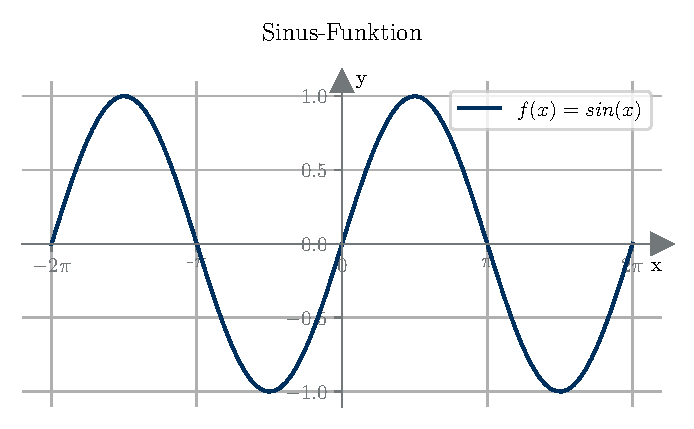
\includegraphics[clip, width=0.8\textwidth]{sinus}};
                %\helplines
            \end{tikzpicture}
        \end{center}
        \caption{Ein PDF-Plot aus \matplotlib.}\label{fig:pdf-plot}
    \end{figure}

    Die Einbindung erfolgt mit dem folgenden Code:

    \begin{minipage}{\textwidth}
\begin{lstlisting}[language=TeX,label={lst:include-pdf}, style=latexstyle, caption=Einbindung eines pdf-plots]
\begin{figure}[htb]
    \begin{center}
        \begin{tikzpicture}
            \node[inner sep=0pt, outer sep=0pt] (test) at (0,0) {
                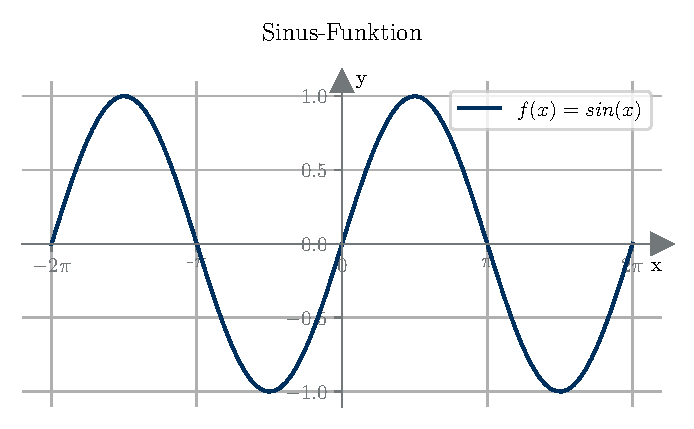
\includegraphics[clip, width=0.8\textwidth]{sinus}};
            %\helplines
        \end{tikzpicture}
    \end{center}
    \caption{Ein PDF-Plot aus \matplotlib.}\label{fig:pdf-plot}
\end{figure}
\end{lstlisting}
    \end{minipage}

    \subsection{Vergleich}\label{subsec:vergleich}

    Der Vergleich der beiden Plots ist noch einmal in \autoref{fig:pdf-pgf-comparison} dargestellt.
    Es zeigt sich, dass z.\@\,B.\@ bei der Änderung der Textbreite -- von den ursprünglich für die Berechnung der Grafiken verwendeten 418.25555 Punkten auf 455.24417 Punkte -- durch die Verwendung des Schalters \lstinline[language=Tex, style=latexstyle]|cd=true| der Dokumentenklasse tudscrartcl ein Unterschied entsteht.
    In der PDF-Variante wird der Text nicht passend skaliert und wirkt dadurch in diesem Fall größer.

    \begin{figure}[htb]
        \begin{minipage}[b]{0.45\textwidth}
            \centering
            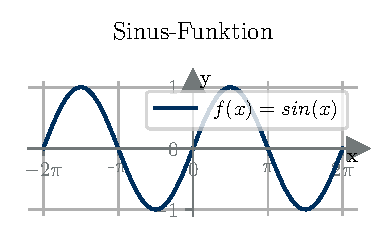
\includegraphics[width=\textwidth]{sinus_045}
        \end{minipage}
        \hfill
        \begin{minipage}[b]{0.45\textwidth}
            \centering
            %% Creator: Matplotlib, PGF backend
%%
%% To include the figure in your LaTeX document, write
%%   \input{<filename>.pgf}
%%
%% Make sure the required packages are loaded in your preamble
%%   \usepackage{pgf}
%%
%% Also ensure that all the required font packages are loaded; for instance,
%% the lmodern package is sometimes necessary when using math font.
%%   \usepackage{lmodern}
%%
%% Figures using additional raster images can only be included by \input if
%% they are in the same directory as the main LaTeX file. For loading figures
%% from other directories you can use the `import` package
%%   \usepackage{import}
%%
%% and then include the figures with
%%   \import{<path to file>}{<filename>.pgf}
%%
%% Matplotlib used the following preamble
%%   \def\mathdefault#1{#1}
%%   \everymath=\expandafter{\the\everymath\displaystyle}
%%   
%%   \makeatletter\@ifpackageloaded{underscore}{}{\usepackage[strings]{underscore}}\makeatother
%%
\begingroup%
\makeatletter%
\begin{pgfpicture}%
\pgfpathrectangle{\pgfpointorigin}{\pgfqpoint{2.604331in}{1.609565in}}%
\pgfusepath{use as bounding box, clip}%
\begin{pgfscope}%
\pgfsetbuttcap%
\pgfsetmiterjoin%
\definecolor{currentfill}{rgb}{1.000000,1.000000,1.000000}%
\pgfsetfillcolor{currentfill}%
\pgfsetlinewidth{0.000000pt}%
\definecolor{currentstroke}{rgb}{1.000000,1.000000,1.000000}%
\pgfsetstrokecolor{currentstroke}%
\pgfsetdash{}{0pt}%
\pgfpathmoveto{\pgfqpoint{0.000000in}{0.000000in}}%
\pgfpathlineto{\pgfqpoint{2.604331in}{0.000000in}}%
\pgfpathlineto{\pgfqpoint{2.604331in}{1.609565in}}%
\pgfpathlineto{\pgfqpoint{0.000000in}{1.609565in}}%
\pgfpathlineto{\pgfqpoint{0.000000in}{0.000000in}}%
\pgfpathclose%
\pgfusepath{fill}%
\end{pgfscope}%
\begin{pgfscope}%
\pgfsetbuttcap%
\pgfsetmiterjoin%
\definecolor{currentfill}{rgb}{1.000000,1.000000,1.000000}%
\pgfsetfillcolor{currentfill}%
\pgfsetlinewidth{0.000000pt}%
\definecolor{currentstroke}{rgb}{0.000000,0.000000,0.000000}%
\pgfsetstrokecolor{currentstroke}%
\pgfsetstrokeopacity{0.000000}%
\pgfsetdash{}{0pt}%
\pgfpathmoveto{\pgfqpoint{0.189068in}{0.168968in}}%
\pgfpathlineto{\pgfqpoint{2.384887in}{0.168968in}}%
\pgfpathlineto{\pgfqpoint{2.384887in}{1.066047in}}%
\pgfpathlineto{\pgfqpoint{0.189068in}{1.066047in}}%
\pgfpathlineto{\pgfqpoint{0.189068in}{0.168968in}}%
\pgfpathclose%
\pgfusepath{fill}%
\end{pgfscope}%
\begin{pgfscope}%
\pgfpathrectangle{\pgfqpoint{0.189068in}{0.168968in}}{\pgfqpoint{2.195818in}{0.897079in}}%
\pgfusepath{clip}%
\pgfsetrectcap%
\pgfsetroundjoin%
\pgfsetlinewidth{0.803000pt}%
\definecolor{currentstroke}{rgb}{0.690196,0.690196,0.690196}%
\pgfsetstrokecolor{currentstroke}%
\pgfsetdash{}{0pt}%
\pgfpathmoveto{\pgfqpoint{0.288878in}{0.168968in}}%
\pgfpathlineto{\pgfqpoint{0.288878in}{1.066047in}}%
\pgfusepath{stroke}%
\end{pgfscope}%
\begin{pgfscope}%
\pgfsetbuttcap%
\pgfsetroundjoin%
\definecolor{currentfill}{rgb}{0.447059,0.470588,0.474510}%
\pgfsetfillcolor{currentfill}%
\pgfsetlinewidth{0.803000pt}%
\definecolor{currentstroke}{rgb}{0.447059,0.470588,0.474510}%
\pgfsetstrokecolor{currentstroke}%
\pgfsetdash{}{0pt}%
\pgfsys@defobject{currentmarker}{\pgfqpoint{0.000000in}{-0.048611in}}{\pgfqpoint{0.000000in}{0.000000in}}{%
\pgfpathmoveto{\pgfqpoint{0.000000in}{0.000000in}}%
\pgfpathlineto{\pgfqpoint{0.000000in}{-0.048611in}}%
\pgfusepath{stroke,fill}%
}%
\begin{pgfscope}%
\pgfsys@transformshift{0.288878in}{0.617507in}%
\pgfsys@useobject{currentmarker}{}%
\end{pgfscope}%
\end{pgfscope}%
\begin{pgfscope}%
\definecolor{textcolor}{rgb}{0.447059,0.470588,0.474510}%
\pgfsetstrokecolor{textcolor}%
\pgfsetfillcolor{textcolor}%
\pgftext[x=0.288878in,y=0.520285in,,top]{\color{textcolor}{\rmfamily\fontsize{10.000000}{12.000000}\selectfont\catcode`\^=\active\def^{\ifmmode\sp\else\^{}\fi}\catcode`\%=\active\def%{\%}$-2\pi$}}%
\end{pgfscope}%
\begin{pgfscope}%
\pgfpathrectangle{\pgfqpoint{0.189068in}{0.168968in}}{\pgfqpoint{2.195818in}{0.897079in}}%
\pgfusepath{clip}%
\pgfsetrectcap%
\pgfsetroundjoin%
\pgfsetlinewidth{0.803000pt}%
\definecolor{currentstroke}{rgb}{0.690196,0.690196,0.690196}%
\pgfsetstrokecolor{currentstroke}%
\pgfsetdash{}{0pt}%
\pgfpathmoveto{\pgfqpoint{0.787928in}{0.168968in}}%
\pgfpathlineto{\pgfqpoint{0.787928in}{1.066047in}}%
\pgfusepath{stroke}%
\end{pgfscope}%
\begin{pgfscope}%
\pgfsetbuttcap%
\pgfsetroundjoin%
\definecolor{currentfill}{rgb}{0.447059,0.470588,0.474510}%
\pgfsetfillcolor{currentfill}%
\pgfsetlinewidth{0.803000pt}%
\definecolor{currentstroke}{rgb}{0.447059,0.470588,0.474510}%
\pgfsetstrokecolor{currentstroke}%
\pgfsetdash{}{0pt}%
\pgfsys@defobject{currentmarker}{\pgfqpoint{0.000000in}{-0.048611in}}{\pgfqpoint{0.000000in}{0.000000in}}{%
\pgfpathmoveto{\pgfqpoint{0.000000in}{0.000000in}}%
\pgfpathlineto{\pgfqpoint{0.000000in}{-0.048611in}}%
\pgfusepath{stroke,fill}%
}%
\begin{pgfscope}%
\pgfsys@transformshift{0.787928in}{0.617507in}%
\pgfsys@useobject{currentmarker}{}%
\end{pgfscope}%
\end{pgfscope}%
\begin{pgfscope}%
\definecolor{textcolor}{rgb}{0.447059,0.470588,0.474510}%
\pgfsetstrokecolor{textcolor}%
\pgfsetfillcolor{textcolor}%
\pgftext[x=0.787928in,y=0.520285in,,top]{\color{textcolor}{\rmfamily\fontsize{10.000000}{12.000000}\selectfont\catcode`\^=\active\def^{\ifmmode\sp\else\^{}\fi}\catcode`\%=\active\def%{\%}-$\pi$}}%
\end{pgfscope}%
\begin{pgfscope}%
\pgfpathrectangle{\pgfqpoint{0.189068in}{0.168968in}}{\pgfqpoint{2.195818in}{0.897079in}}%
\pgfusepath{clip}%
\pgfsetrectcap%
\pgfsetroundjoin%
\pgfsetlinewidth{0.803000pt}%
\definecolor{currentstroke}{rgb}{0.690196,0.690196,0.690196}%
\pgfsetstrokecolor{currentstroke}%
\pgfsetdash{}{0pt}%
\pgfpathmoveto{\pgfqpoint{1.286977in}{0.168968in}}%
\pgfpathlineto{\pgfqpoint{1.286977in}{1.066047in}}%
\pgfusepath{stroke}%
\end{pgfscope}%
\begin{pgfscope}%
\pgfsetbuttcap%
\pgfsetroundjoin%
\definecolor{currentfill}{rgb}{0.447059,0.470588,0.474510}%
\pgfsetfillcolor{currentfill}%
\pgfsetlinewidth{0.803000pt}%
\definecolor{currentstroke}{rgb}{0.447059,0.470588,0.474510}%
\pgfsetstrokecolor{currentstroke}%
\pgfsetdash{}{0pt}%
\pgfsys@defobject{currentmarker}{\pgfqpoint{0.000000in}{-0.048611in}}{\pgfqpoint{0.000000in}{0.000000in}}{%
\pgfpathmoveto{\pgfqpoint{0.000000in}{0.000000in}}%
\pgfpathlineto{\pgfqpoint{0.000000in}{-0.048611in}}%
\pgfusepath{stroke,fill}%
}%
\begin{pgfscope}%
\pgfsys@transformshift{1.286977in}{0.617507in}%
\pgfsys@useobject{currentmarker}{}%
\end{pgfscope}%
\end{pgfscope}%
\begin{pgfscope}%
\definecolor{textcolor}{rgb}{0.447059,0.470588,0.474510}%
\pgfsetstrokecolor{textcolor}%
\pgfsetfillcolor{textcolor}%
\pgftext[x=1.286977in,y=0.520285in,,top]{\color{textcolor}{\rmfamily\fontsize{10.000000}{12.000000}\selectfont\catcode`\^=\active\def^{\ifmmode\sp\else\^{}\fi}\catcode`\%=\active\def%{\%}0}}%
\end{pgfscope}%
\begin{pgfscope}%
\pgfpathrectangle{\pgfqpoint{0.189068in}{0.168968in}}{\pgfqpoint{2.195818in}{0.897079in}}%
\pgfusepath{clip}%
\pgfsetrectcap%
\pgfsetroundjoin%
\pgfsetlinewidth{0.803000pt}%
\definecolor{currentstroke}{rgb}{0.690196,0.690196,0.690196}%
\pgfsetstrokecolor{currentstroke}%
\pgfsetdash{}{0pt}%
\pgfpathmoveto{\pgfqpoint{1.786027in}{0.168968in}}%
\pgfpathlineto{\pgfqpoint{1.786027in}{1.066047in}}%
\pgfusepath{stroke}%
\end{pgfscope}%
\begin{pgfscope}%
\pgfsetbuttcap%
\pgfsetroundjoin%
\definecolor{currentfill}{rgb}{0.447059,0.470588,0.474510}%
\pgfsetfillcolor{currentfill}%
\pgfsetlinewidth{0.803000pt}%
\definecolor{currentstroke}{rgb}{0.447059,0.470588,0.474510}%
\pgfsetstrokecolor{currentstroke}%
\pgfsetdash{}{0pt}%
\pgfsys@defobject{currentmarker}{\pgfqpoint{0.000000in}{-0.048611in}}{\pgfqpoint{0.000000in}{0.000000in}}{%
\pgfpathmoveto{\pgfqpoint{0.000000in}{0.000000in}}%
\pgfpathlineto{\pgfqpoint{0.000000in}{-0.048611in}}%
\pgfusepath{stroke,fill}%
}%
\begin{pgfscope}%
\pgfsys@transformshift{1.786027in}{0.617507in}%
\pgfsys@useobject{currentmarker}{}%
\end{pgfscope}%
\end{pgfscope}%
\begin{pgfscope}%
\definecolor{textcolor}{rgb}{0.447059,0.470588,0.474510}%
\pgfsetstrokecolor{textcolor}%
\pgfsetfillcolor{textcolor}%
\pgftext[x=1.786027in,y=0.520285in,,top]{\color{textcolor}{\rmfamily\fontsize{10.000000}{12.000000}\selectfont\catcode`\^=\active\def^{\ifmmode\sp\else\^{}\fi}\catcode`\%=\active\def%{\%}$\pi$}}%
\end{pgfscope}%
\begin{pgfscope}%
\pgfpathrectangle{\pgfqpoint{0.189068in}{0.168968in}}{\pgfqpoint{2.195818in}{0.897079in}}%
\pgfusepath{clip}%
\pgfsetrectcap%
\pgfsetroundjoin%
\pgfsetlinewidth{0.803000pt}%
\definecolor{currentstroke}{rgb}{0.690196,0.690196,0.690196}%
\pgfsetstrokecolor{currentstroke}%
\pgfsetdash{}{0pt}%
\pgfpathmoveto{\pgfqpoint{2.285077in}{0.168968in}}%
\pgfpathlineto{\pgfqpoint{2.285077in}{1.066047in}}%
\pgfusepath{stroke}%
\end{pgfscope}%
\begin{pgfscope}%
\pgfsetbuttcap%
\pgfsetroundjoin%
\definecolor{currentfill}{rgb}{0.447059,0.470588,0.474510}%
\pgfsetfillcolor{currentfill}%
\pgfsetlinewidth{0.803000pt}%
\definecolor{currentstroke}{rgb}{0.447059,0.470588,0.474510}%
\pgfsetstrokecolor{currentstroke}%
\pgfsetdash{}{0pt}%
\pgfsys@defobject{currentmarker}{\pgfqpoint{0.000000in}{-0.048611in}}{\pgfqpoint{0.000000in}{0.000000in}}{%
\pgfpathmoveto{\pgfqpoint{0.000000in}{0.000000in}}%
\pgfpathlineto{\pgfqpoint{0.000000in}{-0.048611in}}%
\pgfusepath{stroke,fill}%
}%
\begin{pgfscope}%
\pgfsys@transformshift{2.285077in}{0.617507in}%
\pgfsys@useobject{currentmarker}{}%
\end{pgfscope}%
\end{pgfscope}%
\begin{pgfscope}%
\definecolor{textcolor}{rgb}{0.447059,0.470588,0.474510}%
\pgfsetstrokecolor{textcolor}%
\pgfsetfillcolor{textcolor}%
\pgftext[x=2.285077in,y=0.520285in,,top]{\color{textcolor}{\rmfamily\fontsize{10.000000}{12.000000}\selectfont\catcode`\^=\active\def^{\ifmmode\sp\else\^{}\fi}\catcode`\%=\active\def%{\%}$2\pi$}}%
\end{pgfscope}%
\begin{pgfscope}%
\pgfpathrectangle{\pgfqpoint{0.189068in}{0.168968in}}{\pgfqpoint{2.195818in}{0.897079in}}%
\pgfusepath{clip}%
\pgfsetrectcap%
\pgfsetroundjoin%
\pgfsetlinewidth{0.803000pt}%
\definecolor{currentstroke}{rgb}{0.690196,0.690196,0.690196}%
\pgfsetstrokecolor{currentstroke}%
\pgfsetdash{}{0pt}%
\pgfpathmoveto{\pgfqpoint{0.189068in}{0.209693in}}%
\pgfpathlineto{\pgfqpoint{2.384887in}{0.209693in}}%
\pgfusepath{stroke}%
\end{pgfscope}%
\begin{pgfscope}%
\pgfsetbuttcap%
\pgfsetroundjoin%
\definecolor{currentfill}{rgb}{0.447059,0.470588,0.474510}%
\pgfsetfillcolor{currentfill}%
\pgfsetlinewidth{0.803000pt}%
\definecolor{currentstroke}{rgb}{0.447059,0.470588,0.474510}%
\pgfsetstrokecolor{currentstroke}%
\pgfsetdash{}{0pt}%
\pgfsys@defobject{currentmarker}{\pgfqpoint{-0.048611in}{0.000000in}}{\pgfqpoint{-0.000000in}{0.000000in}}{%
\pgfpathmoveto{\pgfqpoint{-0.000000in}{0.000000in}}%
\pgfpathlineto{\pgfqpoint{-0.048611in}{0.000000in}}%
\pgfusepath{stroke,fill}%
}%
\begin{pgfscope}%
\pgfsys@transformshift{1.286977in}{0.209693in}%
\pgfsys@useobject{currentmarker}{}%
\end{pgfscope}%
\end{pgfscope}%
\begin{pgfscope}%
\definecolor{textcolor}{rgb}{0.447059,0.470588,0.474510}%
\pgfsetstrokecolor{textcolor}%
\pgfsetfillcolor{textcolor}%
\pgftext[x=1.012285in, y=0.161467in, left, base]{\color{textcolor}{\rmfamily\fontsize{10.000000}{12.000000}\selectfont\catcode`\^=\active\def^{\ifmmode\sp\else\^{}\fi}\catcode`\%=\active\def%{\%}$\mathdefault{\ensuremath{-}1}$}}%
\end{pgfscope}%
\begin{pgfscope}%
\pgfpathrectangle{\pgfqpoint{0.189068in}{0.168968in}}{\pgfqpoint{2.195818in}{0.897079in}}%
\pgfusepath{clip}%
\pgfsetrectcap%
\pgfsetroundjoin%
\pgfsetlinewidth{0.803000pt}%
\definecolor{currentstroke}{rgb}{0.690196,0.690196,0.690196}%
\pgfsetstrokecolor{currentstroke}%
\pgfsetdash{}{0pt}%
\pgfpathmoveto{\pgfqpoint{0.189068in}{0.617507in}}%
\pgfpathlineto{\pgfqpoint{2.384887in}{0.617507in}}%
\pgfusepath{stroke}%
\end{pgfscope}%
\begin{pgfscope}%
\pgfsetbuttcap%
\pgfsetroundjoin%
\definecolor{currentfill}{rgb}{0.447059,0.470588,0.474510}%
\pgfsetfillcolor{currentfill}%
\pgfsetlinewidth{0.803000pt}%
\definecolor{currentstroke}{rgb}{0.447059,0.470588,0.474510}%
\pgfsetstrokecolor{currentstroke}%
\pgfsetdash{}{0pt}%
\pgfsys@defobject{currentmarker}{\pgfqpoint{-0.048611in}{0.000000in}}{\pgfqpoint{-0.000000in}{0.000000in}}{%
\pgfpathmoveto{\pgfqpoint{-0.000000in}{0.000000in}}%
\pgfpathlineto{\pgfqpoint{-0.048611in}{0.000000in}}%
\pgfusepath{stroke,fill}%
}%
\begin{pgfscope}%
\pgfsys@transformshift{1.286977in}{0.617507in}%
\pgfsys@useobject{currentmarker}{}%
\end{pgfscope}%
\end{pgfscope}%
\begin{pgfscope}%
\definecolor{textcolor}{rgb}{0.447059,0.470588,0.474510}%
\pgfsetstrokecolor{textcolor}%
\pgfsetfillcolor{textcolor}%
\pgftext[x=1.120310in, y=0.569282in, left, base]{\color{textcolor}{\rmfamily\fontsize{10.000000}{12.000000}\selectfont\catcode`\^=\active\def^{\ifmmode\sp\else\^{}\fi}\catcode`\%=\active\def%{\%}$\mathdefault{0}$}}%
\end{pgfscope}%
\begin{pgfscope}%
\pgfpathrectangle{\pgfqpoint{0.189068in}{0.168968in}}{\pgfqpoint{2.195818in}{0.897079in}}%
\pgfusepath{clip}%
\pgfsetrectcap%
\pgfsetroundjoin%
\pgfsetlinewidth{0.803000pt}%
\definecolor{currentstroke}{rgb}{0.690196,0.690196,0.690196}%
\pgfsetstrokecolor{currentstroke}%
\pgfsetdash{}{0pt}%
\pgfpathmoveto{\pgfqpoint{0.189068in}{1.025322in}}%
\pgfpathlineto{\pgfqpoint{2.384887in}{1.025322in}}%
\pgfusepath{stroke}%
\end{pgfscope}%
\begin{pgfscope}%
\pgfsetbuttcap%
\pgfsetroundjoin%
\definecolor{currentfill}{rgb}{0.447059,0.470588,0.474510}%
\pgfsetfillcolor{currentfill}%
\pgfsetlinewidth{0.803000pt}%
\definecolor{currentstroke}{rgb}{0.447059,0.470588,0.474510}%
\pgfsetstrokecolor{currentstroke}%
\pgfsetdash{}{0pt}%
\pgfsys@defobject{currentmarker}{\pgfqpoint{-0.048611in}{0.000000in}}{\pgfqpoint{-0.000000in}{0.000000in}}{%
\pgfpathmoveto{\pgfqpoint{-0.000000in}{0.000000in}}%
\pgfpathlineto{\pgfqpoint{-0.048611in}{0.000000in}}%
\pgfusepath{stroke,fill}%
}%
\begin{pgfscope}%
\pgfsys@transformshift{1.286977in}{1.025322in}%
\pgfsys@useobject{currentmarker}{}%
\end{pgfscope}%
\end{pgfscope}%
\begin{pgfscope}%
\definecolor{textcolor}{rgb}{0.447059,0.470588,0.474510}%
\pgfsetstrokecolor{textcolor}%
\pgfsetfillcolor{textcolor}%
\pgftext[x=1.120310in, y=0.977097in, left, base]{\color{textcolor}{\rmfamily\fontsize{10.000000}{12.000000}\selectfont\catcode`\^=\active\def^{\ifmmode\sp\else\^{}\fi}\catcode`\%=\active\def%{\%}$\mathdefault{1}$}}%
\end{pgfscope}%
\begin{pgfscope}%
\pgfpathrectangle{\pgfqpoint{0.189068in}{0.168968in}}{\pgfqpoint{2.195818in}{0.897079in}}%
\pgfusepath{clip}%
\pgfsetrectcap%
\pgfsetroundjoin%
\pgfsetlinewidth{1.505625pt}%
\definecolor{currentstroke}{rgb}{0.000000,0.188235,0.368627}%
\pgfsetstrokecolor{currentstroke}%
\pgfsetdash{}{0pt}%
\pgfpathmoveto{\pgfqpoint{0.288878in}{0.617507in}}%
\pgfpathlineto{\pgfqpoint{0.309042in}{0.669133in}}%
\pgfpathlineto{\pgfqpoint{0.329205in}{0.719929in}}%
\pgfpathlineto{\pgfqpoint{0.349369in}{0.769077in}}%
\pgfpathlineto{\pgfqpoint{0.369533in}{0.815785in}}%
\pgfpathlineto{\pgfqpoint{0.389696in}{0.859304in}}%
\pgfpathlineto{\pgfqpoint{0.409860in}{0.898932in}}%
\pgfpathlineto{\pgfqpoint{0.430023in}{0.934031in}}%
\pgfpathlineto{\pgfqpoint{0.450187in}{0.964038in}}%
\pgfpathlineto{\pgfqpoint{0.470351in}{0.988468in}}%
\pgfpathlineto{\pgfqpoint{0.490514in}{1.006930in}}%
\pgfpathlineto{\pgfqpoint{0.510678in}{1.019126in}}%
\pgfpathlineto{\pgfqpoint{0.530842in}{1.024860in}}%
\pgfpathlineto{\pgfqpoint{0.551005in}{1.024039in}}%
\pgfpathlineto{\pgfqpoint{0.571169in}{1.016677in}}%
\pgfpathlineto{\pgfqpoint{0.591332in}{1.002892in}}%
\pgfpathlineto{\pgfqpoint{0.611496in}{0.982907in}}%
\pgfpathlineto{\pgfqpoint{0.631660in}{0.957041in}}%
\pgfpathlineto{\pgfqpoint{0.651823in}{0.925713in}}%
\pgfpathlineto{\pgfqpoint{0.671987in}{0.889425in}}%
\pgfpathlineto{\pgfqpoint{0.692150in}{0.848763in}}%
\pgfpathlineto{\pgfqpoint{0.712314in}{0.804379in}}%
\pgfpathlineto{\pgfqpoint{0.732478in}{0.756988in}}%
\pgfpathlineto{\pgfqpoint{0.752641in}{0.707353in}}%
\pgfpathlineto{\pgfqpoint{0.772805in}{0.656272in}}%
\pgfpathlineto{\pgfqpoint{0.792969in}{0.604568in}}%
\pgfpathlineto{\pgfqpoint{0.813132in}{0.553072in}}%
\pgfpathlineto{\pgfqpoint{0.833296in}{0.502613in}}%
\pgfpathlineto{\pgfqpoint{0.853459in}{0.454002in}}%
\pgfpathlineto{\pgfqpoint{0.873623in}{0.408022in}}%
\pgfpathlineto{\pgfqpoint{0.893787in}{0.365413in}}%
\pgfpathlineto{\pgfqpoint{0.913950in}{0.326860in}}%
\pgfpathlineto{\pgfqpoint{0.934114in}{0.292984in}}%
\pgfpathlineto{\pgfqpoint{0.954278in}{0.264329in}}%
\pgfpathlineto{\pgfqpoint{0.974441in}{0.241358in}}%
\pgfpathlineto{\pgfqpoint{0.994605in}{0.224438in}}%
\pgfpathlineto{\pgfqpoint{1.014768in}{0.213843in}}%
\pgfpathlineto{\pgfqpoint{1.034932in}{0.209744in}}%
\pgfpathlineto{\pgfqpoint{1.055096in}{0.212205in}}%
\pgfpathlineto{\pgfqpoint{1.075259in}{0.221188in}}%
\pgfpathlineto{\pgfqpoint{1.095423in}{0.236548in}}%
\pgfpathlineto{\pgfqpoint{1.115587in}{0.258038in}}%
\pgfpathlineto{\pgfqpoint{1.135750in}{0.285311in}}%
\pgfpathlineto{\pgfqpoint{1.155914in}{0.317930in}}%
\pgfpathlineto{\pgfqpoint{1.176077in}{0.355369in}}%
\pgfpathlineto{\pgfqpoint{1.196241in}{0.397026in}}%
\pgfpathlineto{\pgfqpoint{1.216405in}{0.442231in}}%
\pgfpathlineto{\pgfqpoint{1.236568in}{0.490255in}}%
\pgfpathlineto{\pgfqpoint{1.256732in}{0.540328in}}%
\pgfpathlineto{\pgfqpoint{1.276896in}{0.591642in}}%
\pgfpathlineto{\pgfqpoint{1.297059in}{0.643372in}}%
\pgfpathlineto{\pgfqpoint{1.317223in}{0.694687in}}%
\pgfpathlineto{\pgfqpoint{1.337386in}{0.744759in}}%
\pgfpathlineto{\pgfqpoint{1.357550in}{0.792784in}}%
\pgfpathlineto{\pgfqpoint{1.377714in}{0.837988in}}%
\pgfpathlineto{\pgfqpoint{1.397877in}{0.879645in}}%
\pgfpathlineto{\pgfqpoint{1.418041in}{0.917084in}}%
\pgfpathlineto{\pgfqpoint{1.438204in}{0.949703in}}%
\pgfpathlineto{\pgfqpoint{1.458368in}{0.976977in}}%
\pgfpathlineto{\pgfqpoint{1.478532in}{0.998466in}}%
\pgfpathlineto{\pgfqpoint{1.498695in}{1.013826in}}%
\pgfpathlineto{\pgfqpoint{1.518859in}{1.022809in}}%
\pgfpathlineto{\pgfqpoint{1.539023in}{1.025271in}}%
\pgfpathlineto{\pgfqpoint{1.559186in}{1.021171in}}%
\pgfpathlineto{\pgfqpoint{1.579350in}{1.010576in}}%
\pgfpathlineto{\pgfqpoint{1.599513in}{0.993657in}}%
\pgfpathlineto{\pgfqpoint{1.619677in}{0.970685in}}%
\pgfpathlineto{\pgfqpoint{1.639841in}{0.942031in}}%
\pgfpathlineto{\pgfqpoint{1.660004in}{0.908154in}}%
\pgfpathlineto{\pgfqpoint{1.680168in}{0.869601in}}%
\pgfpathlineto{\pgfqpoint{1.700332in}{0.826992in}}%
\pgfpathlineto{\pgfqpoint{1.720495in}{0.781013in}}%
\pgfpathlineto{\pgfqpoint{1.740659in}{0.732402in}}%
\pgfpathlineto{\pgfqpoint{1.760822in}{0.681942in}}%
\pgfpathlineto{\pgfqpoint{1.780986in}{0.630446in}}%
\pgfpathlineto{\pgfqpoint{1.801150in}{0.578742in}}%
\pgfpathlineto{\pgfqpoint{1.821313in}{0.527661in}}%
\pgfpathlineto{\pgfqpoint{1.841477in}{0.478026in}}%
\pgfpathlineto{\pgfqpoint{1.861641in}{0.430636in}}%
\pgfpathlineto{\pgfqpoint{1.881804in}{0.386252in}}%
\pgfpathlineto{\pgfqpoint{1.901968in}{0.345589in}}%
\pgfpathlineto{\pgfqpoint{1.922131in}{0.309301in}}%
\pgfpathlineto{\pgfqpoint{1.942295in}{0.277973in}}%
\pgfpathlineto{\pgfqpoint{1.962459in}{0.252108in}}%
\pgfpathlineto{\pgfqpoint{1.982622in}{0.232122in}}%
\pgfpathlineto{\pgfqpoint{2.002786in}{0.218337in}}%
\pgfpathlineto{\pgfqpoint{2.022949in}{0.210975in}}%
\pgfpathlineto{\pgfqpoint{2.043113in}{0.210154in}}%
\pgfpathlineto{\pgfqpoint{2.063277in}{0.215888in}}%
\pgfpathlineto{\pgfqpoint{2.083440in}{0.228084in}}%
\pgfpathlineto{\pgfqpoint{2.103604in}{0.246546in}}%
\pgfpathlineto{\pgfqpoint{2.123768in}{0.270977in}}%
\pgfpathlineto{\pgfqpoint{2.143931in}{0.300983in}}%
\pgfpathlineto{\pgfqpoint{2.164095in}{0.336083in}}%
\pgfpathlineto{\pgfqpoint{2.184258in}{0.375711in}}%
\pgfpathlineto{\pgfqpoint{2.204422in}{0.419229in}}%
\pgfpathlineto{\pgfqpoint{2.224586in}{0.465938in}}%
\pgfpathlineto{\pgfqpoint{2.244749in}{0.515085in}}%
\pgfpathlineto{\pgfqpoint{2.264913in}{0.565881in}}%
\pgfpathlineto{\pgfqpoint{2.285077in}{0.617507in}}%
\pgfusepath{stroke}%
\end{pgfscope}%
\begin{pgfscope}%
\pgfsetbuttcap%
\pgfsetmiterjoin%
\definecolor{currentfill}{rgb}{0.447059,0.470588,0.474510}%
\pgfsetfillcolor{currentfill}%
\pgfsetlinewidth{1.003750pt}%
\definecolor{currentstroke}{rgb}{0.447059,0.470588,0.474510}%
\pgfsetstrokecolor{currentstroke}%
\pgfsetdash{}{0pt}%
\pgfsys@defobject{currentmarker}{\pgfqpoint{-0.069444in}{-0.069444in}}{\pgfqpoint{0.069444in}{0.069444in}}{%
\pgfpathmoveto{\pgfqpoint{0.069444in}{-0.000000in}}%
\pgfpathlineto{\pgfqpoint{-0.069444in}{0.069444in}}%
\pgfpathlineto{\pgfqpoint{-0.069444in}{-0.069444in}}%
\pgfpathlineto{\pgfqpoint{0.069444in}{-0.000000in}}%
\pgfpathclose%
\pgfusepath{stroke,fill}%
}%
\begin{pgfscope}%
\pgfsys@transformshift{2.384887in}{0.617507in}%
\pgfsys@useobject{currentmarker}{}%
\end{pgfscope}%
\end{pgfscope}%
\begin{pgfscope}%
\pgfsetbuttcap%
\pgfsetmiterjoin%
\definecolor{currentfill}{rgb}{0.447059,0.470588,0.474510}%
\pgfsetfillcolor{currentfill}%
\pgfsetlinewidth{1.003750pt}%
\definecolor{currentstroke}{rgb}{0.447059,0.470588,0.474510}%
\pgfsetstrokecolor{currentstroke}%
\pgfsetdash{}{0pt}%
\pgfsys@defobject{currentmarker}{\pgfqpoint{-0.069444in}{-0.069444in}}{\pgfqpoint{0.069444in}{0.069444in}}{%
\pgfpathmoveto{\pgfqpoint{0.000000in}{0.069444in}}%
\pgfpathlineto{\pgfqpoint{-0.069444in}{-0.069444in}}%
\pgfpathlineto{\pgfqpoint{0.069444in}{-0.069444in}}%
\pgfpathlineto{\pgfqpoint{0.000000in}{0.069444in}}%
\pgfpathclose%
\pgfusepath{stroke,fill}%
}%
\begin{pgfscope}%
\pgfsys@transformshift{1.286977in}{1.066047in}%
\pgfsys@useobject{currentmarker}{}%
\end{pgfscope}%
\end{pgfscope}%
\begin{pgfscope}%
\pgfsetrectcap%
\pgfsetmiterjoin%
\pgfsetlinewidth{0.803000pt}%
\definecolor{currentstroke}{rgb}{0.447059,0.470588,0.474510}%
\pgfsetstrokecolor{currentstroke}%
\pgfsetdash{}{0pt}%
\pgfpathmoveto{\pgfqpoint{1.286977in}{0.168968in}}%
\pgfpathlineto{\pgfqpoint{1.286977in}{1.066047in}}%
\pgfusepath{stroke}%
\end{pgfscope}%
\begin{pgfscope}%
\pgfsetrectcap%
\pgfsetmiterjoin%
\pgfsetlinewidth{0.000000pt}%
\definecolor{currentstroke}{rgb}{0.000000,0.000000,0.000000}%
\pgfsetstrokecolor{currentstroke}%
\pgfsetstrokeopacity{0.000000}%
\pgfsetdash{}{0pt}%
\pgfpathmoveto{\pgfqpoint{2.384887in}{0.168968in}}%
\pgfpathlineto{\pgfqpoint{2.384887in}{1.066047in}}%
\pgfusepath{}%
\end{pgfscope}%
\begin{pgfscope}%
\pgfsetrectcap%
\pgfsetmiterjoin%
\pgfsetlinewidth{0.803000pt}%
\definecolor{currentstroke}{rgb}{0.447059,0.470588,0.474510}%
\pgfsetstrokecolor{currentstroke}%
\pgfsetdash{}{0pt}%
\pgfpathmoveto{\pgfqpoint{0.189068in}{0.617507in}}%
\pgfpathlineto{\pgfqpoint{2.384887in}{0.617507in}}%
\pgfusepath{stroke}%
\end{pgfscope}%
\begin{pgfscope}%
\pgfsetrectcap%
\pgfsetmiterjoin%
\pgfsetlinewidth{0.000000pt}%
\definecolor{currentstroke}{rgb}{0.000000,0.000000,0.000000}%
\pgfsetstrokecolor{currentstroke}%
\pgfsetstrokeopacity{0.000000}%
\pgfsetdash{}{0pt}%
\pgfpathmoveto{\pgfqpoint{0.189068in}{1.066047in}}%
\pgfpathlineto{\pgfqpoint{2.384887in}{1.066047in}}%
\pgfusepath{}%
\end{pgfscope}%
\begin{pgfscope}%
\definecolor{textcolor}{rgb}{0.000000,0.000000,0.000000}%
\pgfsetstrokecolor{textcolor}%
\pgfsetfillcolor{textcolor}%
\pgftext[x=2.384887in,y=0.556335in,right,]{\color{textcolor}{\rmfamily\fontsize{10.000000}{12.000000}\selectfont\catcode`\^=\active\def^{\ifmmode\sp\else\^{}\fi}\catcode`\%=\active\def%{\%}x}}%
\end{pgfscope}%
\begin{pgfscope}%
\definecolor{textcolor}{rgb}{0.000000,0.000000,0.000000}%
\pgfsetstrokecolor{textcolor}%
\pgfsetfillcolor{textcolor}%
\pgftext[x=1.334633in,y=1.066047in,left,]{\color{textcolor}{\rmfamily\fontsize{10.000000}{12.000000}\selectfont\catcode`\^=\active\def^{\ifmmode\sp\else\^{}\fi}\catcode`\%=\active\def%{\%}y}}%
\end{pgfscope}%
\begin{pgfscope}%
\definecolor{textcolor}{rgb}{0.000000,0.000000,0.000000}%
\pgfsetstrokecolor{textcolor}%
\pgfsetfillcolor{textcolor}%
\pgftext[x=1.286977in,y=1.343825in,,base]{\color{textcolor}{\rmfamily\fontsize{12.000000}{14.400000}\selectfont\catcode`\^=\active\def^{\ifmmode\sp\else\^{}\fi}\catcode`\%=\active\def%{\%}Sinus-Funktion}}%
\end{pgfscope}%
\begin{pgfscope}%
\pgfsetbuttcap%
\pgfsetmiterjoin%
\definecolor{currentfill}{rgb}{1.000000,1.000000,1.000000}%
\pgfsetfillcolor{currentfill}%
\pgfsetfillopacity{0.800000}%
\pgfsetlinewidth{1.003750pt}%
\definecolor{currentstroke}{rgb}{0.800000,0.800000,0.800000}%
\pgfsetstrokecolor{currentstroke}%
\pgfsetstrokeopacity{0.800000}%
\pgfsetdash{}{0pt}%
\pgfpathmoveto{\pgfqpoint{1.003962in}{0.746602in}}%
\pgfpathlineto{\pgfqpoint{2.287664in}{0.746602in}}%
\pgfpathquadraticcurveto{\pgfqpoint{2.315442in}{0.746602in}}{\pgfqpoint{2.315442in}{0.774380in}}%
\pgfpathlineto{\pgfqpoint{2.315442in}{0.968825in}}%
\pgfpathquadraticcurveto{\pgfqpoint{2.315442in}{0.996602in}}{\pgfqpoint{2.287664in}{0.996602in}}%
\pgfpathlineto{\pgfqpoint{1.003962in}{0.996602in}}%
\pgfpathquadraticcurveto{\pgfqpoint{0.976184in}{0.996602in}}{\pgfqpoint{0.976184in}{0.968825in}}%
\pgfpathlineto{\pgfqpoint{0.976184in}{0.774380in}}%
\pgfpathquadraticcurveto{\pgfqpoint{0.976184in}{0.746602in}}{\pgfqpoint{1.003962in}{0.746602in}}%
\pgfpathlineto{\pgfqpoint{1.003962in}{0.746602in}}%
\pgfpathclose%
\pgfusepath{stroke,fill}%
\end{pgfscope}%
\begin{pgfscope}%
\pgfsetrectcap%
\pgfsetroundjoin%
\pgfsetlinewidth{1.505625pt}%
\definecolor{currentstroke}{rgb}{0.000000,0.188235,0.368627}%
\pgfsetstrokecolor{currentstroke}%
\pgfsetdash{}{0pt}%
\pgfpathmoveto{\pgfqpoint{1.031739in}{0.885491in}}%
\pgfpathlineto{\pgfqpoint{1.170628in}{0.885491in}}%
\pgfpathlineto{\pgfqpoint{1.309517in}{0.885491in}}%
\pgfusepath{stroke}%
\end{pgfscope}%
\begin{pgfscope}%
\definecolor{textcolor}{rgb}{0.000000,0.000000,0.000000}%
\pgfsetstrokecolor{textcolor}%
\pgfsetfillcolor{textcolor}%
\pgftext[x=1.420628in,y=0.836880in,left,base]{\color{textcolor}{\rmfamily\fontsize{10.000000}{12.000000}\selectfont\catcode`\^=\active\def^{\ifmmode\sp\else\^{}\fi}\catcode`\%=\active\def%{\%}$f(x) = sin(x)$}}%
\end{pgfscope}%
\end{pgfpicture}%
\makeatother%
\endgroup%

        \end{minipage}
        \caption{Vergleich von PDF (links) und PGF (rechts).}\label{fig:pdf-pgf-comparison}
    \end{figure}




    %\typeout{cdgrey is: \csname\string\color@cdgrey\endcsname}
    %showthe{\cdgrey}

\end{document}